\documentclass[english,11pt]{beamer}

\DeclareMathOperator{\Cov}{Cov}
\DeclareMathOperator{\Var}{Var}
\DeclareMathOperator{\E}{\mathbb{E}}
\DeclareMathOperator{\Proba}{\mathbb{P}}

\newcommand{\Covb}[2]{\ensuremath{\Cov\!\left[#1,#2\right]}}
\newcommand{\Eb}[1]{\ensuremath{\E\!\left[#1\right]}}
\newcommand{\Pb}[1]{\ensuremath{\Proba\!\left[#1\right]}}
\newcommand{\Varb}[1]{\ensuremath{\Var\!\left[#1\right]}}

% norm
\newcommand{\norm}[1]{\| #1 \|}

\newcommand{\indep}{\rotatebox[origin=c]{90}{$\models$}}





\usepackage{mathptmx,amsmath,amssymb,graphicx,bibentry,bbm,babel,ragged2e}

\makeatletter

\newcommand{\noun}[1]{\textsc{#1}}
\newcommand{\jitem}[1]{\item \begin{justify} #1 \end{justify} \vfill{}}
\newcommand{\sframe}[2]{\frame{\frametitle{#1} #2}}

\newenvironment{centercolumns}{\begin{columns}[c]}{\end{columns}}
%\newenvironment{jitem}{\begin{justify}\begin{itemize}}{\end{itemize}\end{justify}}

\usetheme{Warsaw}
\setbeamertemplate{footline}[text line]{}
\setbeamercolor{structure}{fg=purple!50!blue, bg=purple!50!blue}

\setbeamersize{text margin left=15pt,text margin right=15pt}

\setbeamercovered{transparent}


\@ifundefined{showcaptionsetup}{}{%
 \PassOptionsToPackage{caption=false}{subfig}}
\usepackage{subfig}

\usepackage[utf8]{inputenc}
\usepackage[T1]{fontenc}

\usepackage{multirow}


\makeatother

\begin{document}





\title{Exploration et validation des modèles de simulation avec la plateforme ouverte OpenMOLE}

\author{J.~Raimbault$^{1,2,3,4,\ast}$\\
\texttt{$\ast$ juste.raimbault@ign.fr}
}


\institute{$^{1}$ LASTIG, IGN-ENSG\\
$^{2}$CASA, UCL\\
$^{3}$UPS CNRS 3611 ISC-PIF\\
$^{4}$UMR CNRS 8504 G{\'e}ographie-cit{\'e}s
}


\date{Journée d'étude Big Data et données spatialisées\\\smallskip
IGN\\\smallskip
29 Juin 2023
}

\frame{\maketitle}




\sframe{Modélisation et simulation en géographie}{

% Cette présentation propose d'illustrer la question de la validation des modèles de simulation, dans le cas particulier de la géographie

%The role of simulation models in the production of knowledge has significantly shifted in recent years, accompanied with a transformation of practices, including methods and tools. This presentation aims at describing these mutations from the point of view of theoretical and quantitative geography.

\begin{columns}

	\begin{column}{0.5\textwidth}
	\centering
	
	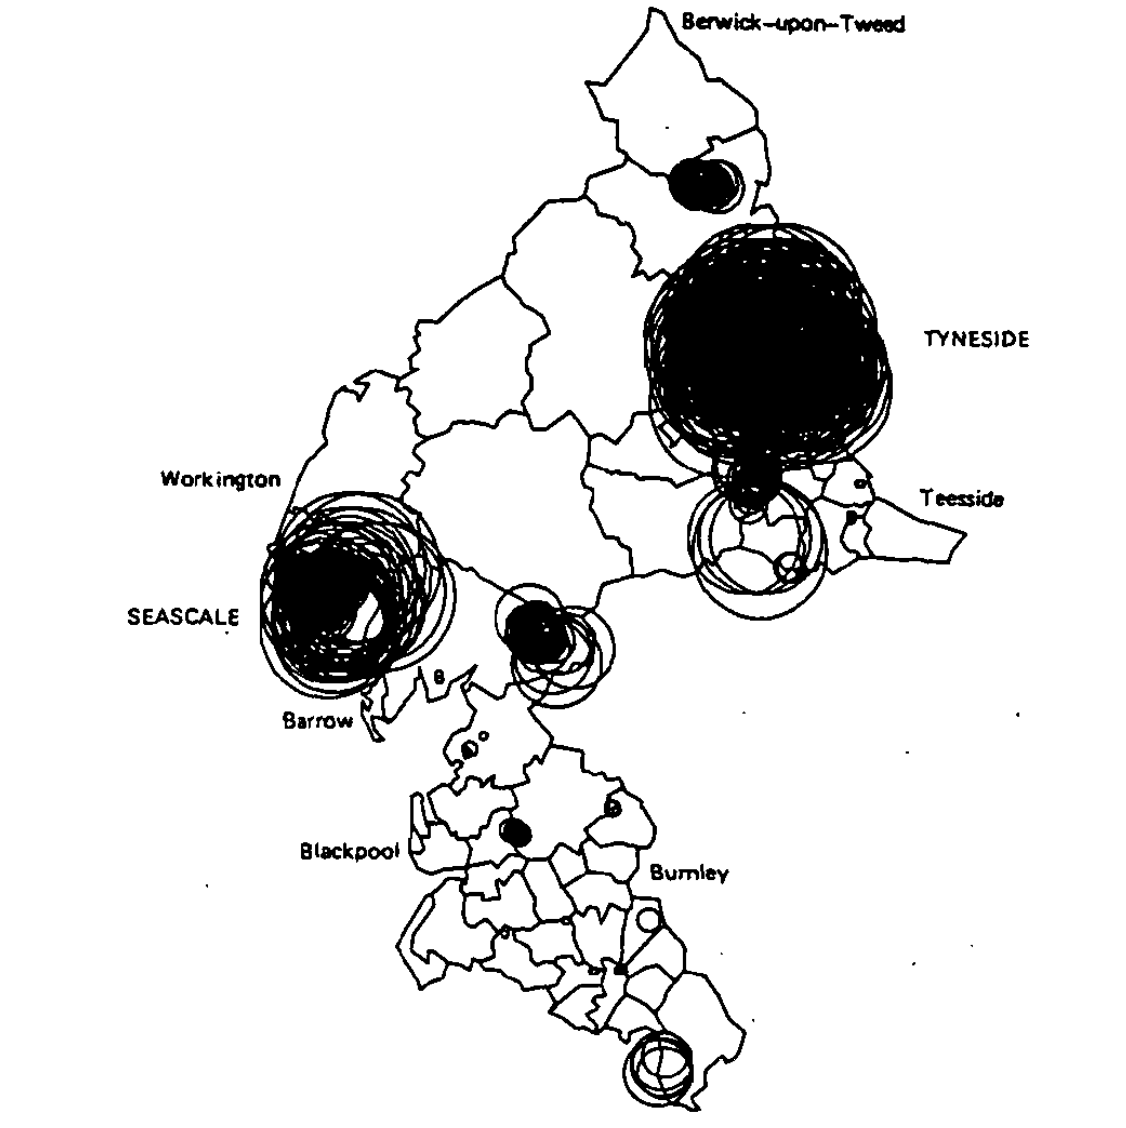
\includegraphics[width=0.6\textwidth]{figures/openshaw.png}
	
	\footnotesize
\textit{Machine d'analyse géographique \cite{openshaw1987mark}}
	
	\medskip
	\hrule
	\medskip
	
	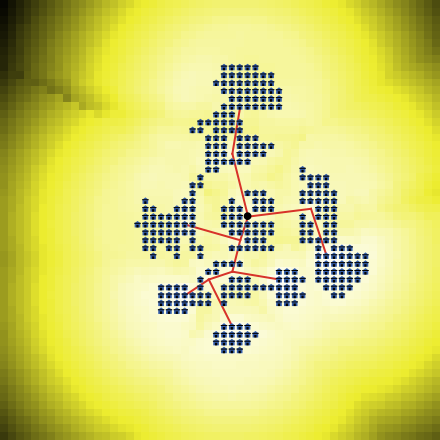
\includegraphics[width=0.55\textwidth,height=0.3\textheight]{figures/intro_RBD_lattice.png}
	
	\footnotesize
\textit{Morphogenèse urbaine hybride \cite{raimbault2014hybrid}}
	

	\end{column}
	\vrule{}
	\begin{column}{0.5\textwidth}
	\centering
	
	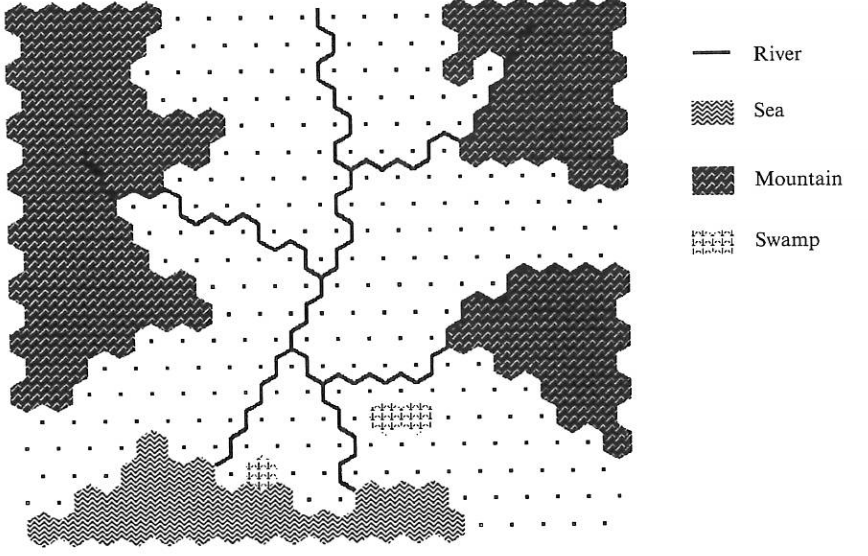
\includegraphics[width=0.7\textwidth]{figures/simpop1.png}
	
	\footnotesize
\textit{Modèle Simpop 1 \cite{sanders1997simpop}}

	\medskip

	\hrule
	
	\medskip

	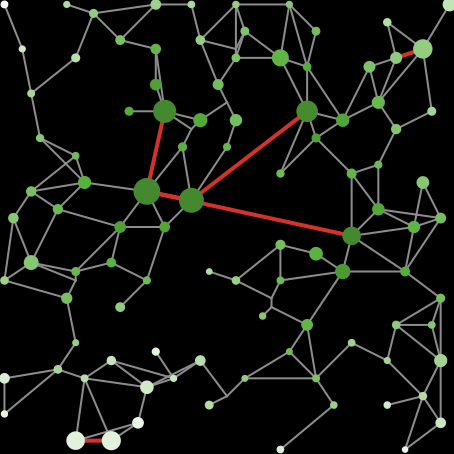
\includegraphics[width=0.6\textwidth]{figures/setup_synth_1_tick100.png}
	
	\footnotesize
	\textit{Modèle SimpopNet \cite{schmitt2014modelisation}}
	
	\end{column}


\end{columns}

}



\sframe{Systèmes géographique et complexité}{

% pour laquelle la prépondérance de l'espace augmente la complexité des modèles

\textit{Nécessité des modèles de simulation en géographie induite par les multiples complexités de ces systèmes ?}

\bigskip

\begin{itemize}
	\item Complexité ontologique \cite{pumain2003approche}
	\item Complexité dynamique: non-ergodicité et dépendance au chemin \cite{pumain2012urban}
	\item Complexité et co-évolution \cite{raimbault2021modeling}
	\item Complexité et emergence \cite{raimbault2020relating}
\end{itemize}

}


\sframe{Théories et modèles}{

% these seb ; bouquin Varenne
% at least two slides ; examples ?

% top down - deduction : christaller etc : theorie => empirique. validité logique et interne des principes initiaux.
% bottom up - induction : Hagget etc : empirique => theorique. validation empirique
% Pumain : epistemologie de synthese : quelles methodes de validation ?

Succession historique d'épistémologies dans le cas des systèmes de villes \cite{varenne2017theories}: 

\medskip

\begin{enumerate}
	\item Déduction depuis la théorie (top-down): Christaller
	\item Induction depuis l'empirique (bottom-up): Berry
	\item Vers une épistémologie abductive (interaction iterative théorique-empirique): Pumain
\end{enumerate}

\medskip

$\rightarrow$ la simulation permet la synthèse

}


\sframe{Validation des modèles de simulation}{

% Validation et verification : ingenierie systeme (external/internal) -> products what is expected and is close to reality
% philo : remplit ses fonctions ; laboratoire virtuel
% pratique : conceptual model validation / model verification
% manque d'outils

% vers une validation par l'evaluation ?

\justify

Multiples approches de la ``validation'' et ``verification'' des modèles 
\\\cite{rey2015plateforme}: origine dans l'ingénierie système; statut épistémologique lié aux fonctions du modèle; approches empiriques ad-hoc.

\medskip

\textit{Constat d'un manque d'outils}

\medskip

En pratique: tests unitaires du programme, validation interne, sorties visuelles, reproduction de motifs (quantitatif ou qualitatif), pouvoir prédictif, analyses de sensibilité.

$\rightarrow$ en pratique, peu de latitude sur les hypothèses théoriques et de modélisation; peu d'interaction entre les domaines de connaissance.

\medskip

\cite{rey2015plateforme}: vers une validation par l'évaluation (faits stylisés, pattern-oriented modeling, multi-modélisation) en interaction avec la théorie et l'empirique.


}



\sframe{Nouvelles méthodes pour la simulation en sciences sociales : ERC Geodivercity}{

% presentation generale de Geodivercity

\begin{columns}
\begin{column}{0.4\textwidth}
	\centering
	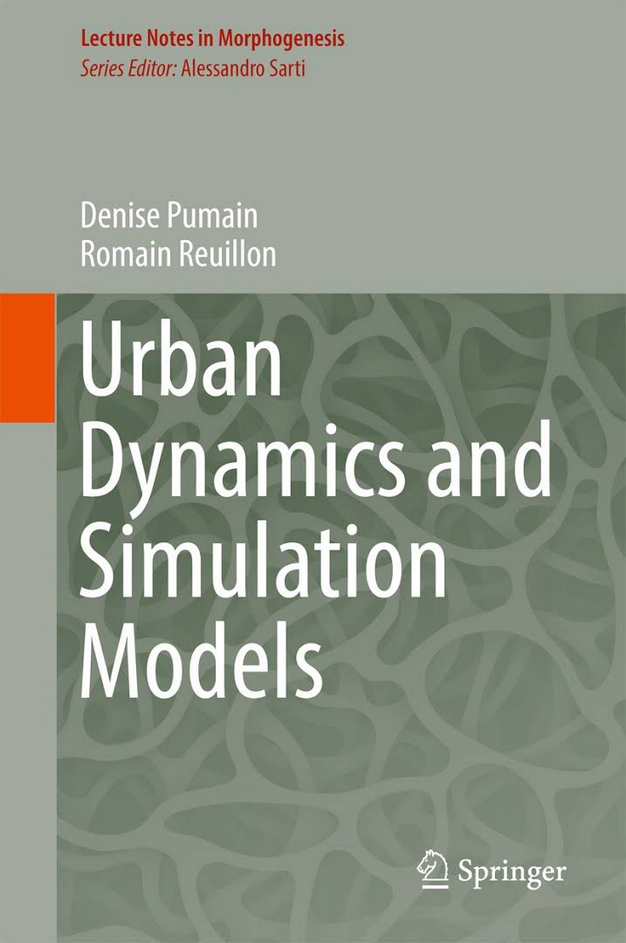
\includegraphics[width=\textwidth]{figures/urban-dynamics-simulation-models-geodivercity.png}
\end{column}
\begin{column}{0.6\textwidth}
	Développement de la théorie évolutive des villes \cite{pumain2018evolutionary}
	
	\medskip

	$\rightarrow$ Faits stylisés saillants pour l'ensemble des systèmes de villes principaux
	
	$\rightarrow$ Construction de modèles de simulation (modèles à visée explicative)
	
	$\rightarrow$ Outils et méthodes d'exploration des modèles de simulation : OpenMOLE développée principalement par R. Reuillon et M. Leclaire depuis 2008 à l'ISC-PIF
	
	\smallskip
	
	
	%
\includegraphics[width=\textwidth]{figures/openmole.png}
	% new logo!
	
\includegraphics[width=0.28\textwidth]{figures/iconOM.png}
	
\includegraphics[width=0.68\textwidth]{figures/openmole.png}
	
\end{column}
\end{columns}


}



\sframe{Environnement scientifique d'OpenMOLE \cite{raimbault2018extracting}}{

\centering

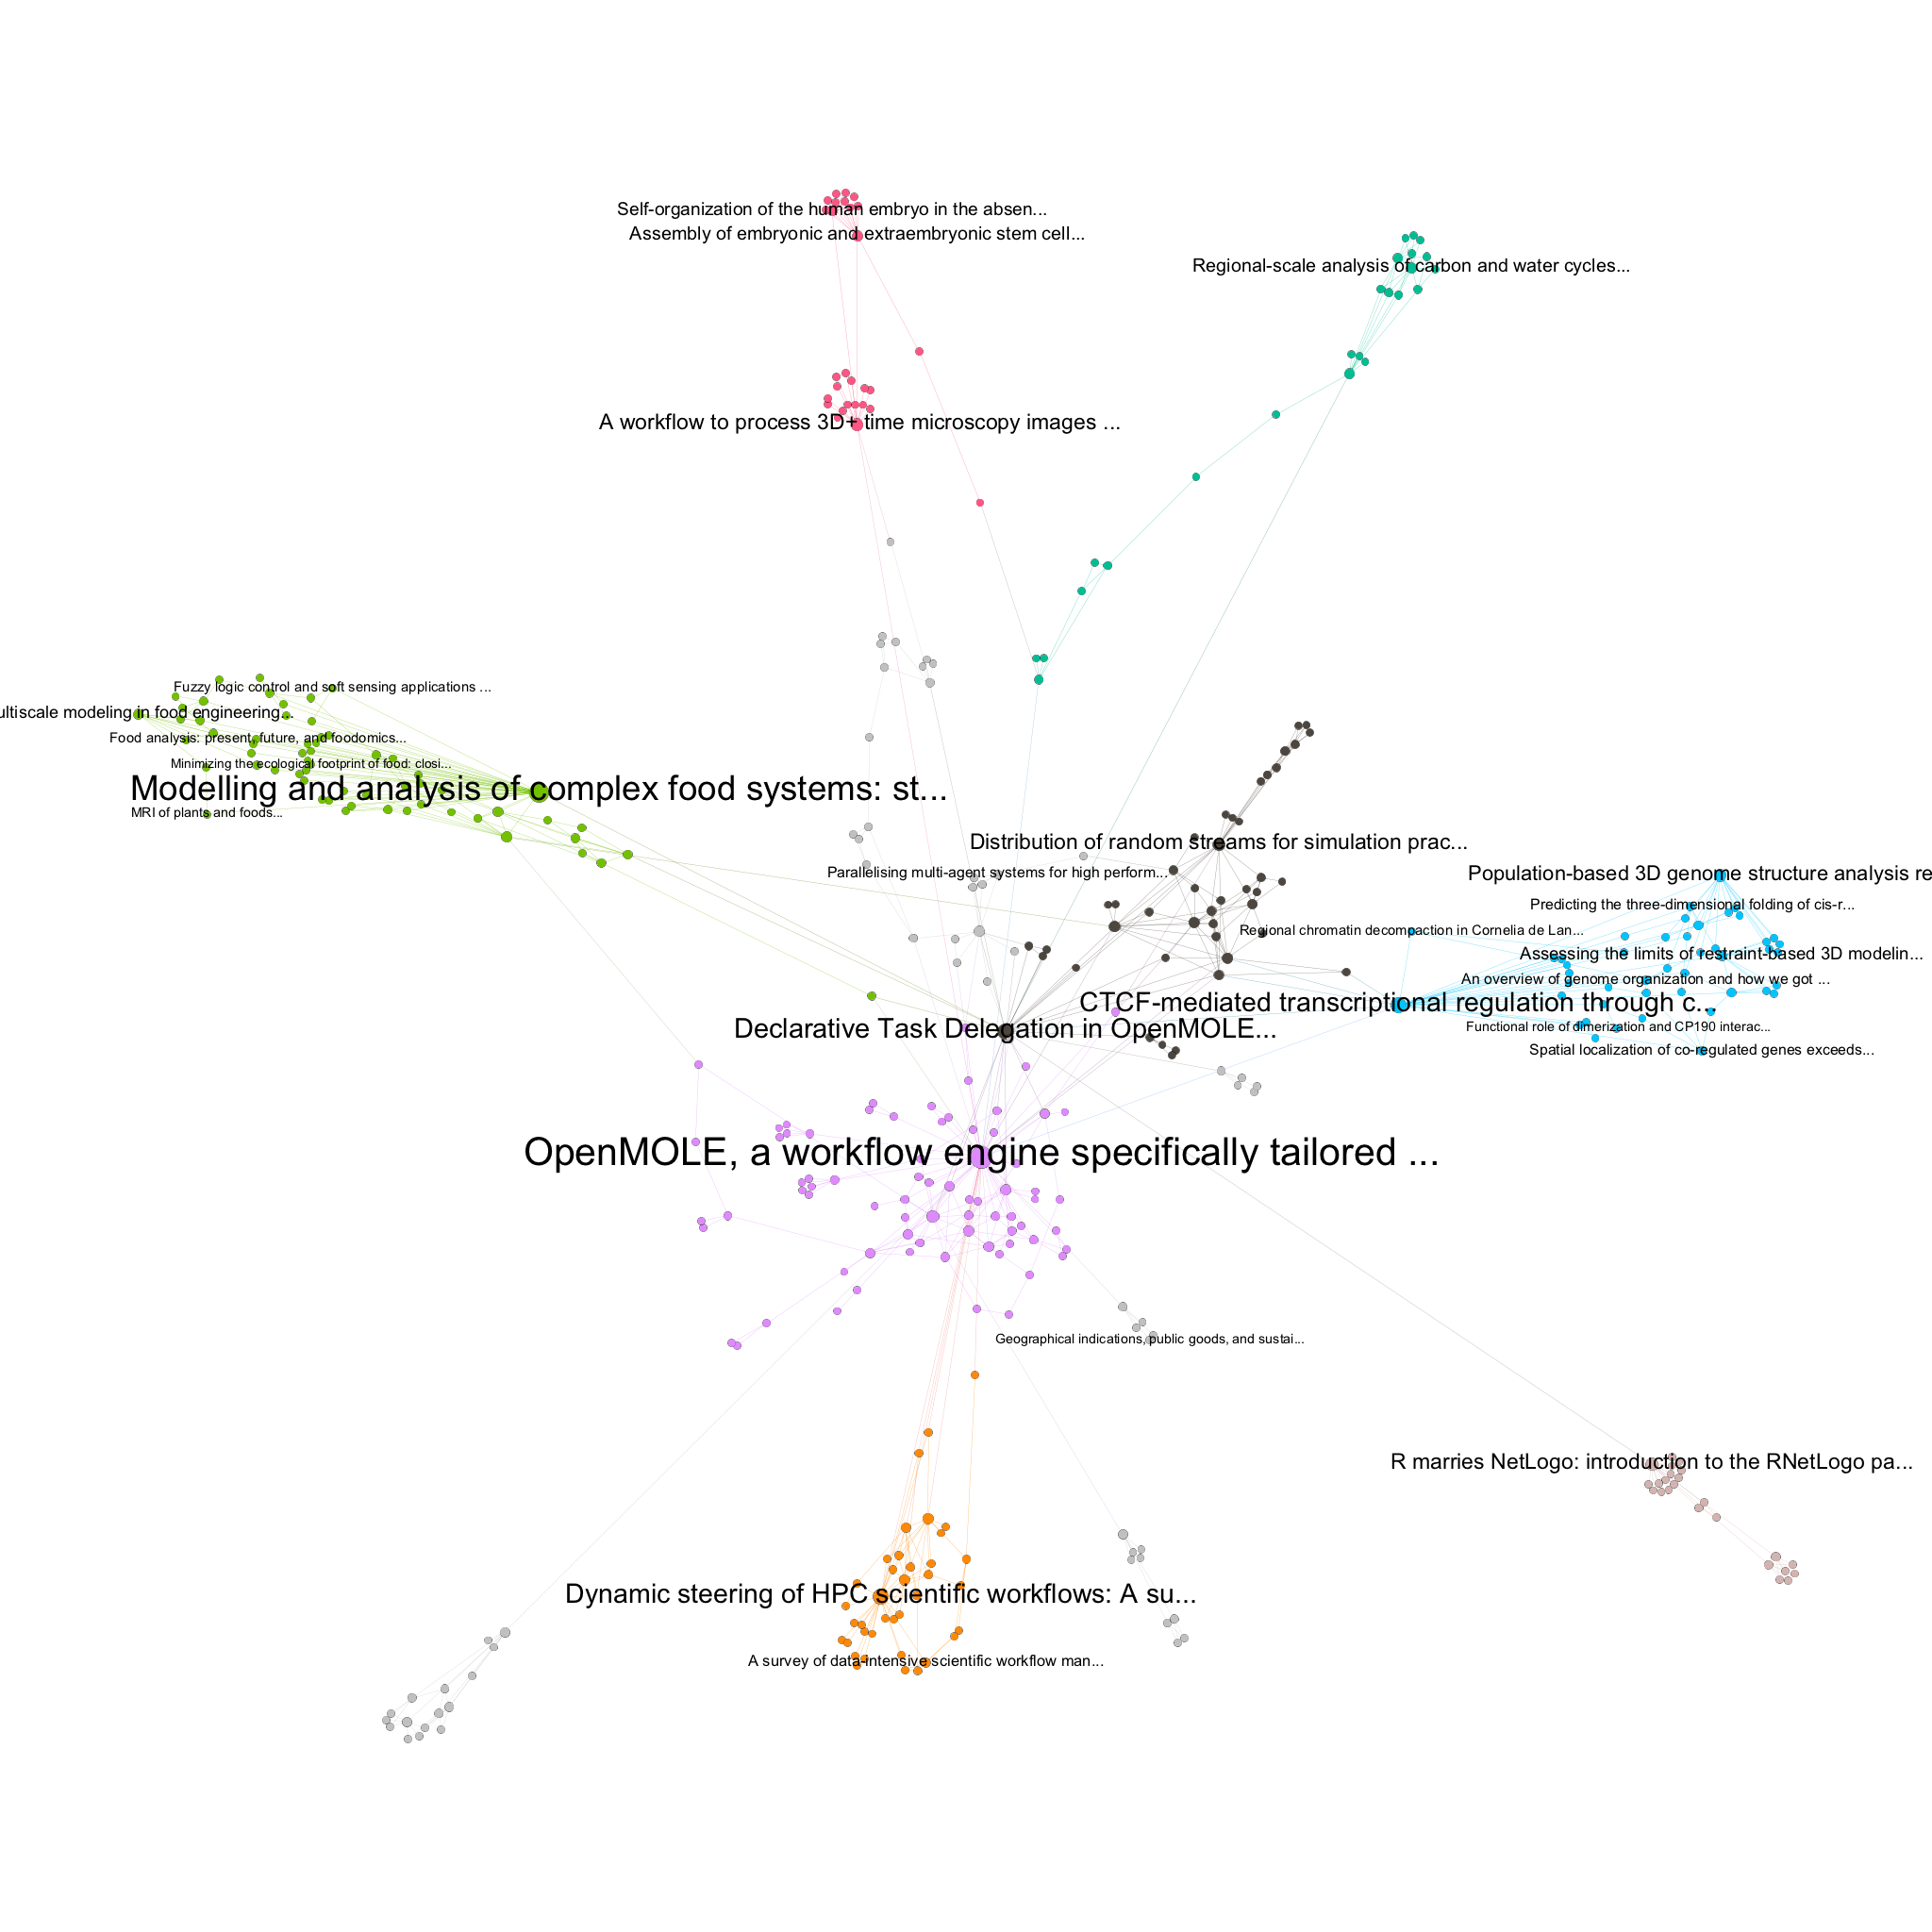
\includegraphics[width=\textwidth]{figures/oml_depth3_core.png}
}


%\sframe{Méthodes et outils: OpenMOLE}{
%}

\sframe{Principes d'OpenMOLE}{
	
	\footnotesize
	\textit{(i) Méthodes d'exploration et de validation innovantes; (ii) Passage à l'échelle par calcul distribué; (iii) Embarquement des modèles sans interférence.}
	
	\smallskip
	
	\centering
	
	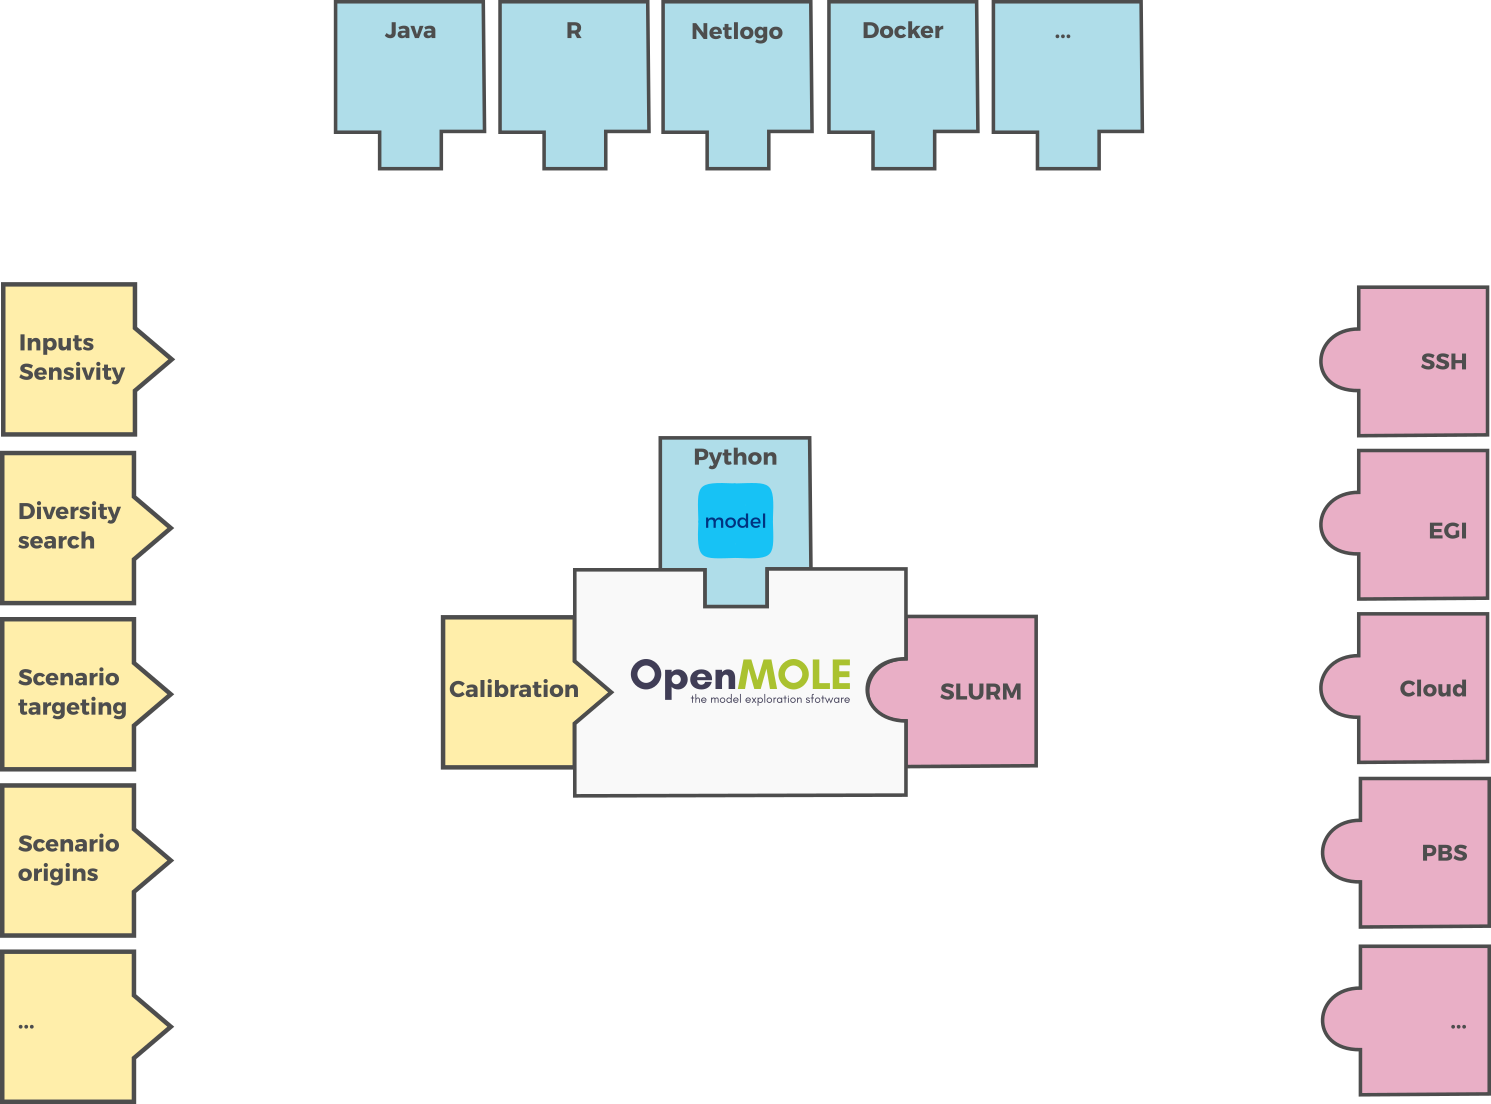
\includegraphics[width=0.9\textwidth]{figures/openmole_axis.png}
	
}





\sframe{Une interface web ergonomique}{

	\centering
	
	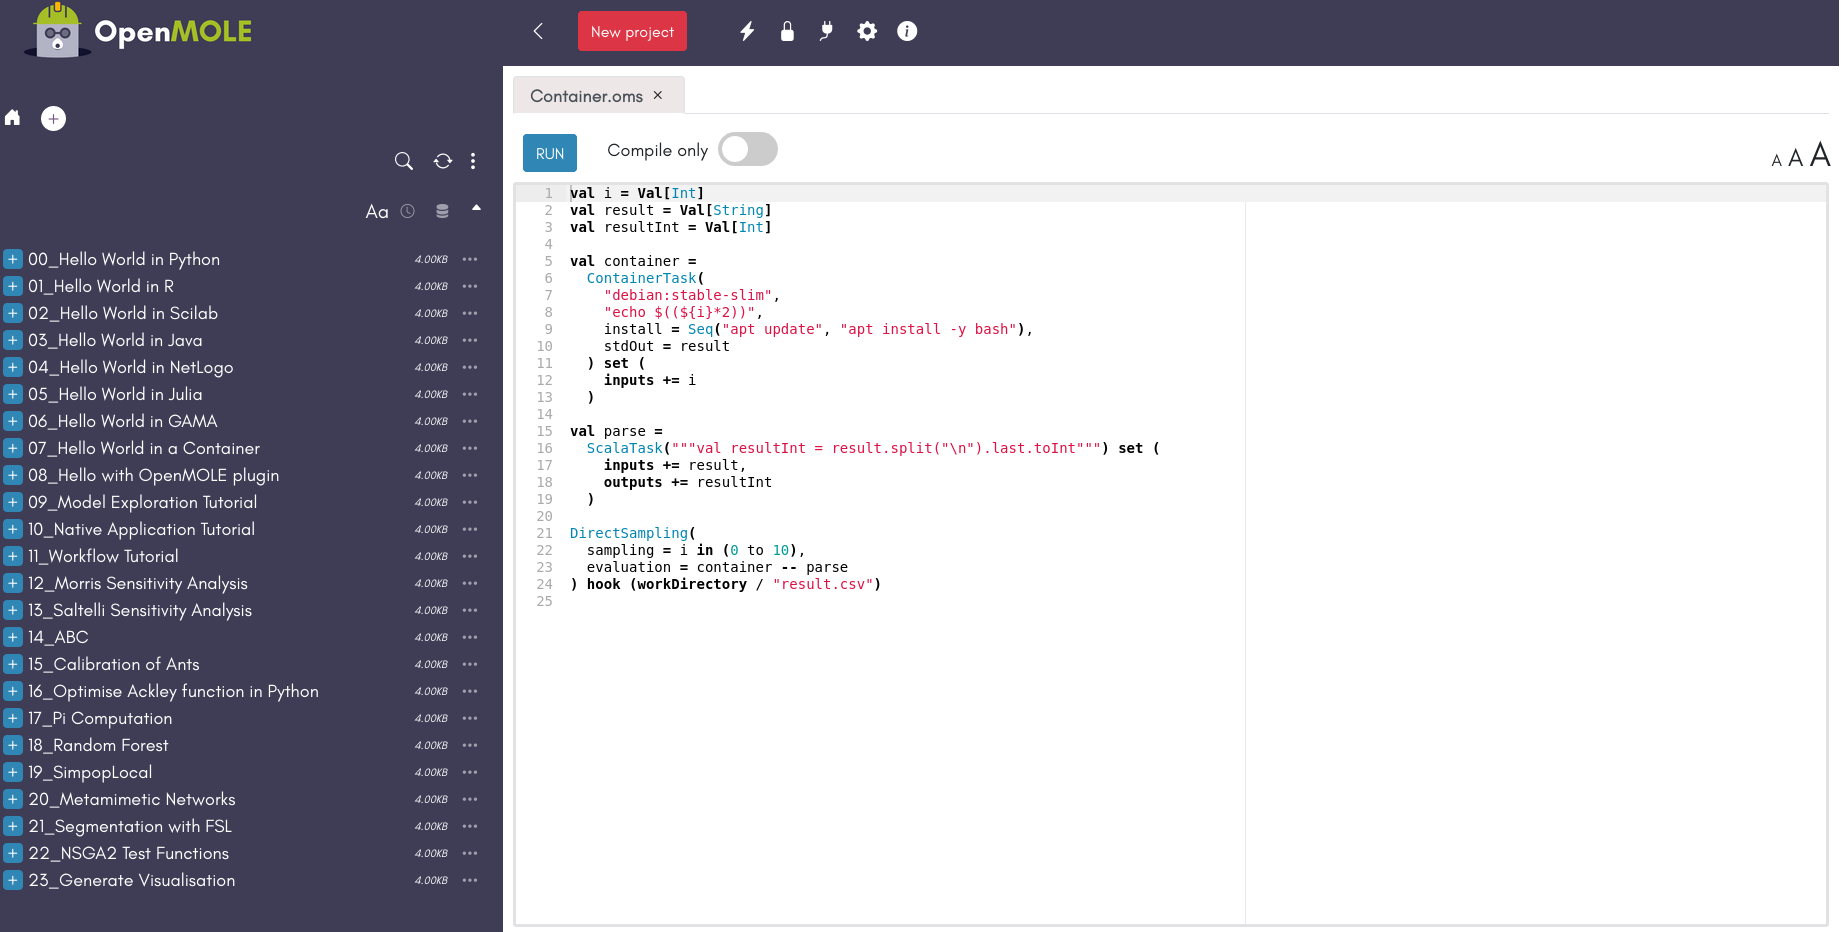
\includegraphics[width=\textwidth]{figures/openmolefirefox.png}
	
}

\sframe{Modèles de simulation}{

	\centering
	
	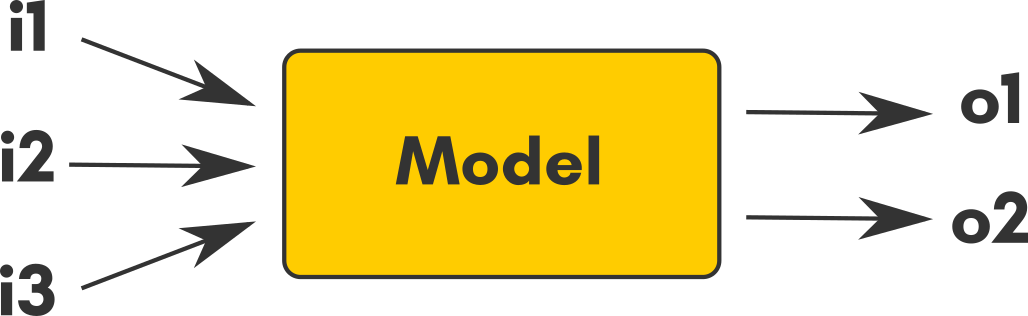
\includegraphics[width=\textwidth]{figures/modelIO.png}

}



\sframe{Agnostique aux langages}{

	\centering
	
	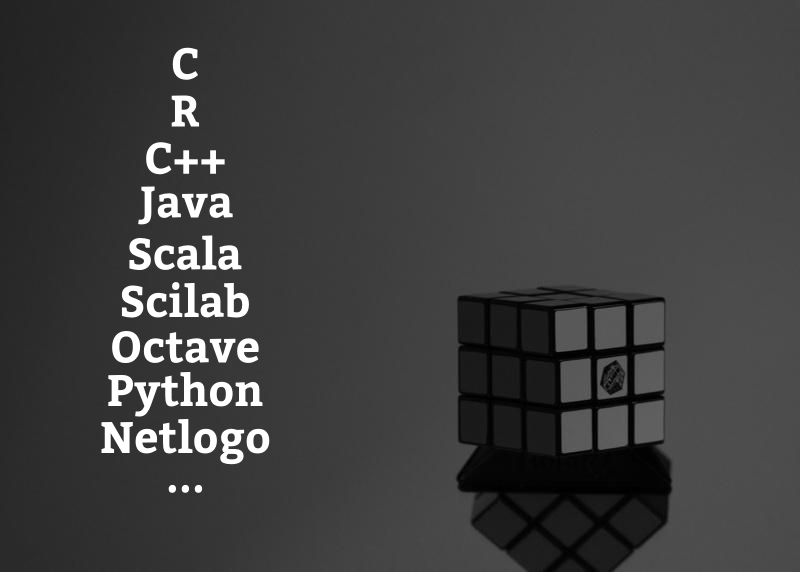
\includegraphics[width=\textwidth]{figures/blackbox.png}

}

\sframe{Modèle NetLogo}{

	
	\begin{center}
	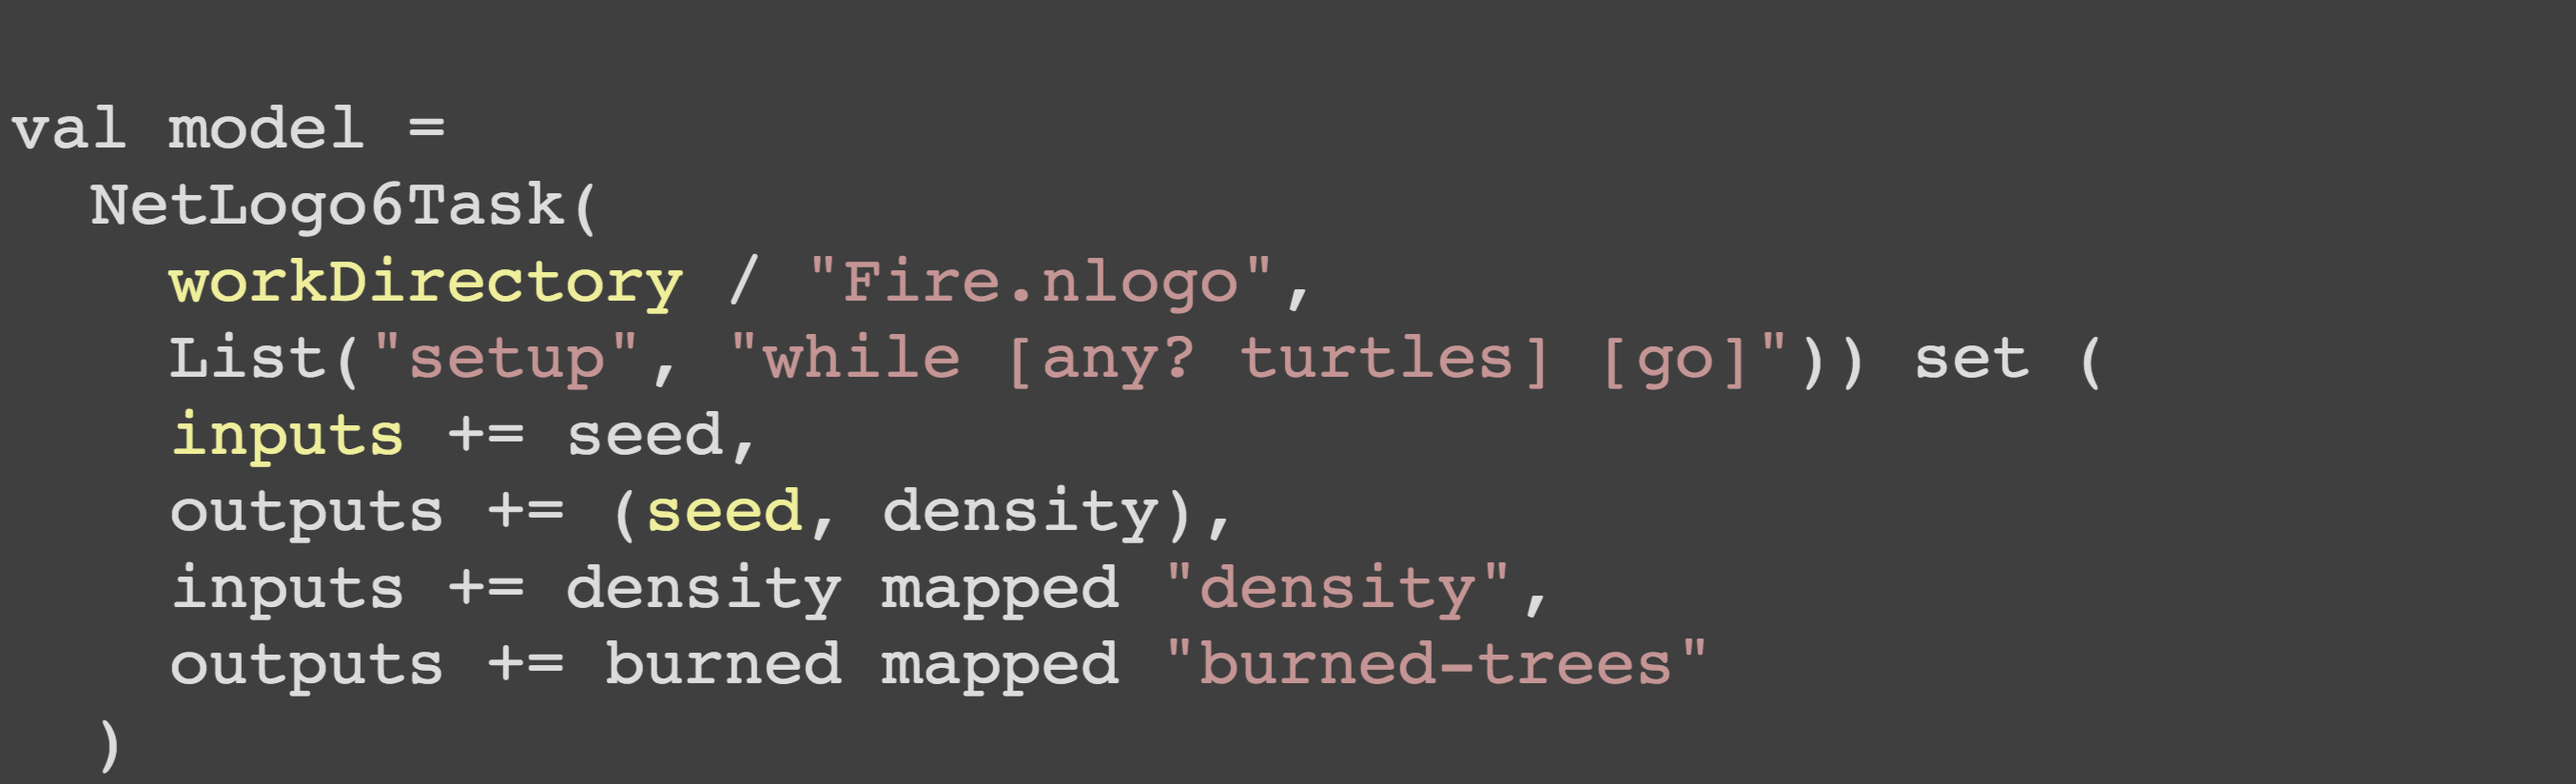
\includegraphics[width=\textwidth]{figures/netlogomodel.png}
	\end{center}	
	
	\bigskip
	
	DSL pour les scripts basé sur scala	
	
}

\sframe{Modèle R}{

	
	\begin{center}
	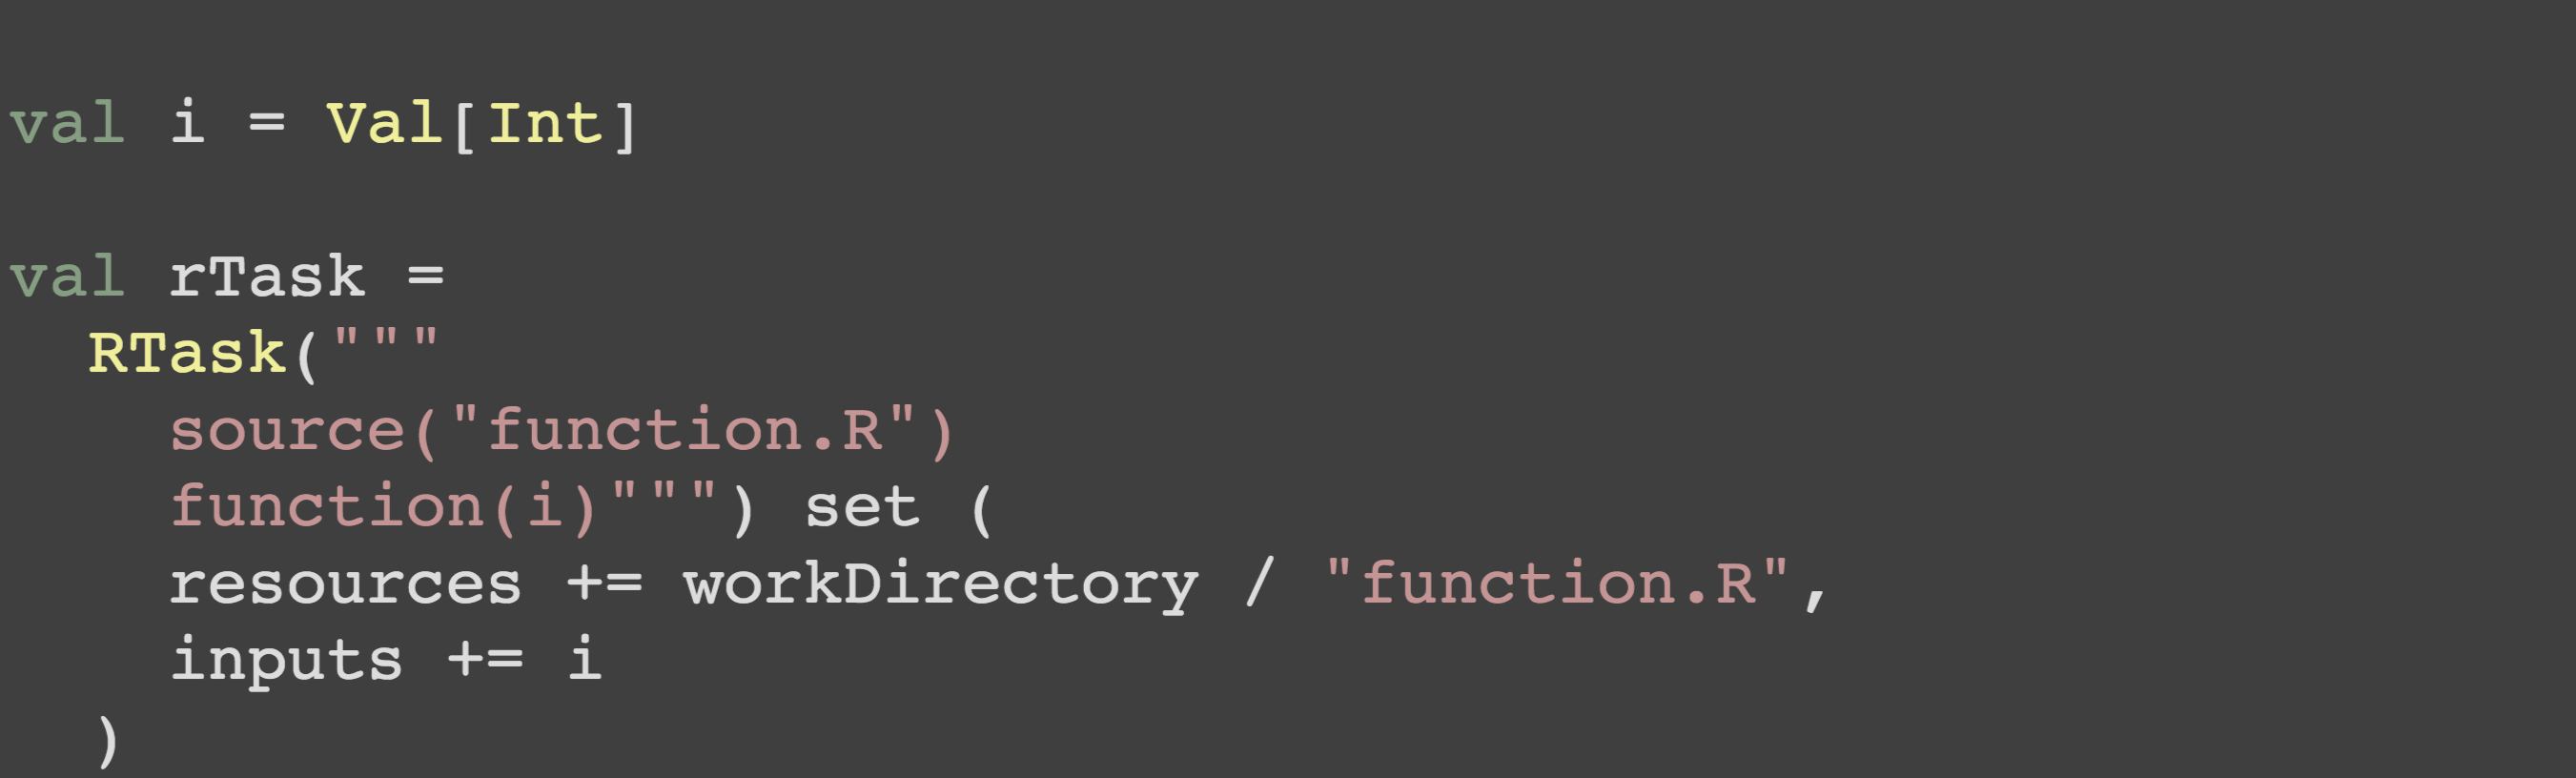
\includegraphics[width=\textwidth]{figures/rcode.png}
	\end{center}	
	
	\bigskip
	
	Syntaxe similaire pour la \texttt{PythonTask}
	
}

\sframe{Container docker}{


	\begin{center}
	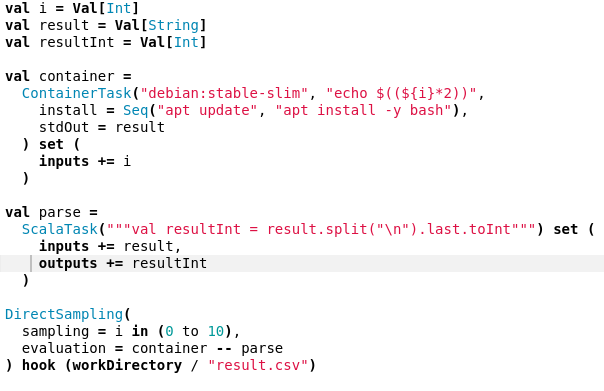
\includegraphics[width=\textwidth]{figures/container.png}
	\end{center}	
	

}



\sframe{Méthodes}{
	
	\begin{itemize}
		\item Estimation de paramètres
		\item Analyse de sensibilité
		\item Étude de robustesse
		\item Optimisation
	\end{itemize}

	% Designed in a scalable manner, handle stochasticity, usable on any models and environments
	
	\medskip
	
	\textit{Conçues pour passer à l'échelle, prendre en compte la stochasticité, être utilisable sur n'importe quel modèle et environnement de calcul.}
	
}

\sframe{Méthodes}{

	
	\begin{center}
	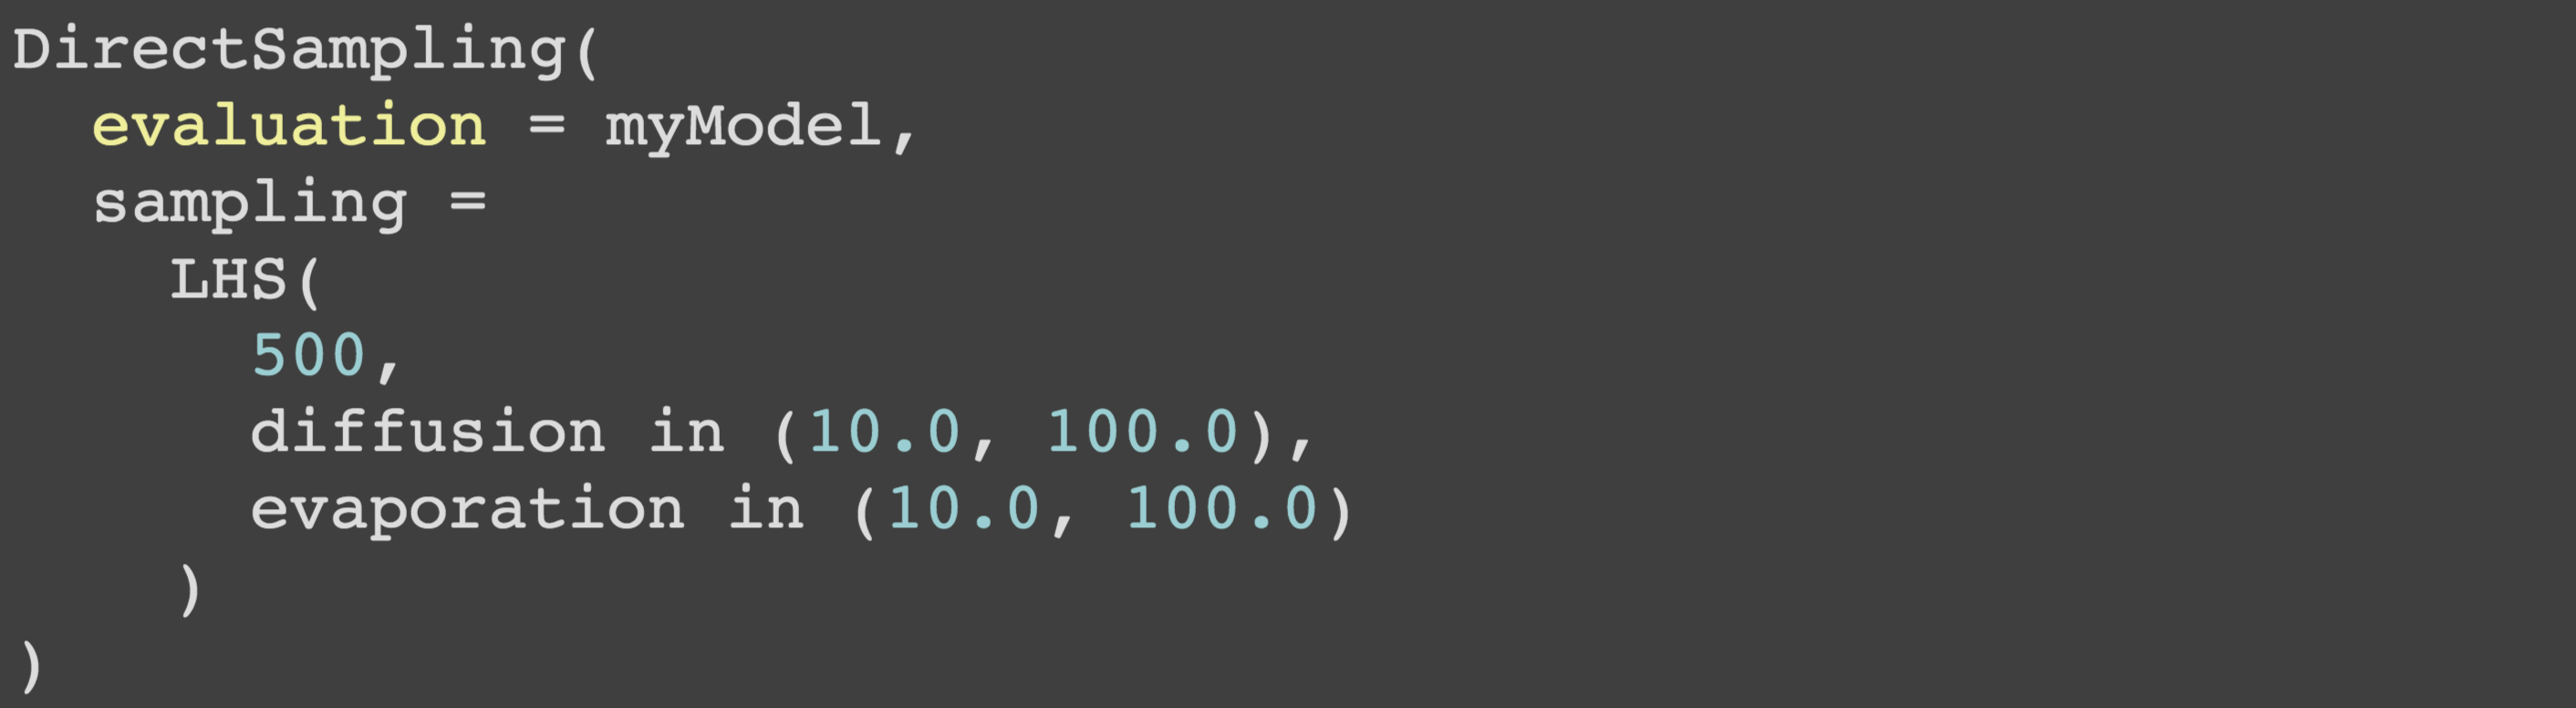
\includegraphics[width=\textwidth]{figures/directsampling.png}
	\end{center}

	\bigskip
	
	Exemple de syntaxe d'une méthode : échantillonnage explicite

}




\sframe{Environnements de calcul: passage à l'échelle}{

% Prototype Small, Scale for Free

% Zero deployment approach
% No prior knowledge of remote environment needed
% No installation required on any machine
% User code and data are automatically deployed

\textit{Prototypes locaux, passage à l'échelle transparent: zero déploiement, pas de connaissance technique requise, pas d'installation préalable.}

\bigskip

	\centering
	
	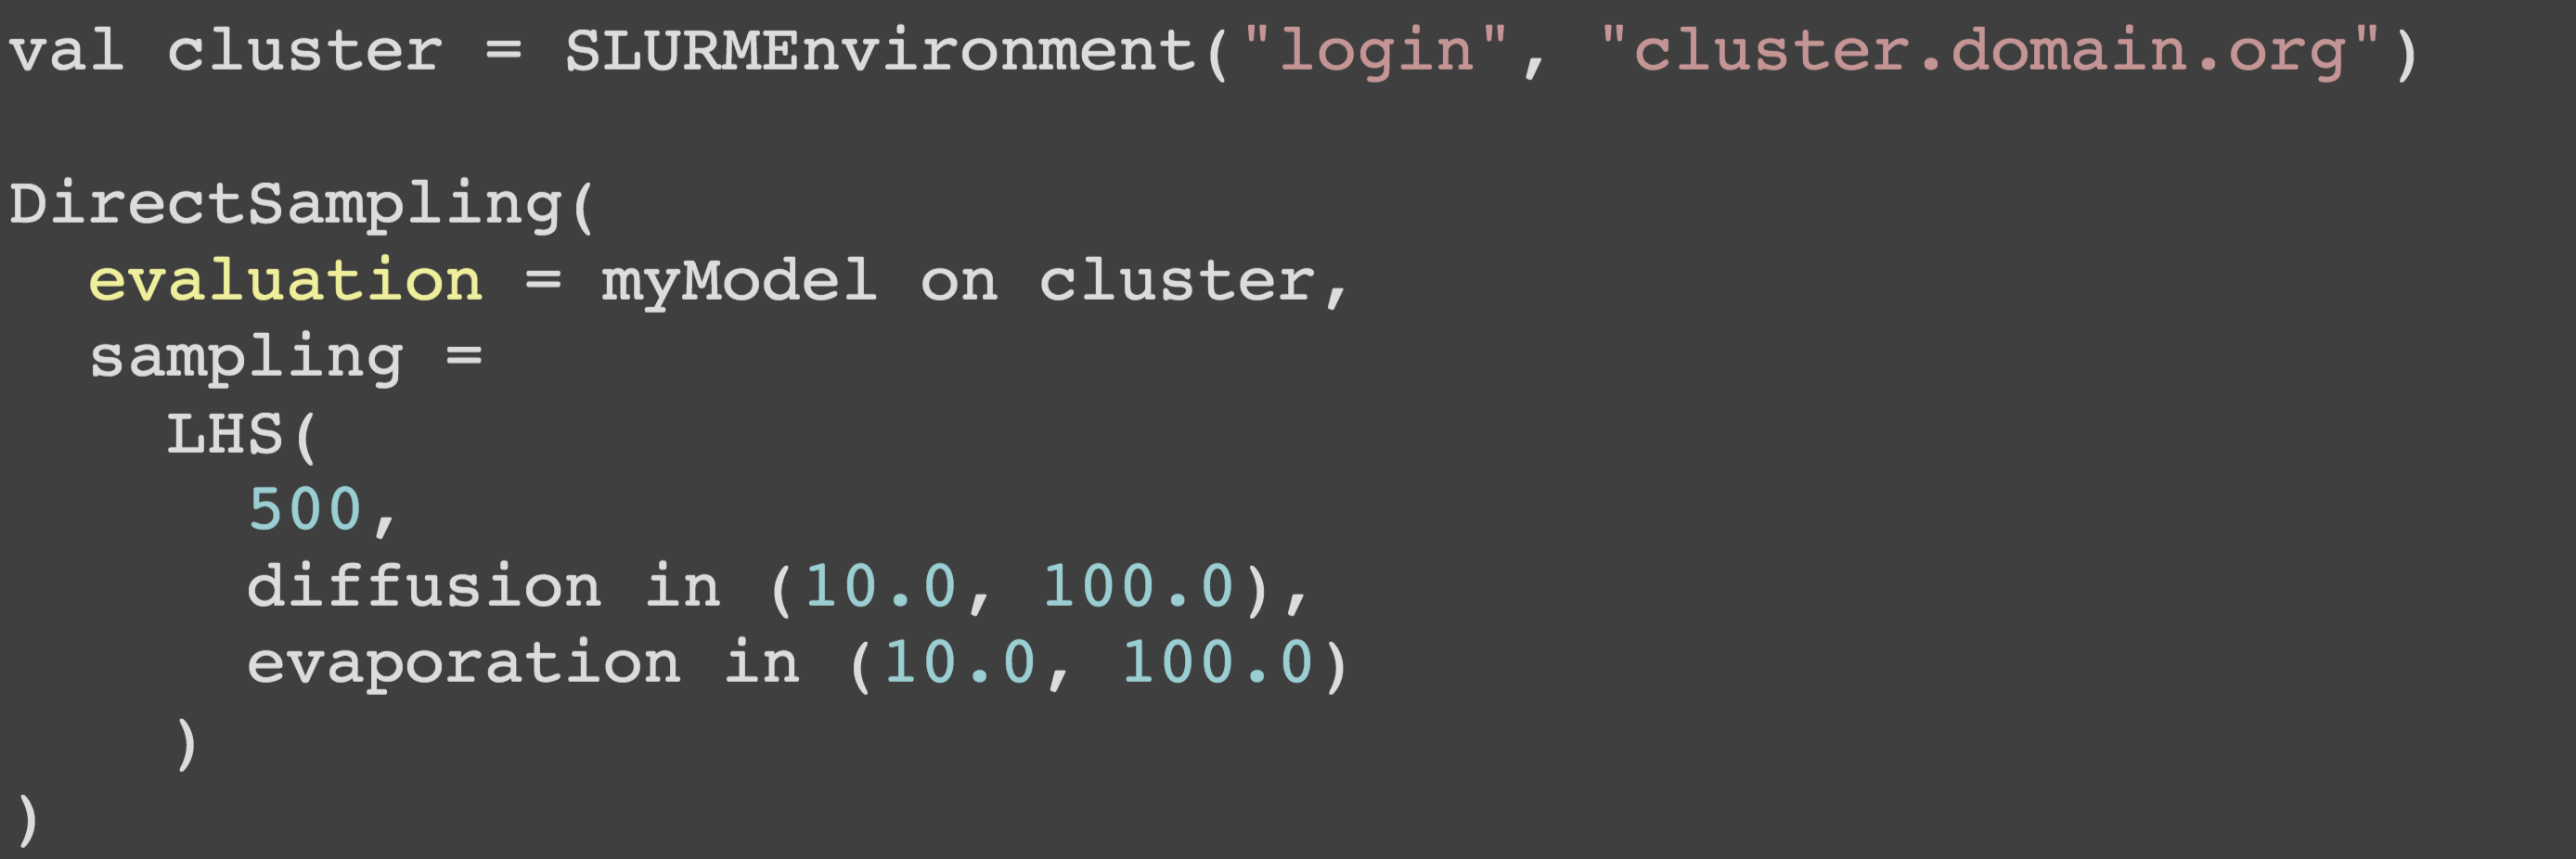
\includegraphics[width=\textwidth]{figures/cluster.png}

}

\sframe{Environnements supportés}{

\textit{Environnements de calcul disponibles :}

\medskip

\begin{itemize}
	\item Multi-thread
	\item Delegation through SSH
	\item PBS
	\item SLURM
	\item Condor
	\item SGE
	\item OAR
	\item EGI Grid
\end{itemize}



}


\sframe{Rôle des méthodes dans le processus de modélisation}{

%Computer assisted modeling
%Build a general framework and algorithms to guide the modeling process.

\textit{Cadre théorique et méthodes (algorithmes) pour accompagner le processus de modélisation}

\bigskip

Un processus de modélisation:

\medskip

\begin{enumerate}
	\item Traçable: comprendre les choix effectués
	\item Reproductible: vérification des raisons de ceux-ci
	\item Réutilisable: étudier des choix alternatifs
\end{enumerate}

%traceable: understand what choices were made,
%reproducible: recompute the reason why they were made,
%reusable: study alternative choices.

}


\sframe{Evaluation des modèles et théories}{

	{\centering
	
	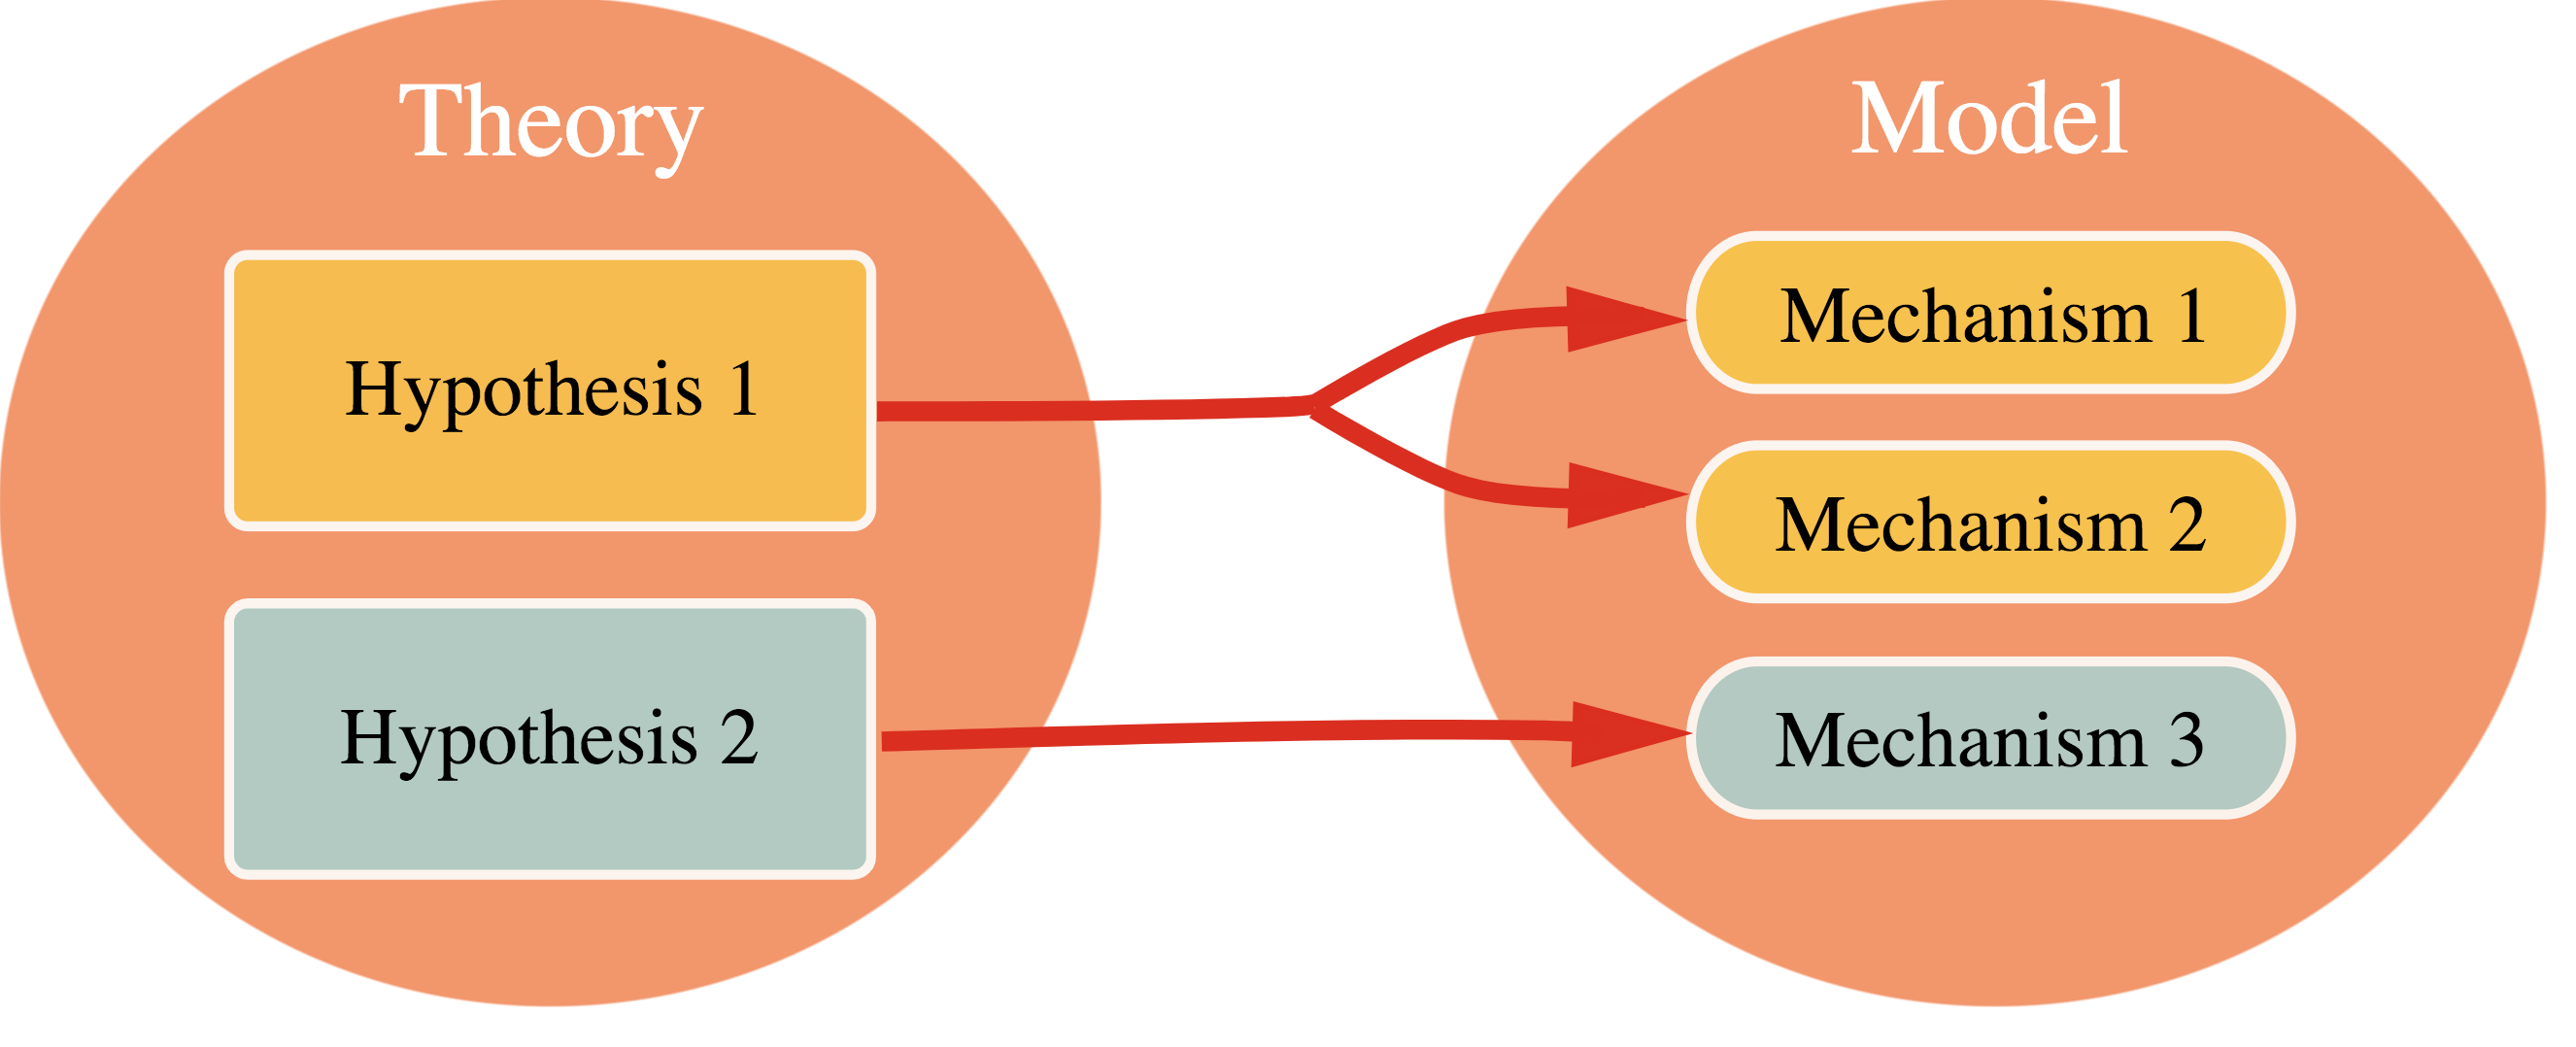
\includegraphics[width=\textwidth]{figures/descriptivemodel.png}
}

%Descriptive models
%Design/evaluate a theory involving causal effects through its capacity to (re-)produce some patterns/data.

\textit{Construire et évaluer une théorie impliquant des effets causaux par sa capacité à (re-)produire des motifs ou données.}


\medskip

%Model evaluation
%How to assess:

\textbf{Evaluation: } Comment s'assurer de

\begin{enumerate}
	\item La suffisance des mécanismes ?
	\item La nécessité des mécanismes ?
	\item L'unicité des mécanismes ?
\end{enumerate}
%the sufficiency of the mechanisms ?
%the necessity of the mechanisms ?
%the uniqueness of the mechanisms ?


}




\sframe{Suffisance \cite{schmitt2014half}}{

Approche classique: échantillonnage (ex. Sobol) $\rightarrow$ énorme quantité de données produites; le problème devient une question de fouille de données; espace des paramètres laissé majoritairement inexploré.

\bigskip

\textit{Approche inverse: des sorties aux paramètres}

\medskip

%Formalising the expectations
\textit{Formalisation thématique d'indicateurs: }

	\begin{center}
	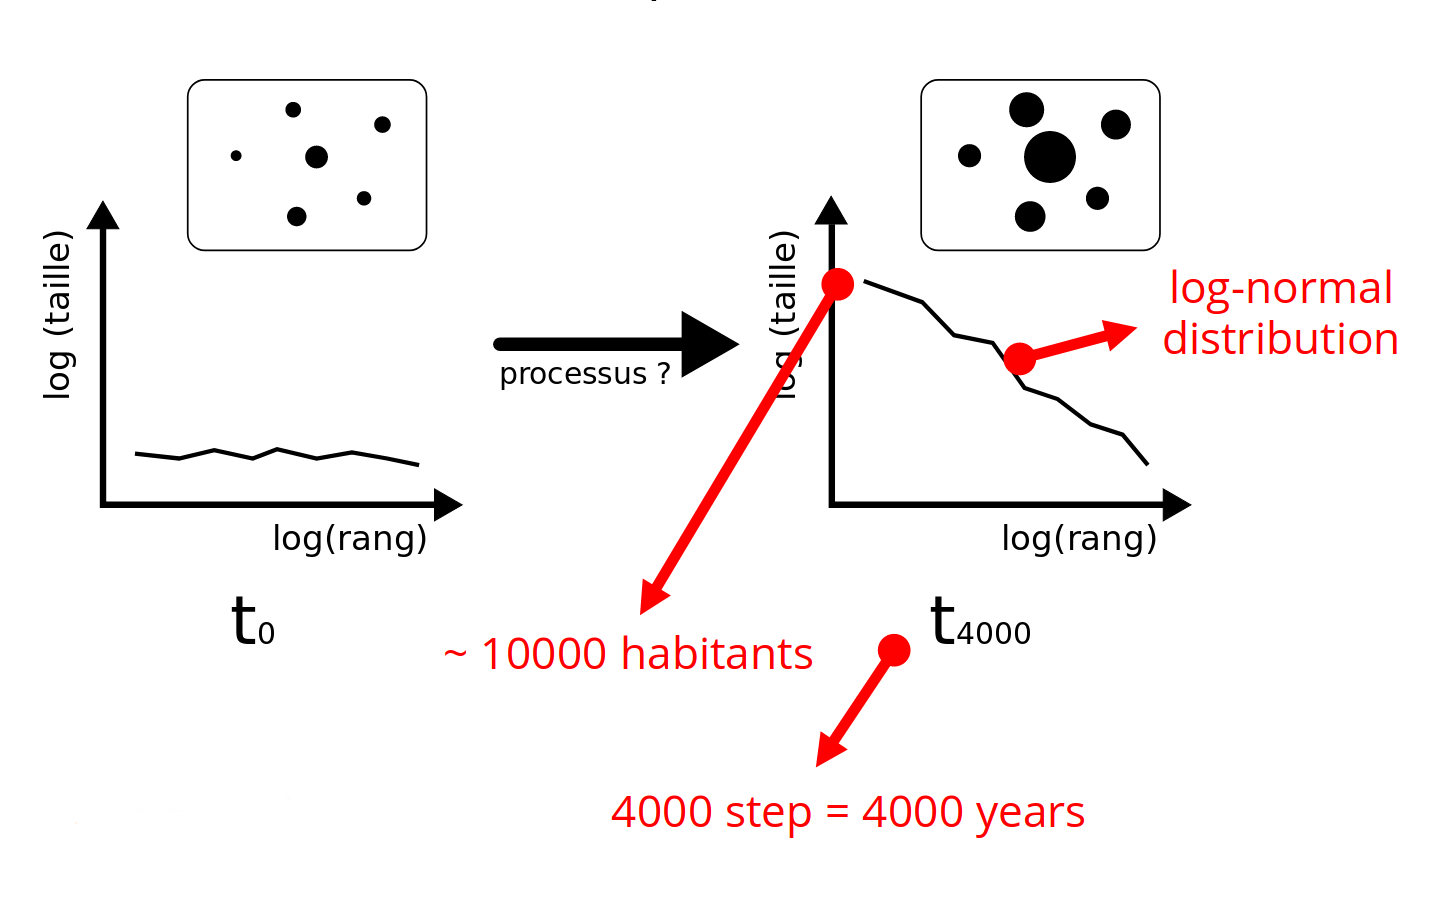
\includegraphics[width=\textwidth]{figures/slocal_fitness.png}
	\end{center}

\bigskip

$\rightarrow$ minimisation multi-objectifs par un algorithme génétique NSGA2	
	

}




\sframe{Résultats de calibration}{
	
	%No compromise between the 3 objectives.
	\textit{Pas de compromis entre les trois objectifs.}

\medskip

	{\centering
	
	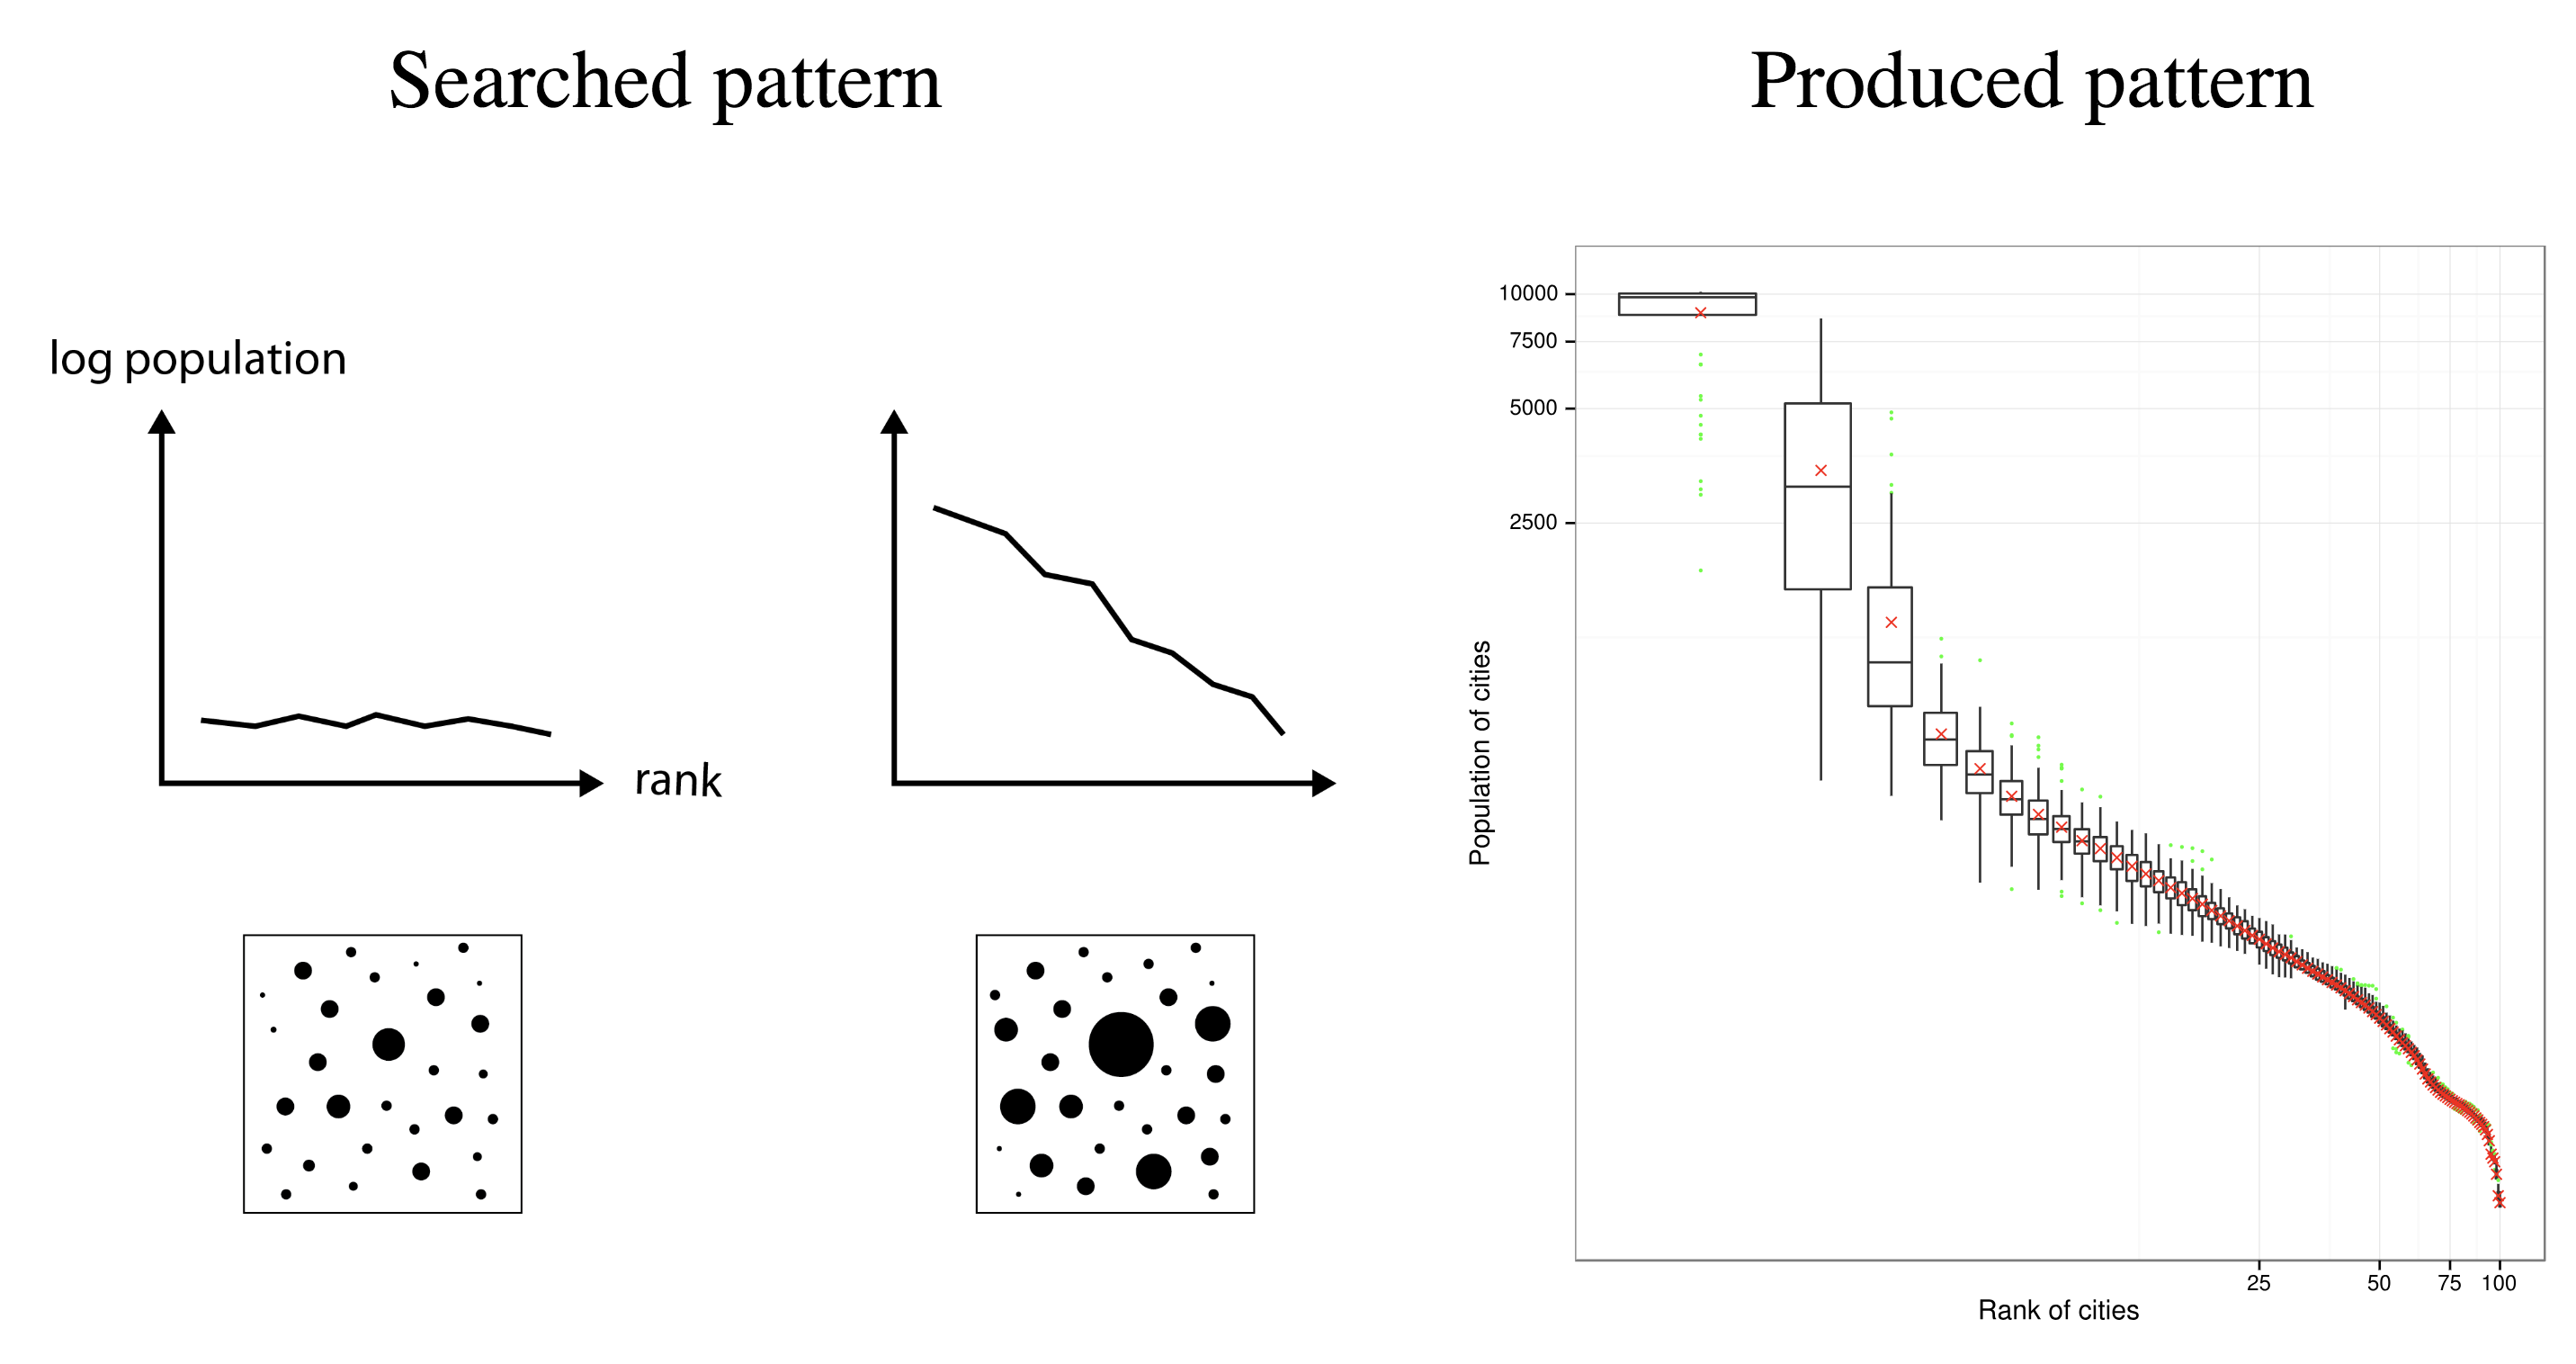
\includegraphics[width=\textwidth]{figures/slocalcalib.png}
	}
	
%	Evaluation approach
%Would not have been found using a direct method.


%The method is tractable (even for ABMs):
%Handles stochasticity: 100x gain.
%Support for distributed computing: 1000x gain.

\medskip

Performances: gestion de la stochasticité (gain x100), calcul distribué (gain x1000)


%Conclusion
%How to assess:

%the sufficiency of the mechanisms Y
%the necessity of the mechanisms ?
%the uniqueness of the mechanisms ?

}


\sframe{Nécessité \cite{reuillon2015}}{

%A new algorithm
%To detect if a parameter is useful: it impacts the capacity of the model to produce plausible outcomes.

%To better constrain the parameter ranges.
%As an indirect way to detect if some of the mechanisms are expandable

\textbf{Nouvel algorithme}

\medskip

\begin{enumerate}
	\item Détecte si un paramètre est nécessaire
	\item Contraint mieux les bornes des paramètres
	\item Façon indirecte d'identifier des extensions possibles
\end{enumerate}


%Objective
%Hundreds of calibrations

	%\centering
	
	%\includegraphics[width=\textwidth]{figures/PdiffusionZ.pdf.png}


}

\sframe{Algorithme des profils}{
{\centering
	
	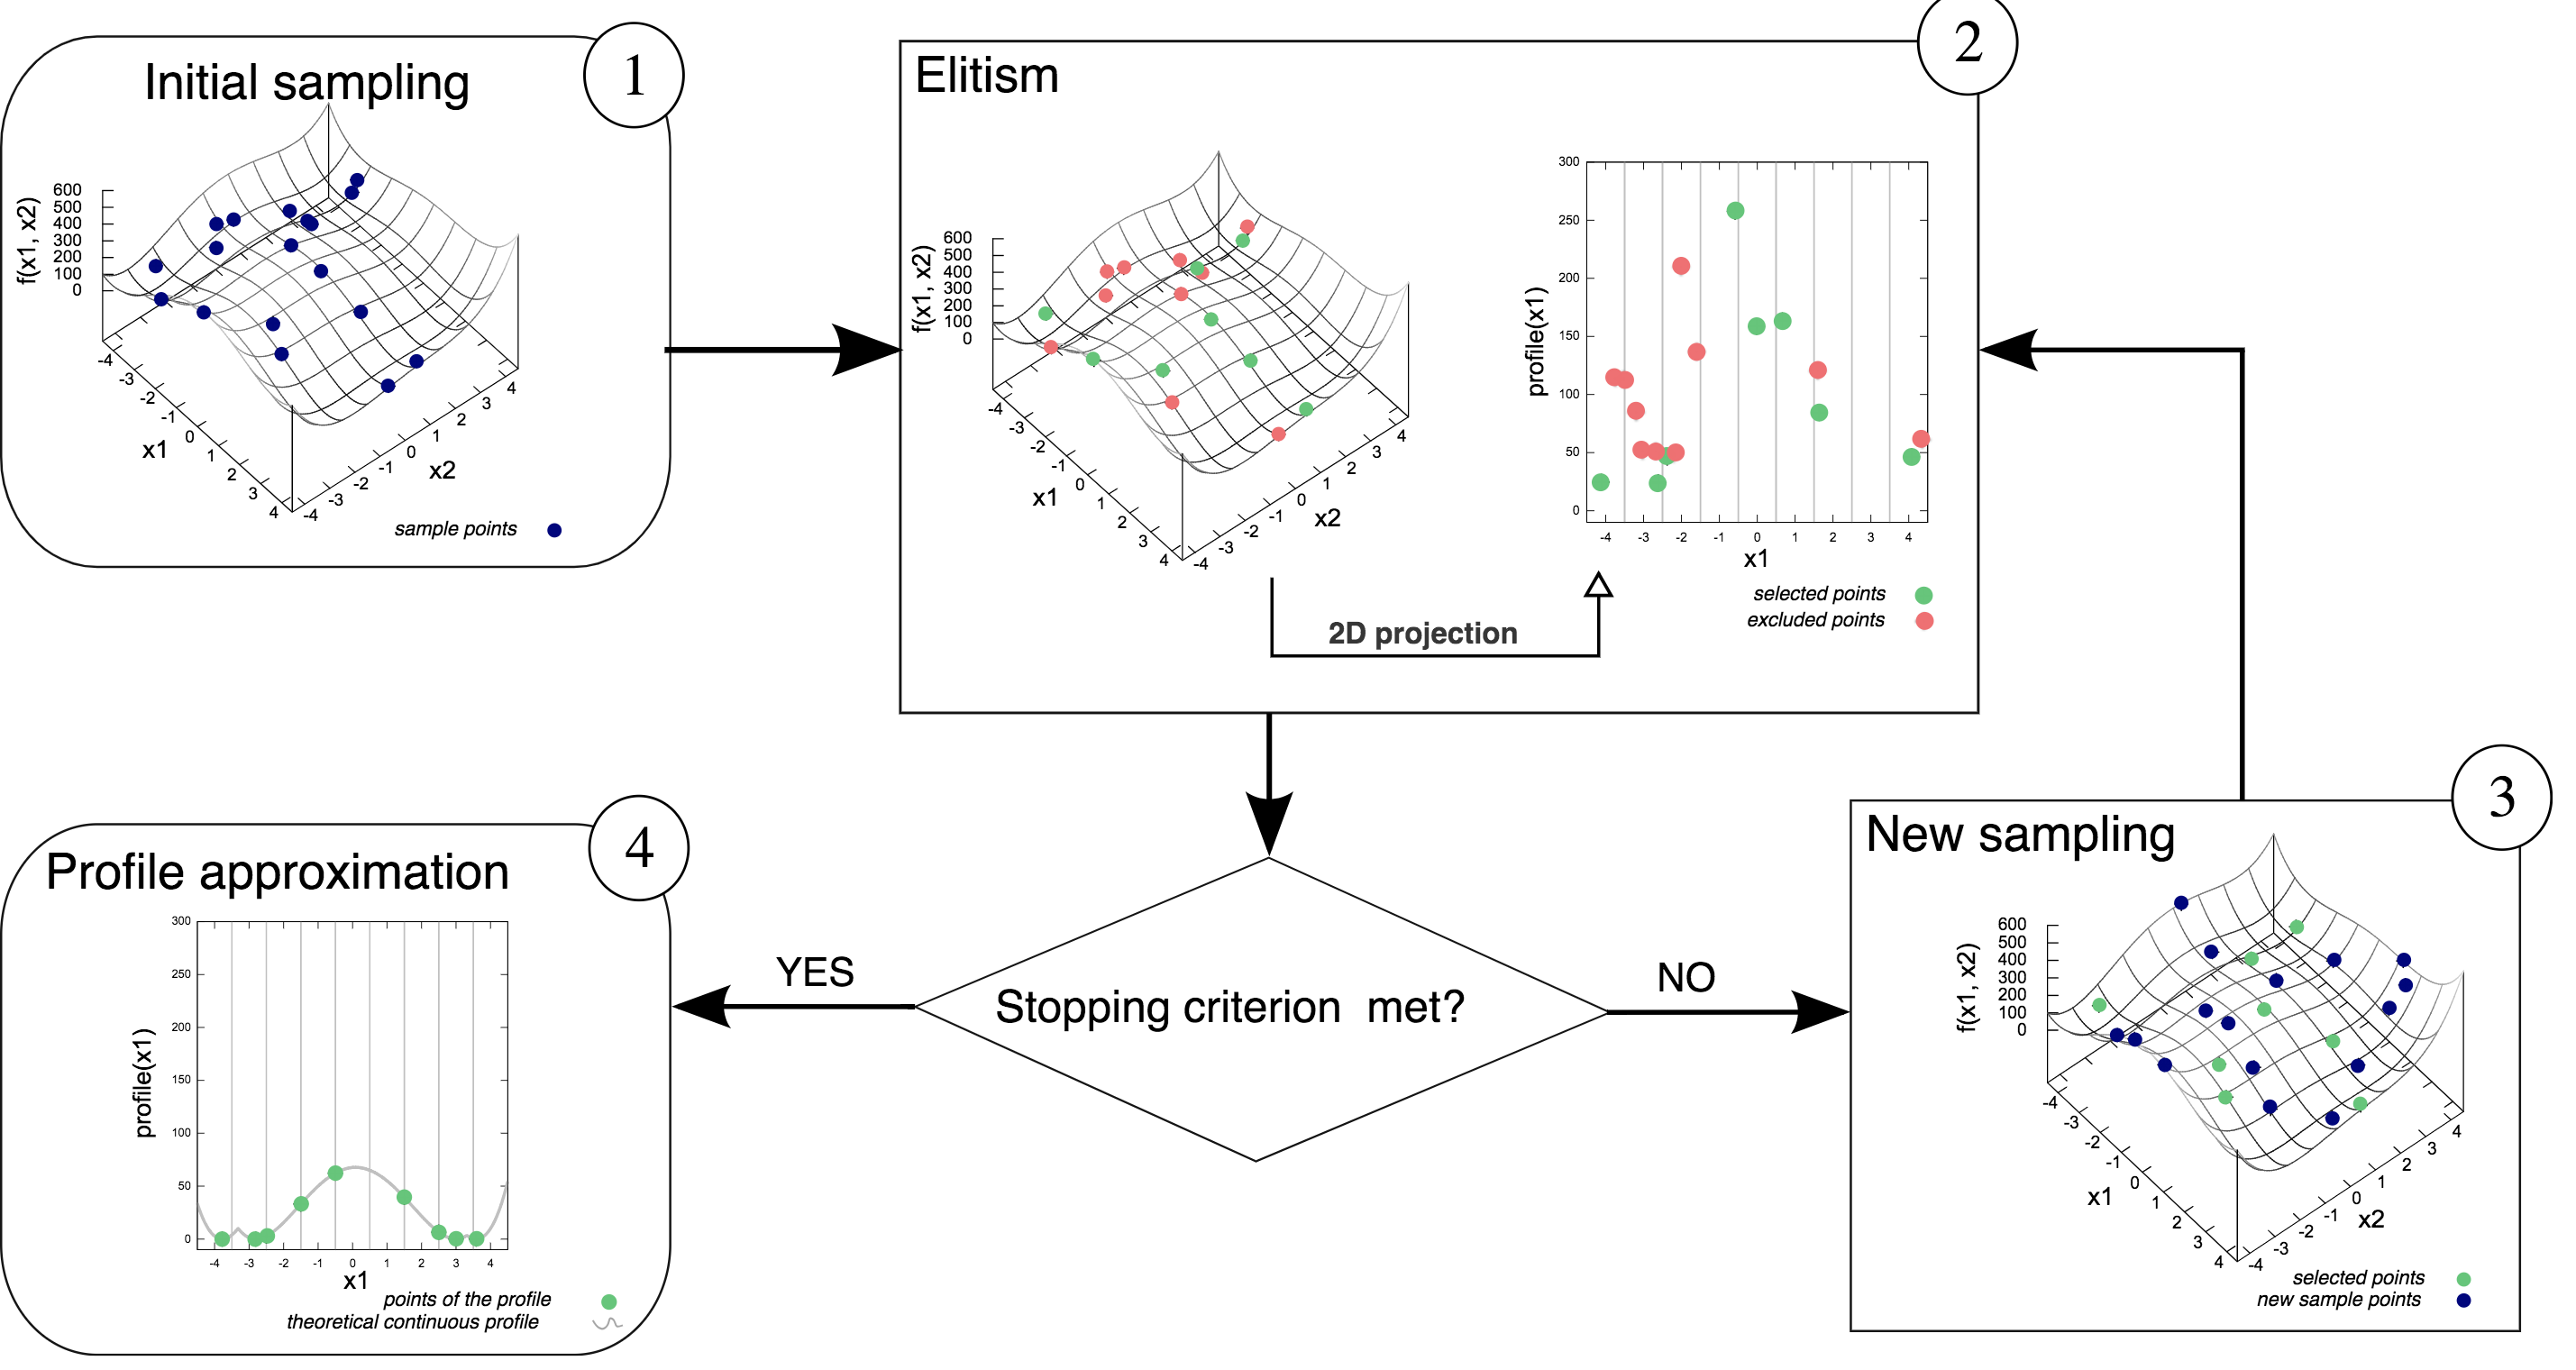
\includegraphics[width=\textwidth]{figures/profil_algo.png}
}
	
%The profile algorithm
%Compute the best of calibration for hundreds of values along the definition domain of a parameter.
\medskip
\textit{Meilleure calibration pour des pas fixés le long d'une dimension}


%The method is tractable (even for ABMs):
%Converges almost as fast a single calibration.
%Handles stochasticity: 100x gain.
%Support for distributed computing: 1000x gain.	
	
}



\sframe{Algorithme des profils}{
\centering
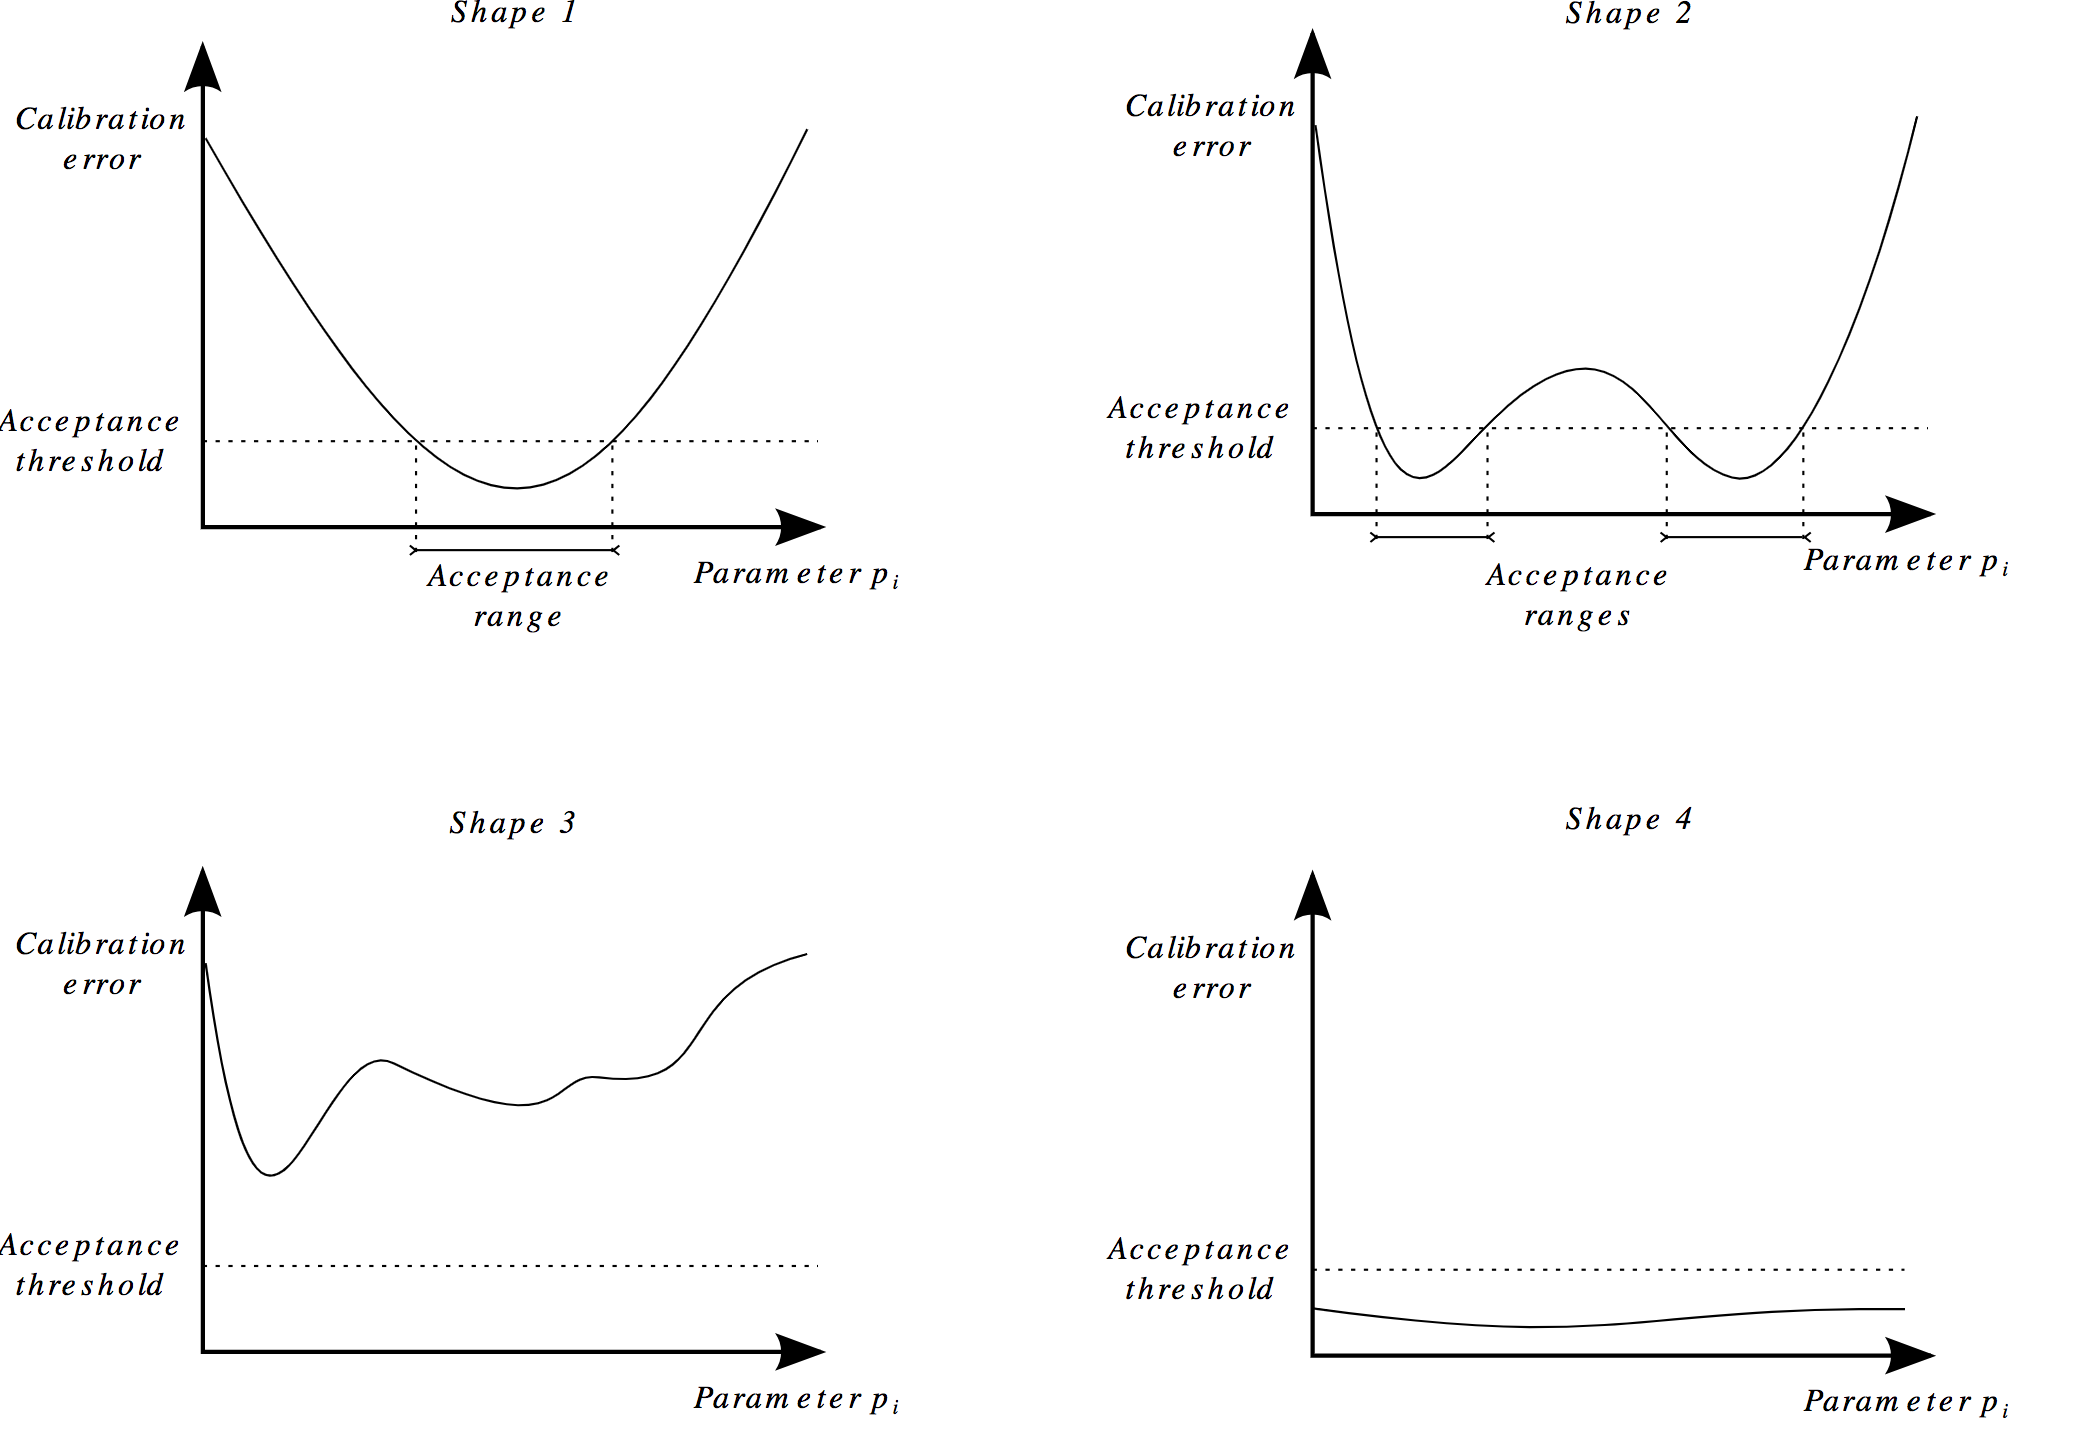
\includegraphics[width=\textwidth]{figures/profil_interpretation.png}
}


\sframe{Résultats}{

	\centering
	
	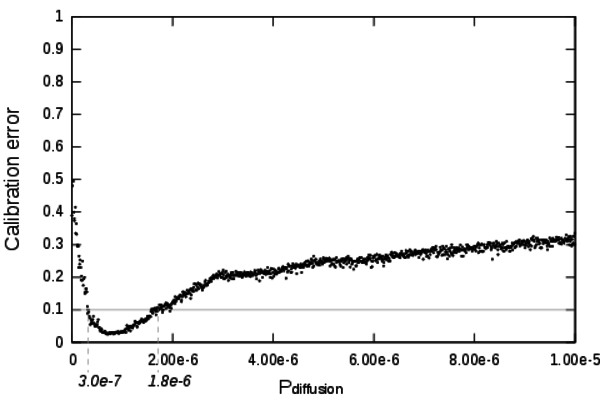
\includegraphics[width=\textwidth]{figures/PdiffusionZ.png}

}

\sframe{Résultats}{

	\centering
	
	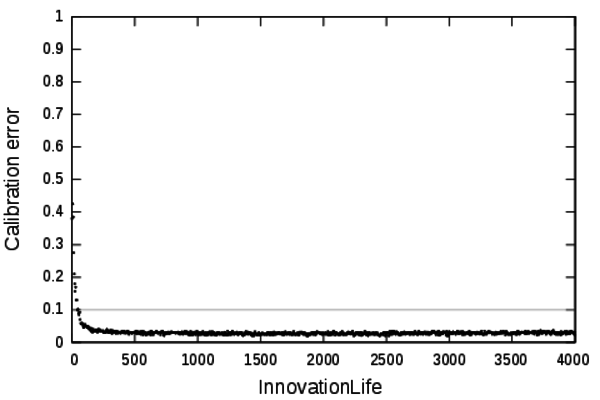
\includegraphics[width=\textwidth]{figures/InnovationLife.png}

%Conclusion
%How to assess:

%the sufficiency of the mechanisms Y
%the necessity of the mechanisms Y
%the uniqueness of the mechanisms ?

}


\sframe{Unicité \cite{cottineau2014evolution}}{

%Automate the confrontation of alternative hypothesis / mechanisms.

\textit{Automatisation de la confrontation entre hypothèses/mécanismes alternatifs}

\medskip

\centering
	
	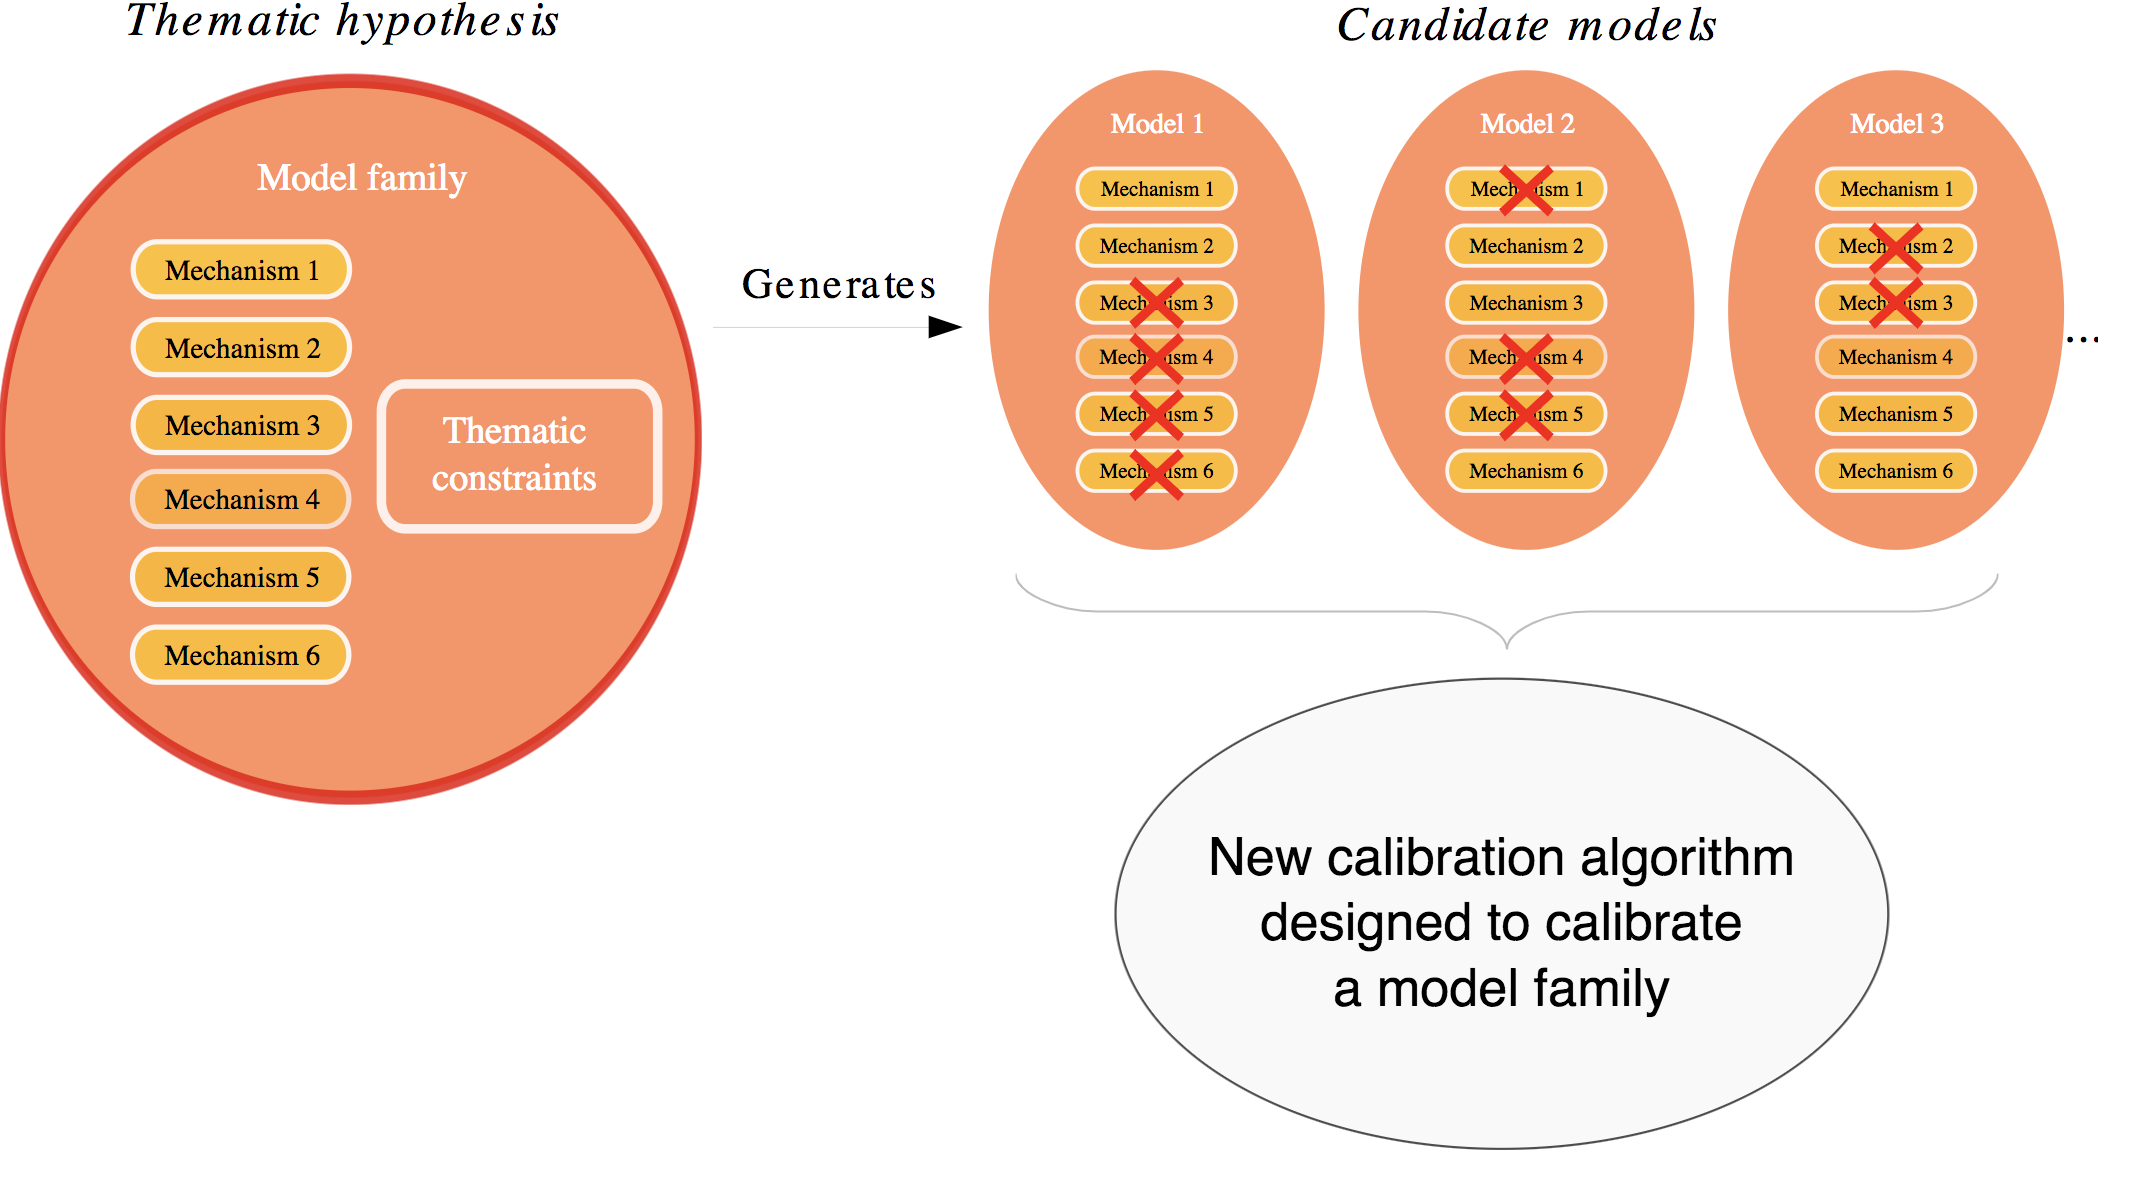
\includegraphics[width=\textwidth]{figures/simfamily.png}

}


\sframe{Objectif}{


%What we are running after?

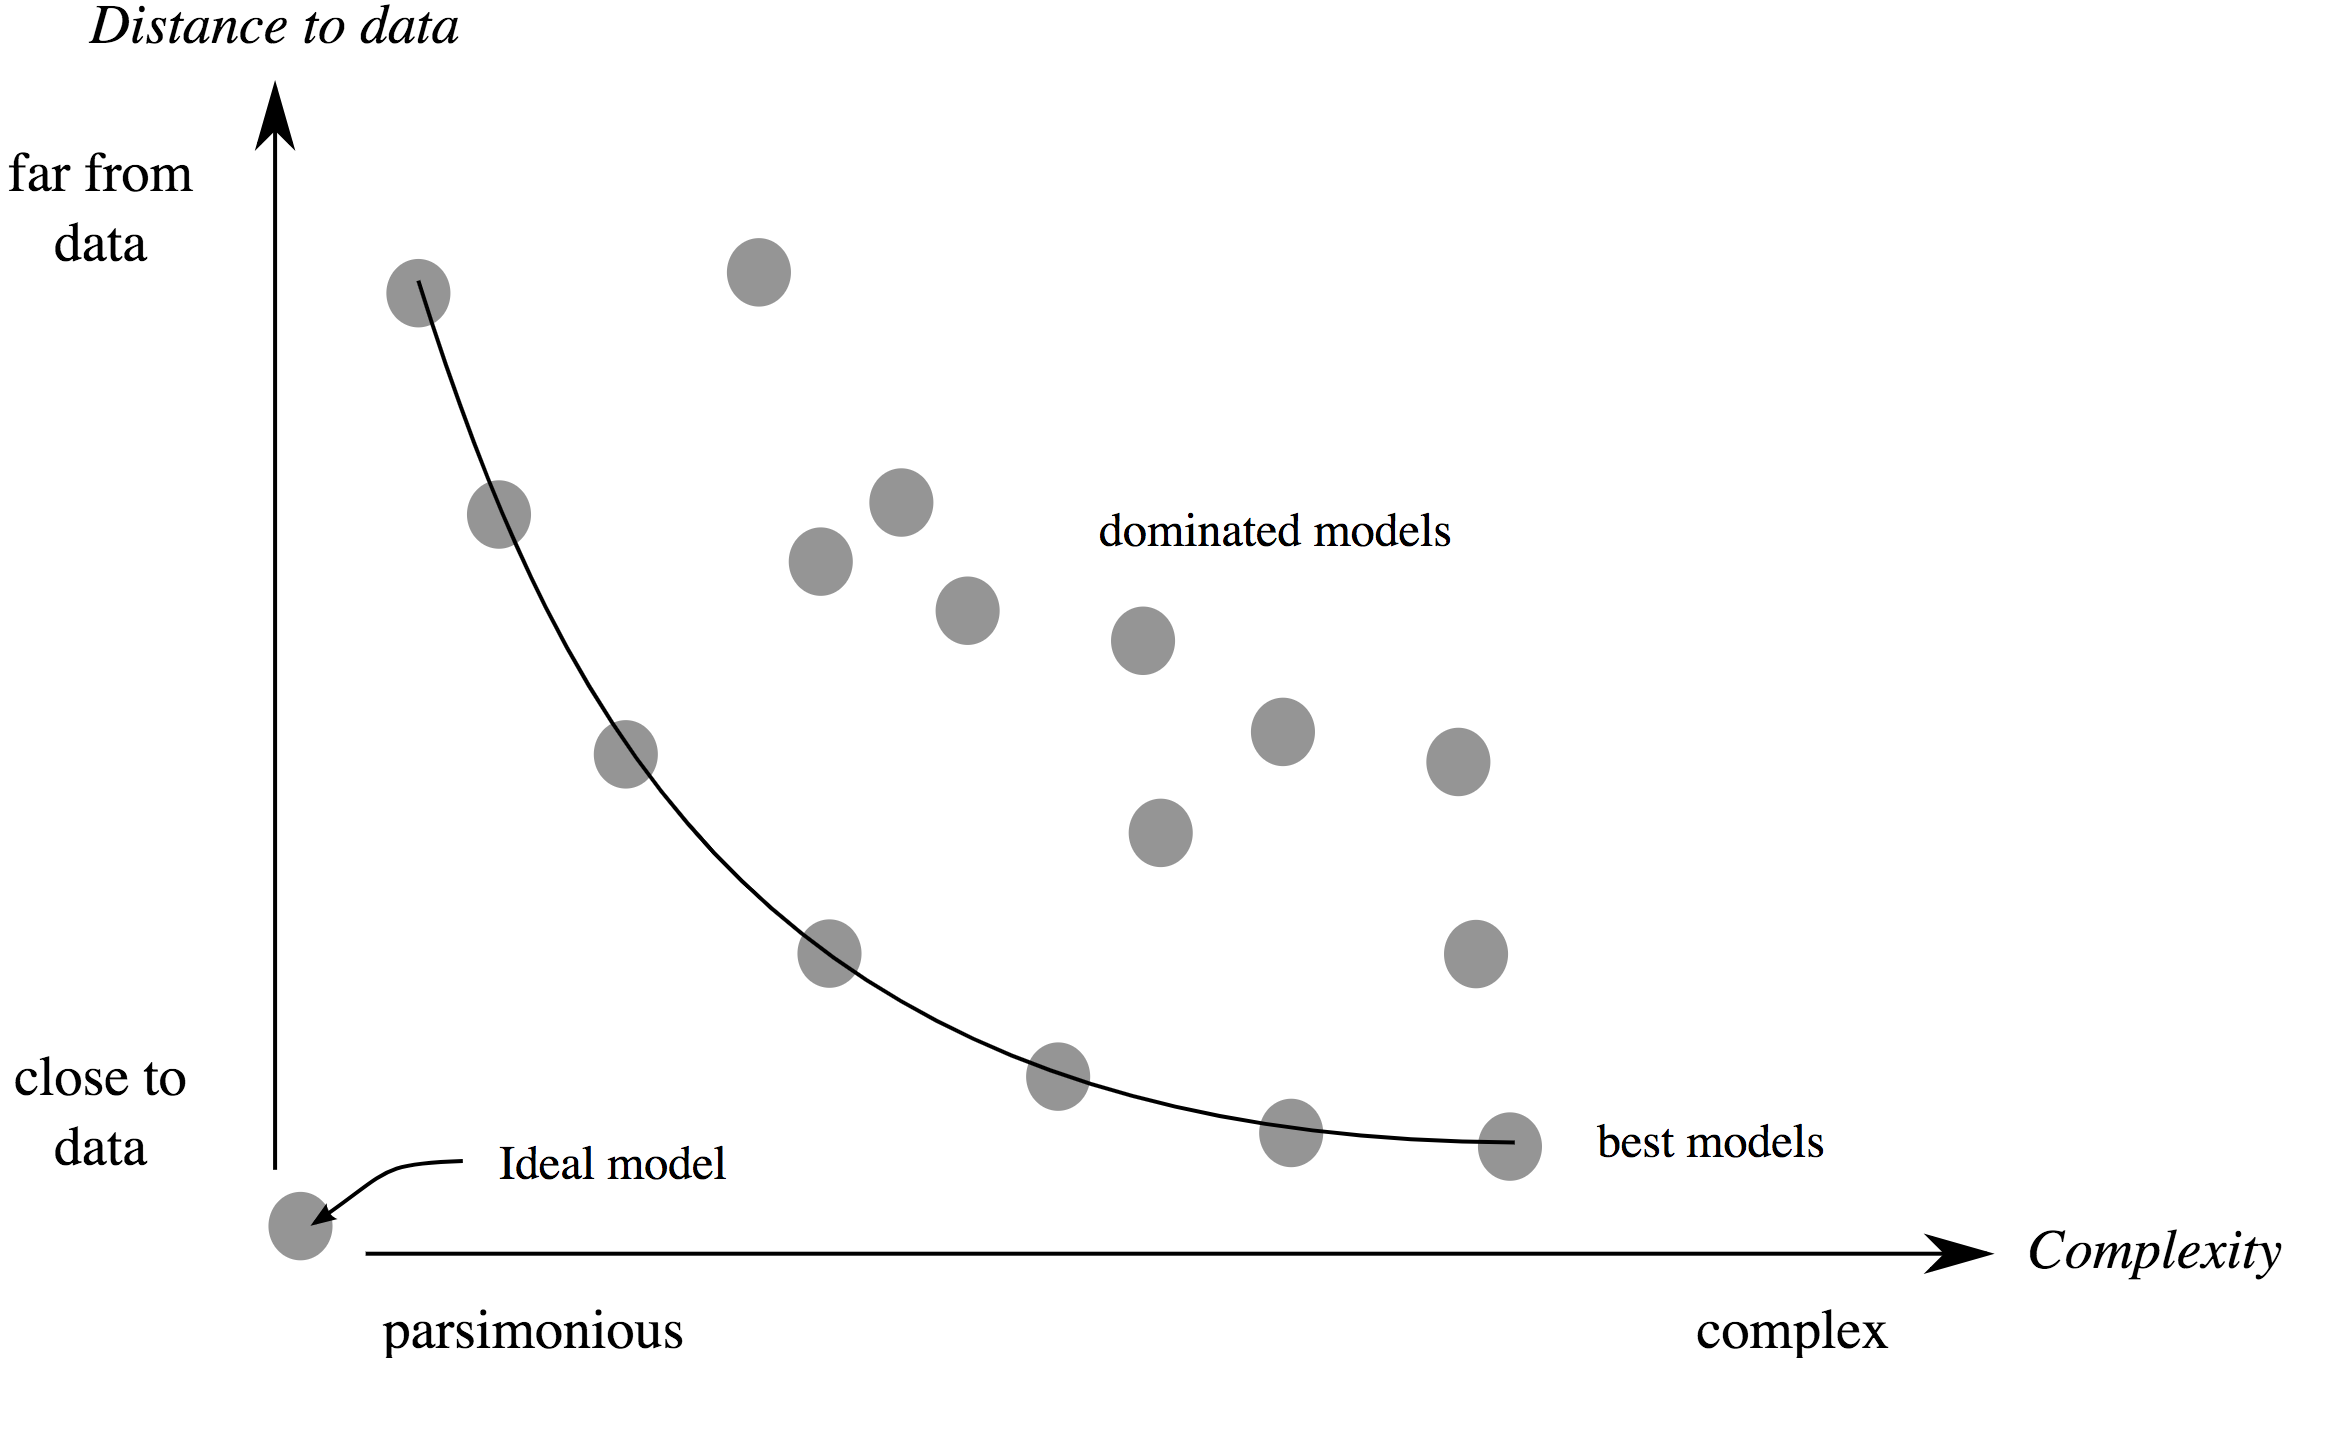
\includegraphics[width=\textwidth]{figures/paretocomplexityfit.png}

}

\sframe{Multi-modélisation (64 modèles)}{

%64 models

\centering

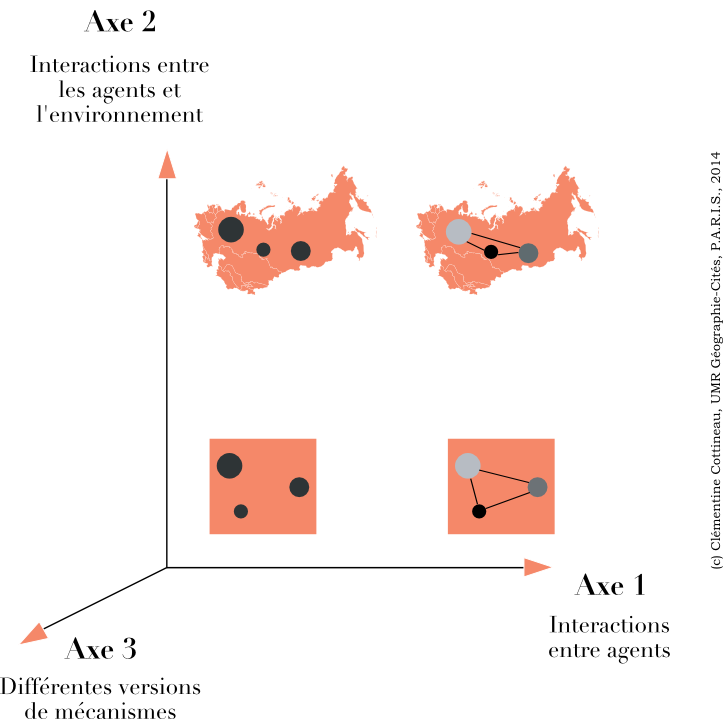
\includegraphics[width=0.8\textwidth]{figures/marius_complexification.png}

}



\sframe{Calibration de la famille de modèles}{

%Compute the best set of parameters for all 64 models.
\textit{Meilleur jeu de paramètres pour l'ensemble des 64 modèles obtenu par un algorithme NSGA2 par niches}

\bigskip

\centering

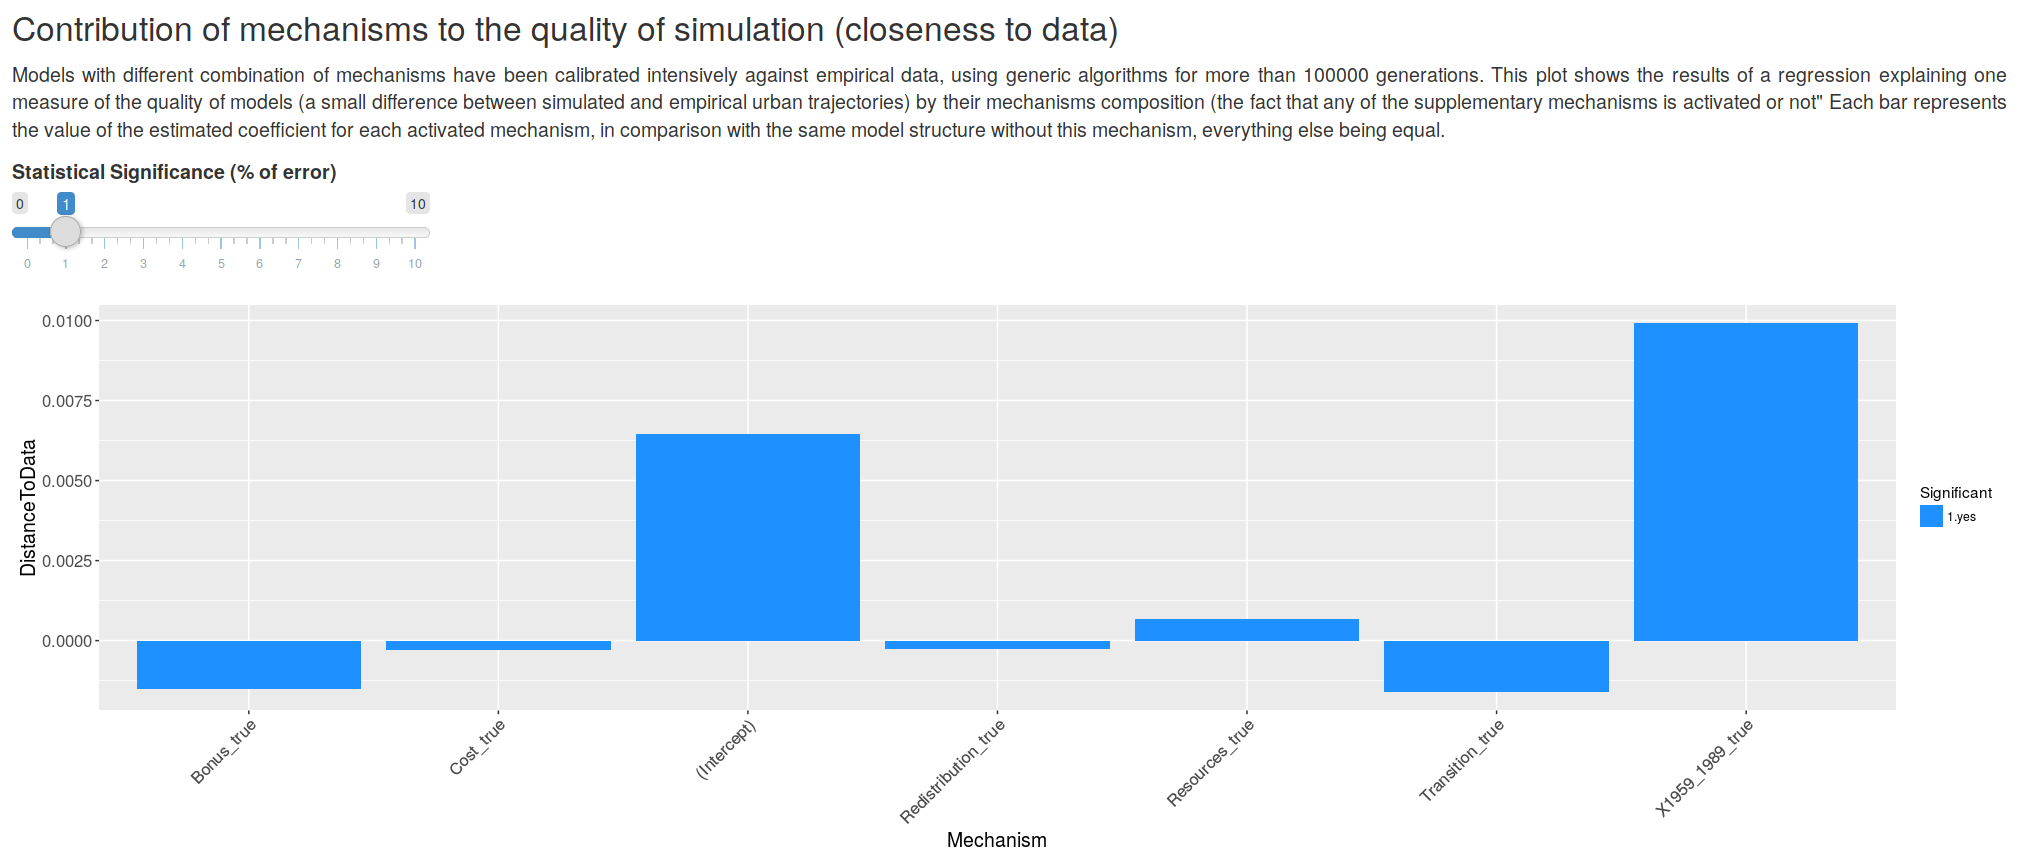
\includegraphics[width=\textwidth]{figures/varius_big.png}


}





\sframe{Recherche de motifs \cite{10.1371/journal.pone.0138212}}{

\centering

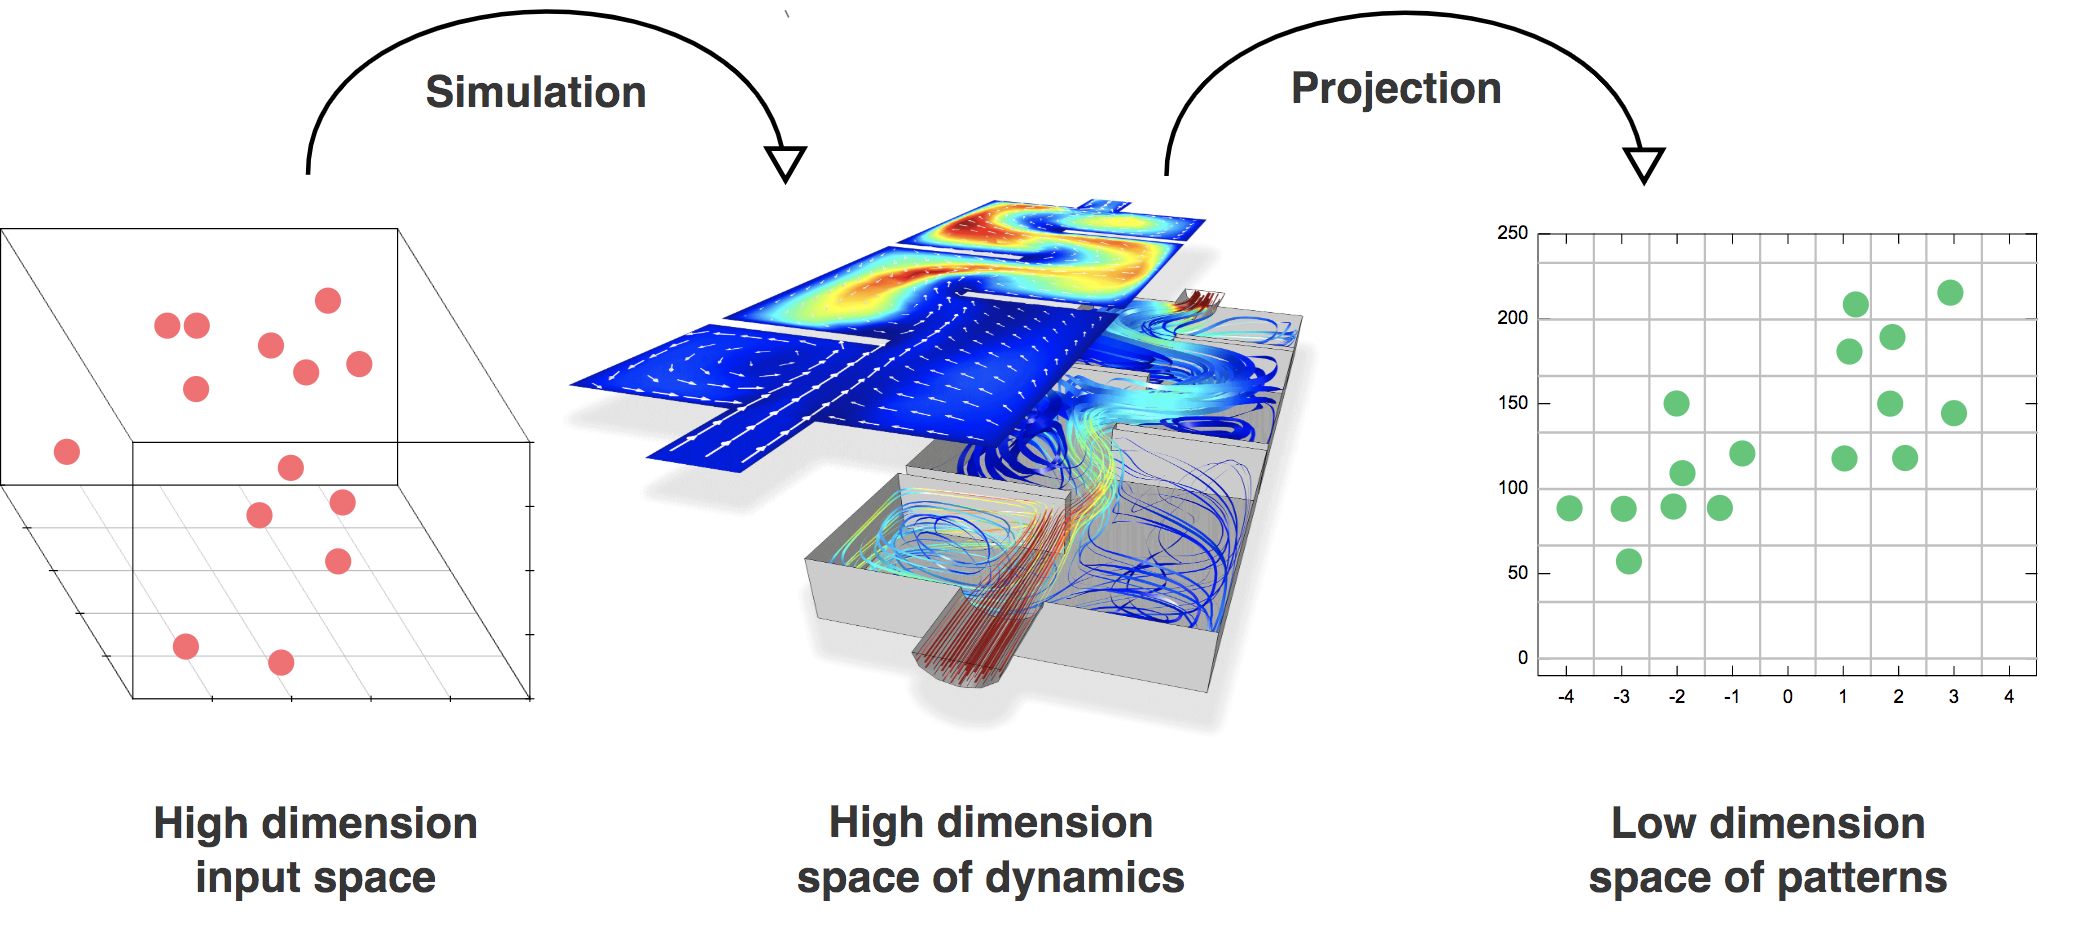
\includegraphics[width=\textwidth]{figures/pse_algo.png}

}

\sframe{Recherche de nouveauté}{

%The inputs producing rare patterns have high fitness values.

\textit{Entrées produisant des motifs rares ont une forte fitness}

\centering

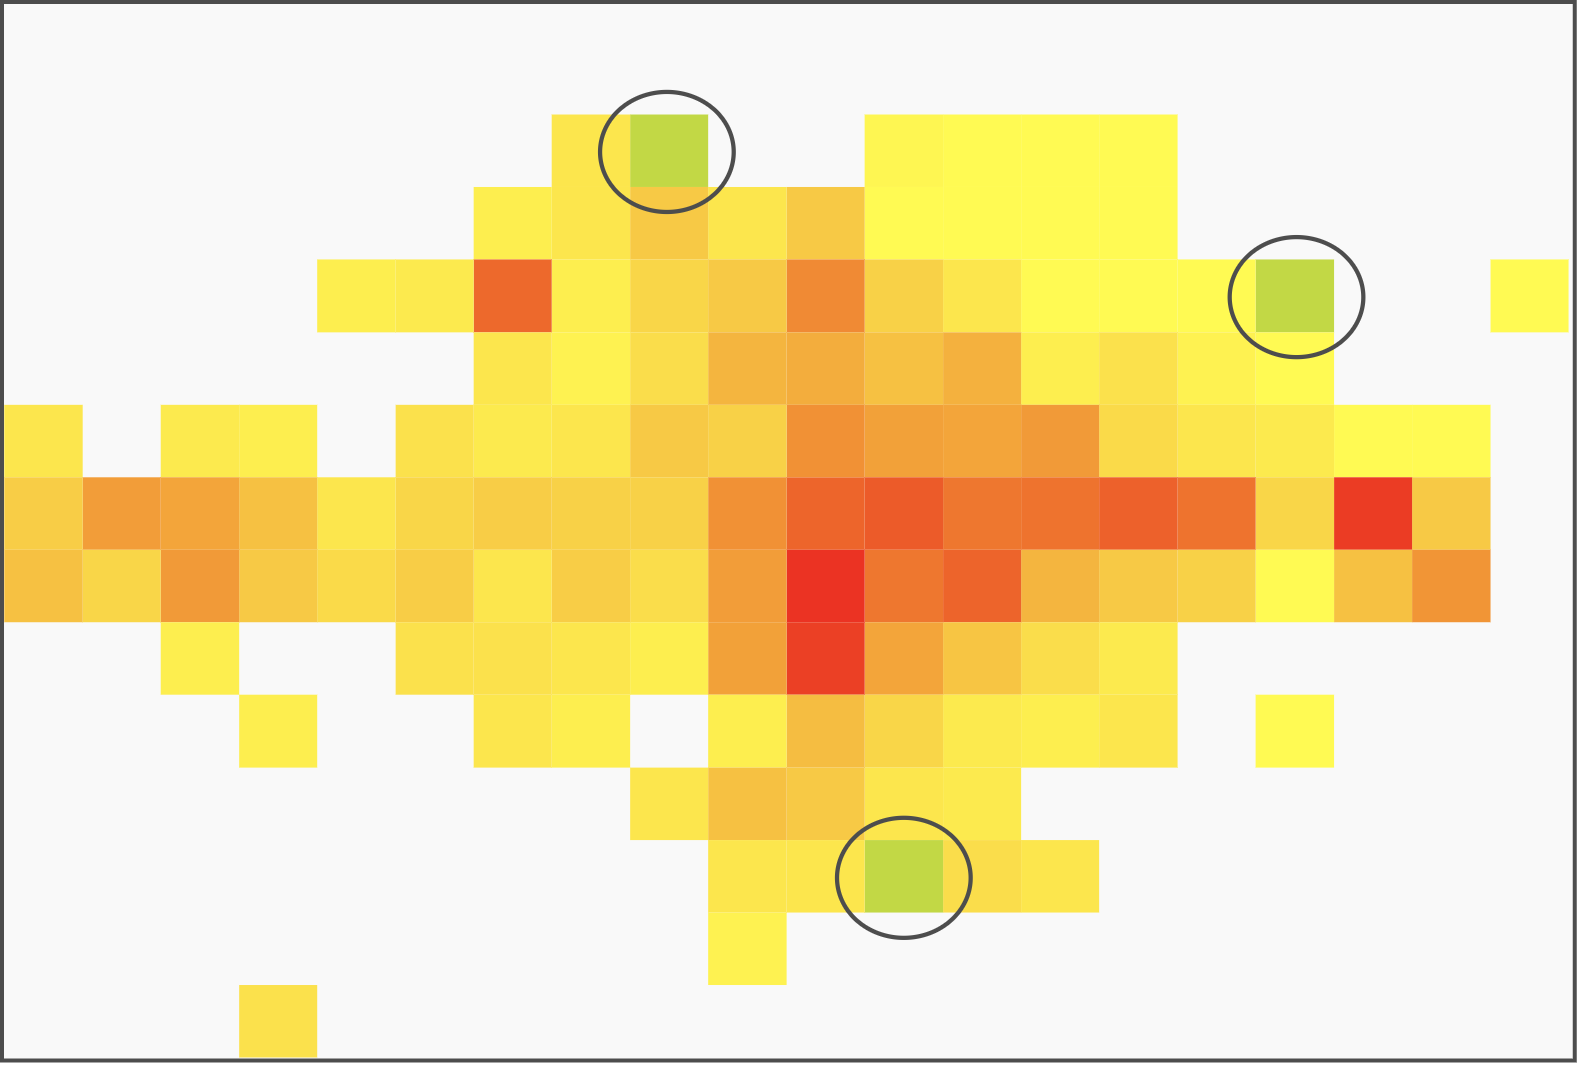
\includegraphics[width=0.9\textwidth]{figures/hitmap.png}

}


\sframe{Résultats}{

\centering

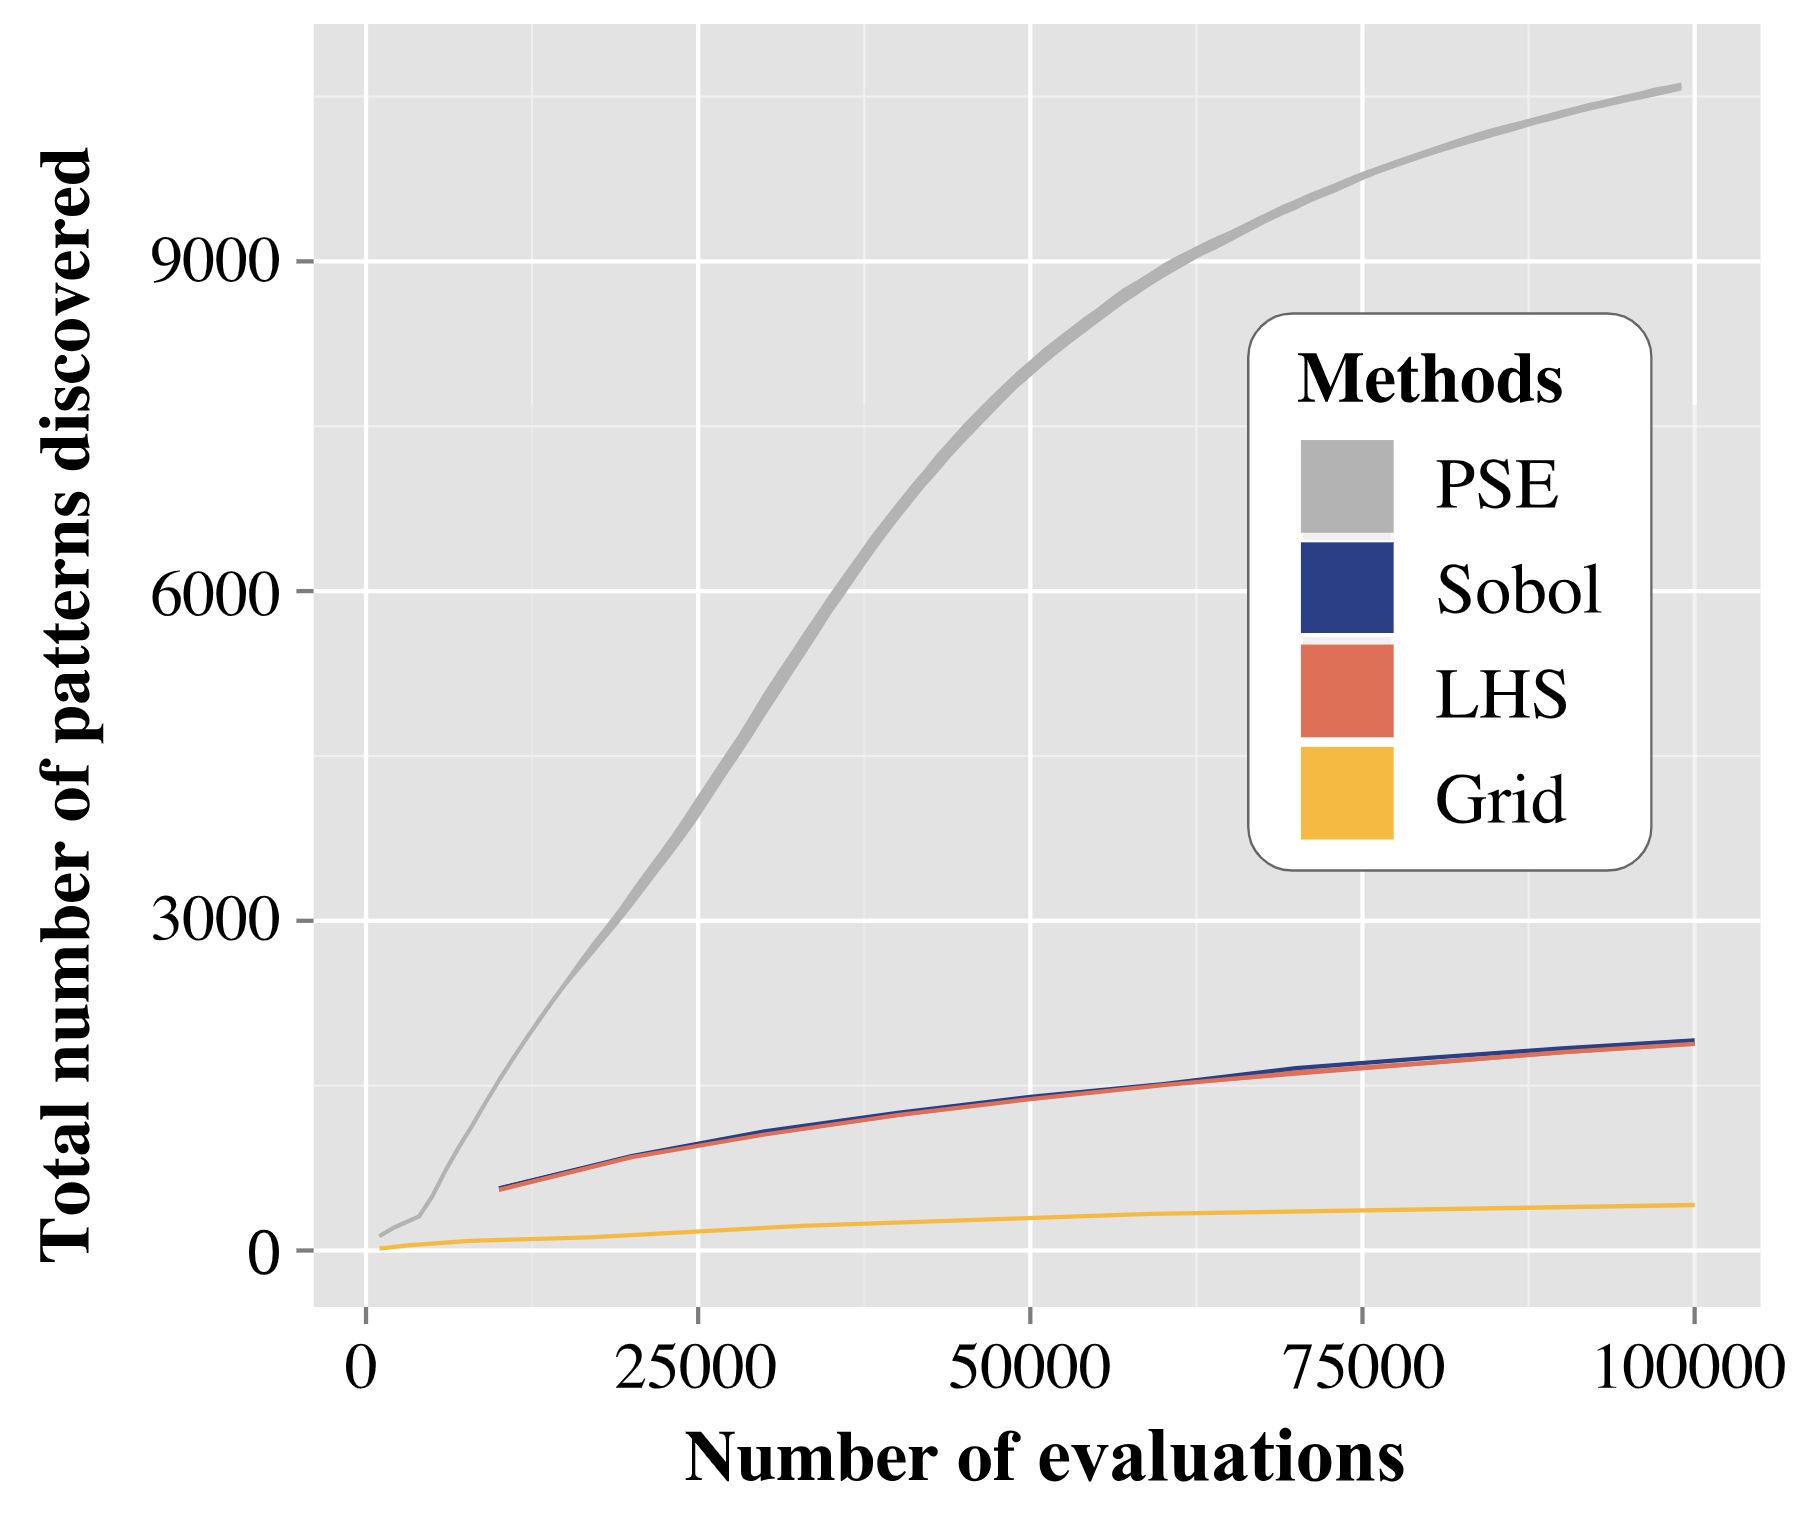
\includegraphics[width=0.9\textwidth]{figures/flockingvolume.png}

}

\sframe{Résultats}{

\centering

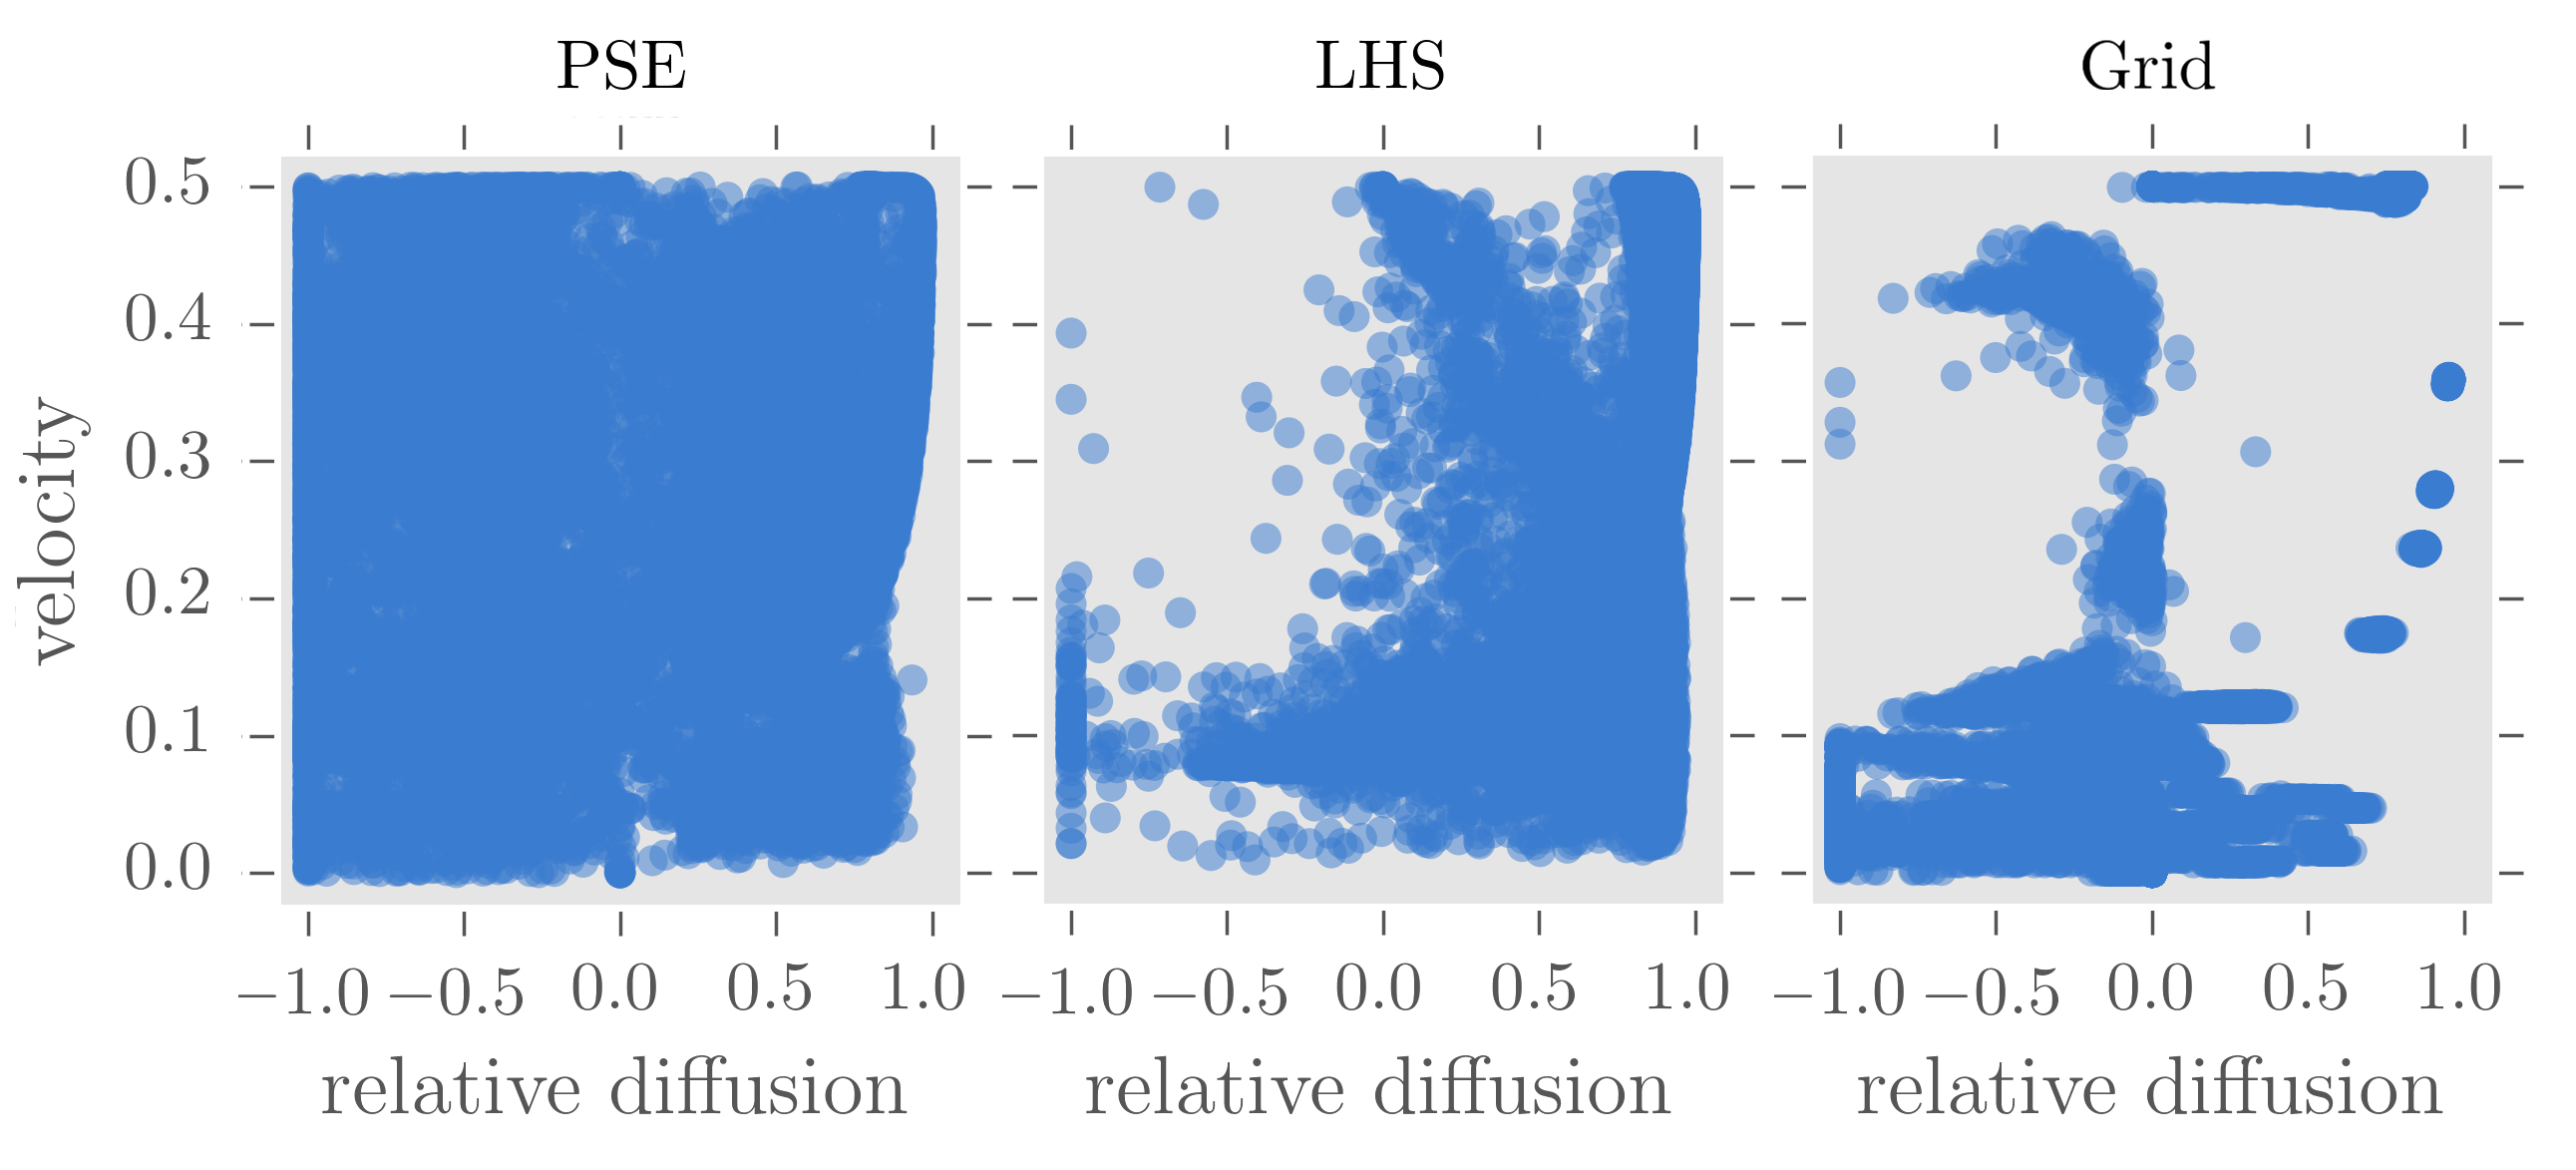
\includegraphics[width=\textwidth]{figures/flockingpatterns.png}

}

\sframe{Résultats}{

\centering

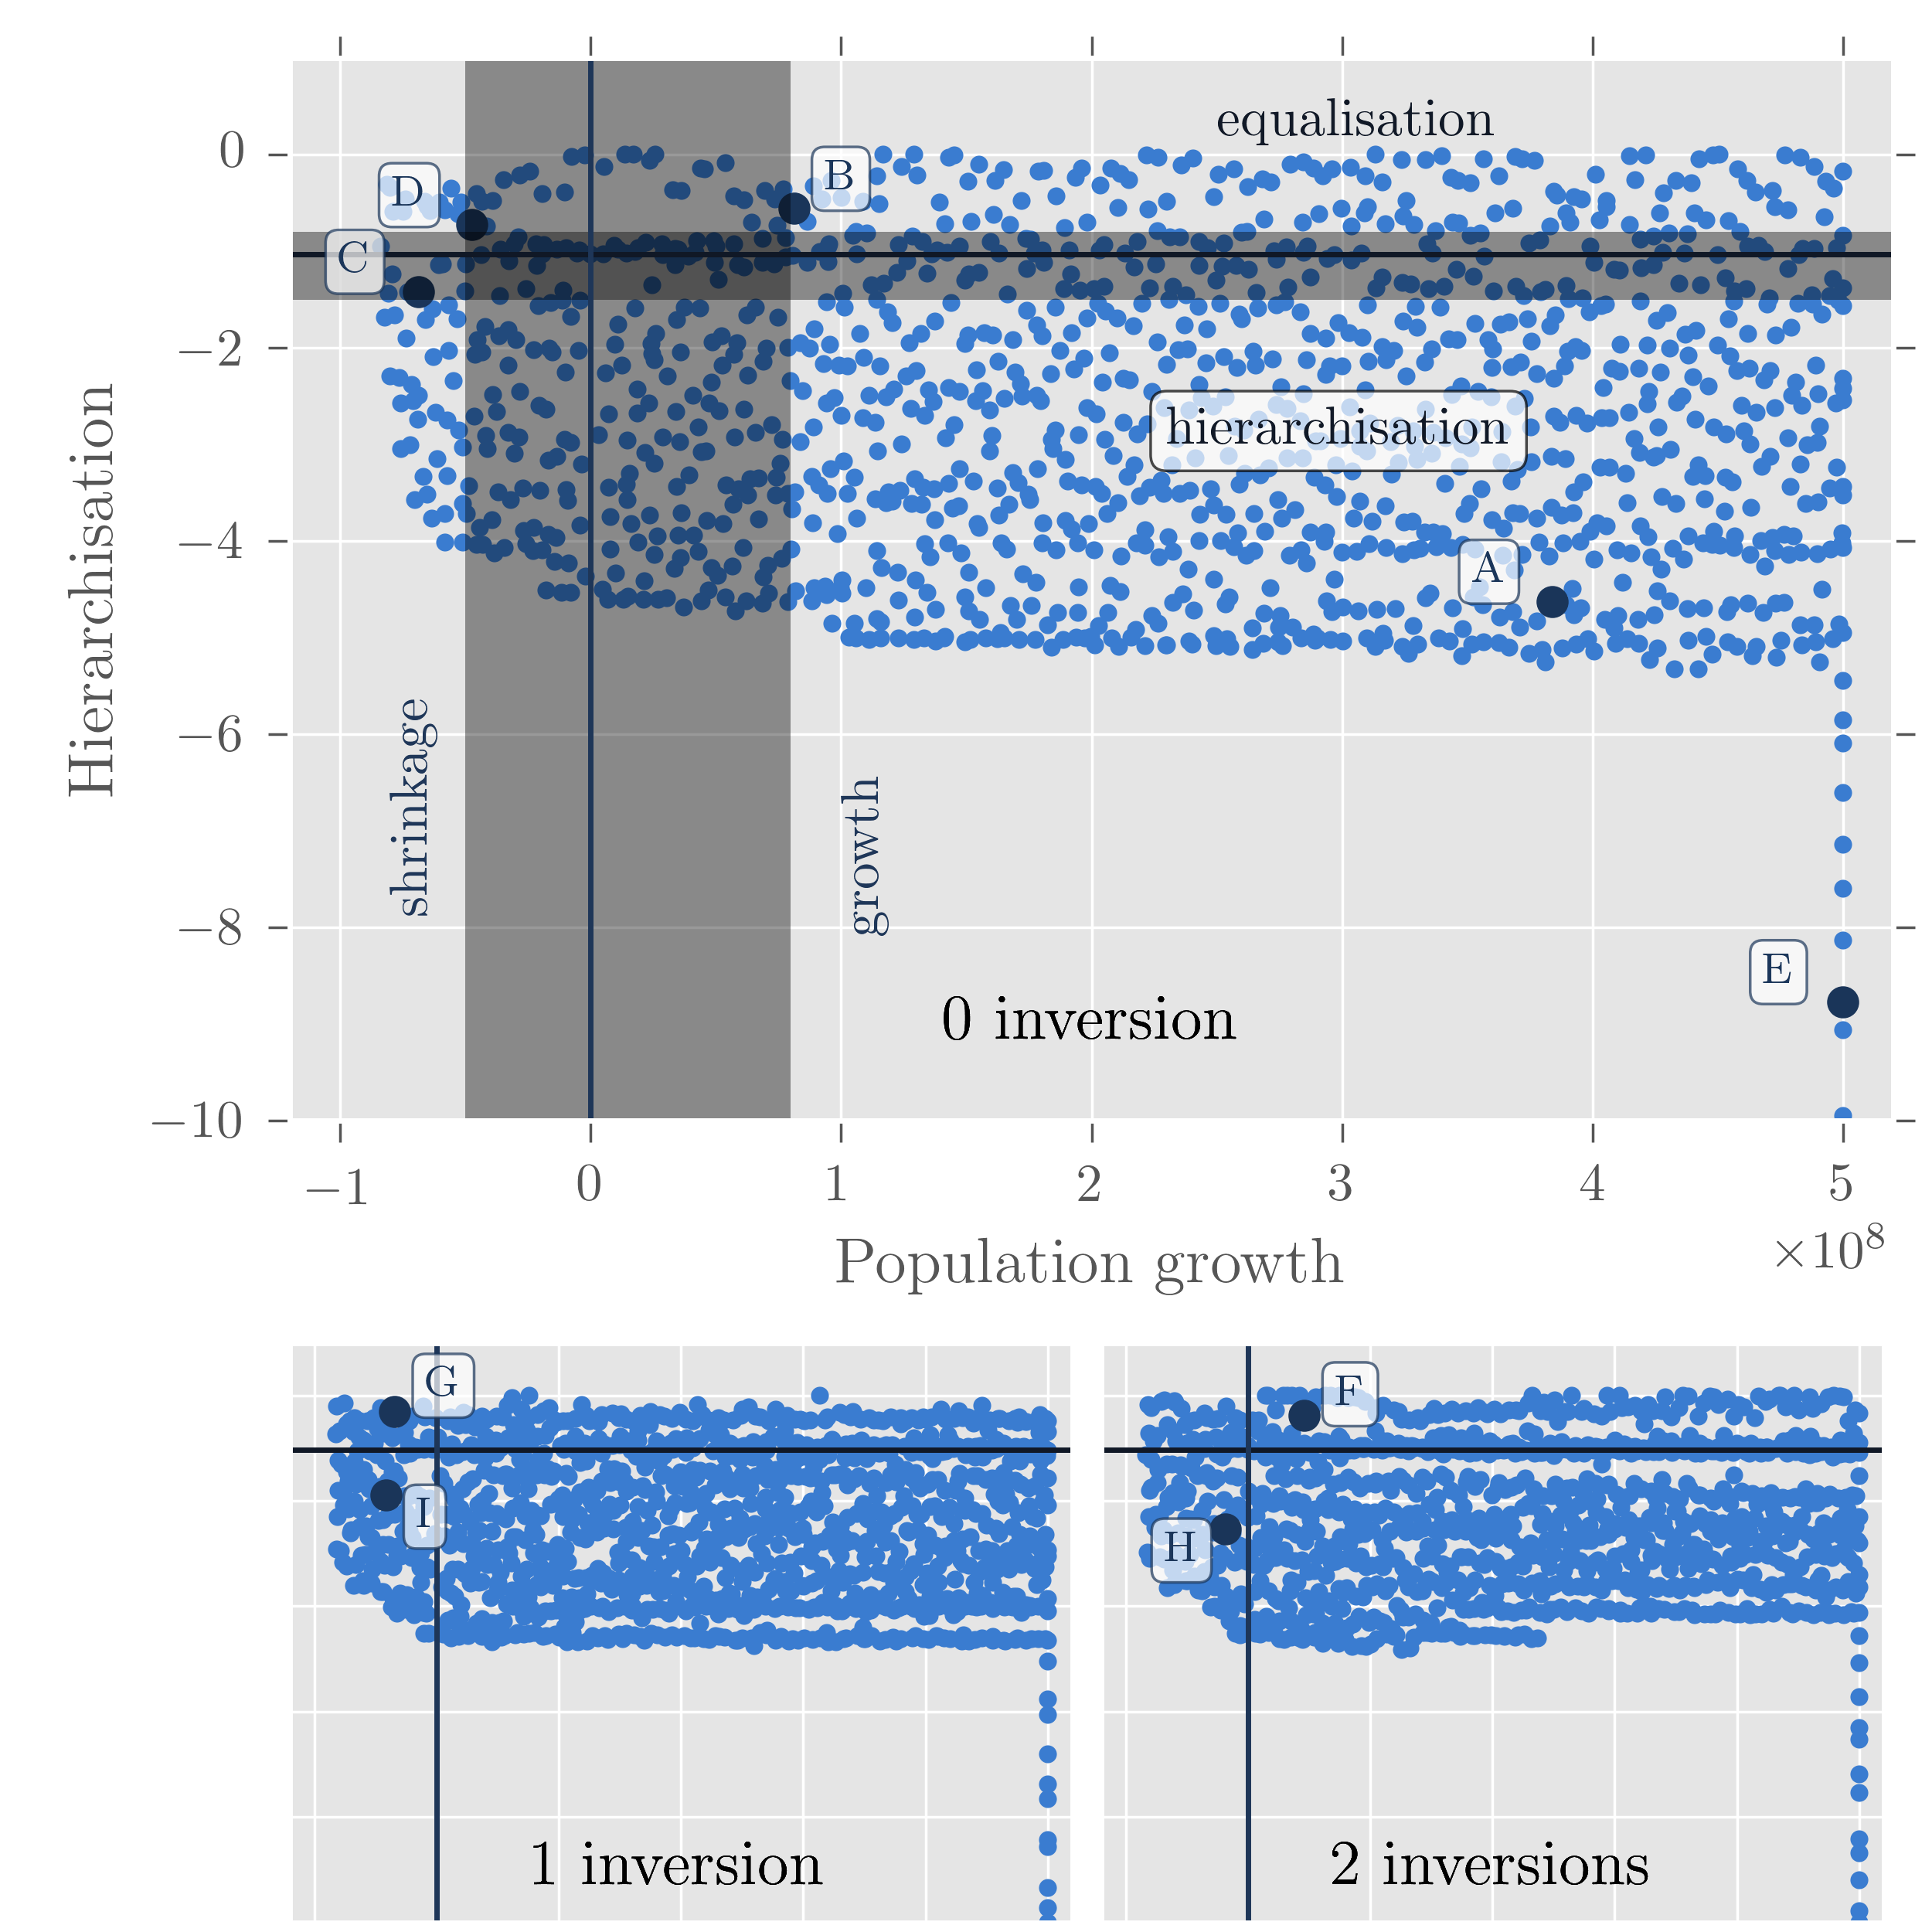
\includegraphics[width=0.6\textwidth]{figures/pse_marius.png}

%Interpretation
%All expected/observed patterns are produced: the model is generic enough.
%
%
%Unexepected patterns are found:
%
%aberations: better constrain the model,
%predictions: test them.

% Exemple OpenMOLE + SimPLU (IGN) https://simplu.openmole.org/

}

\sframe{Problème inverse}{


\centering

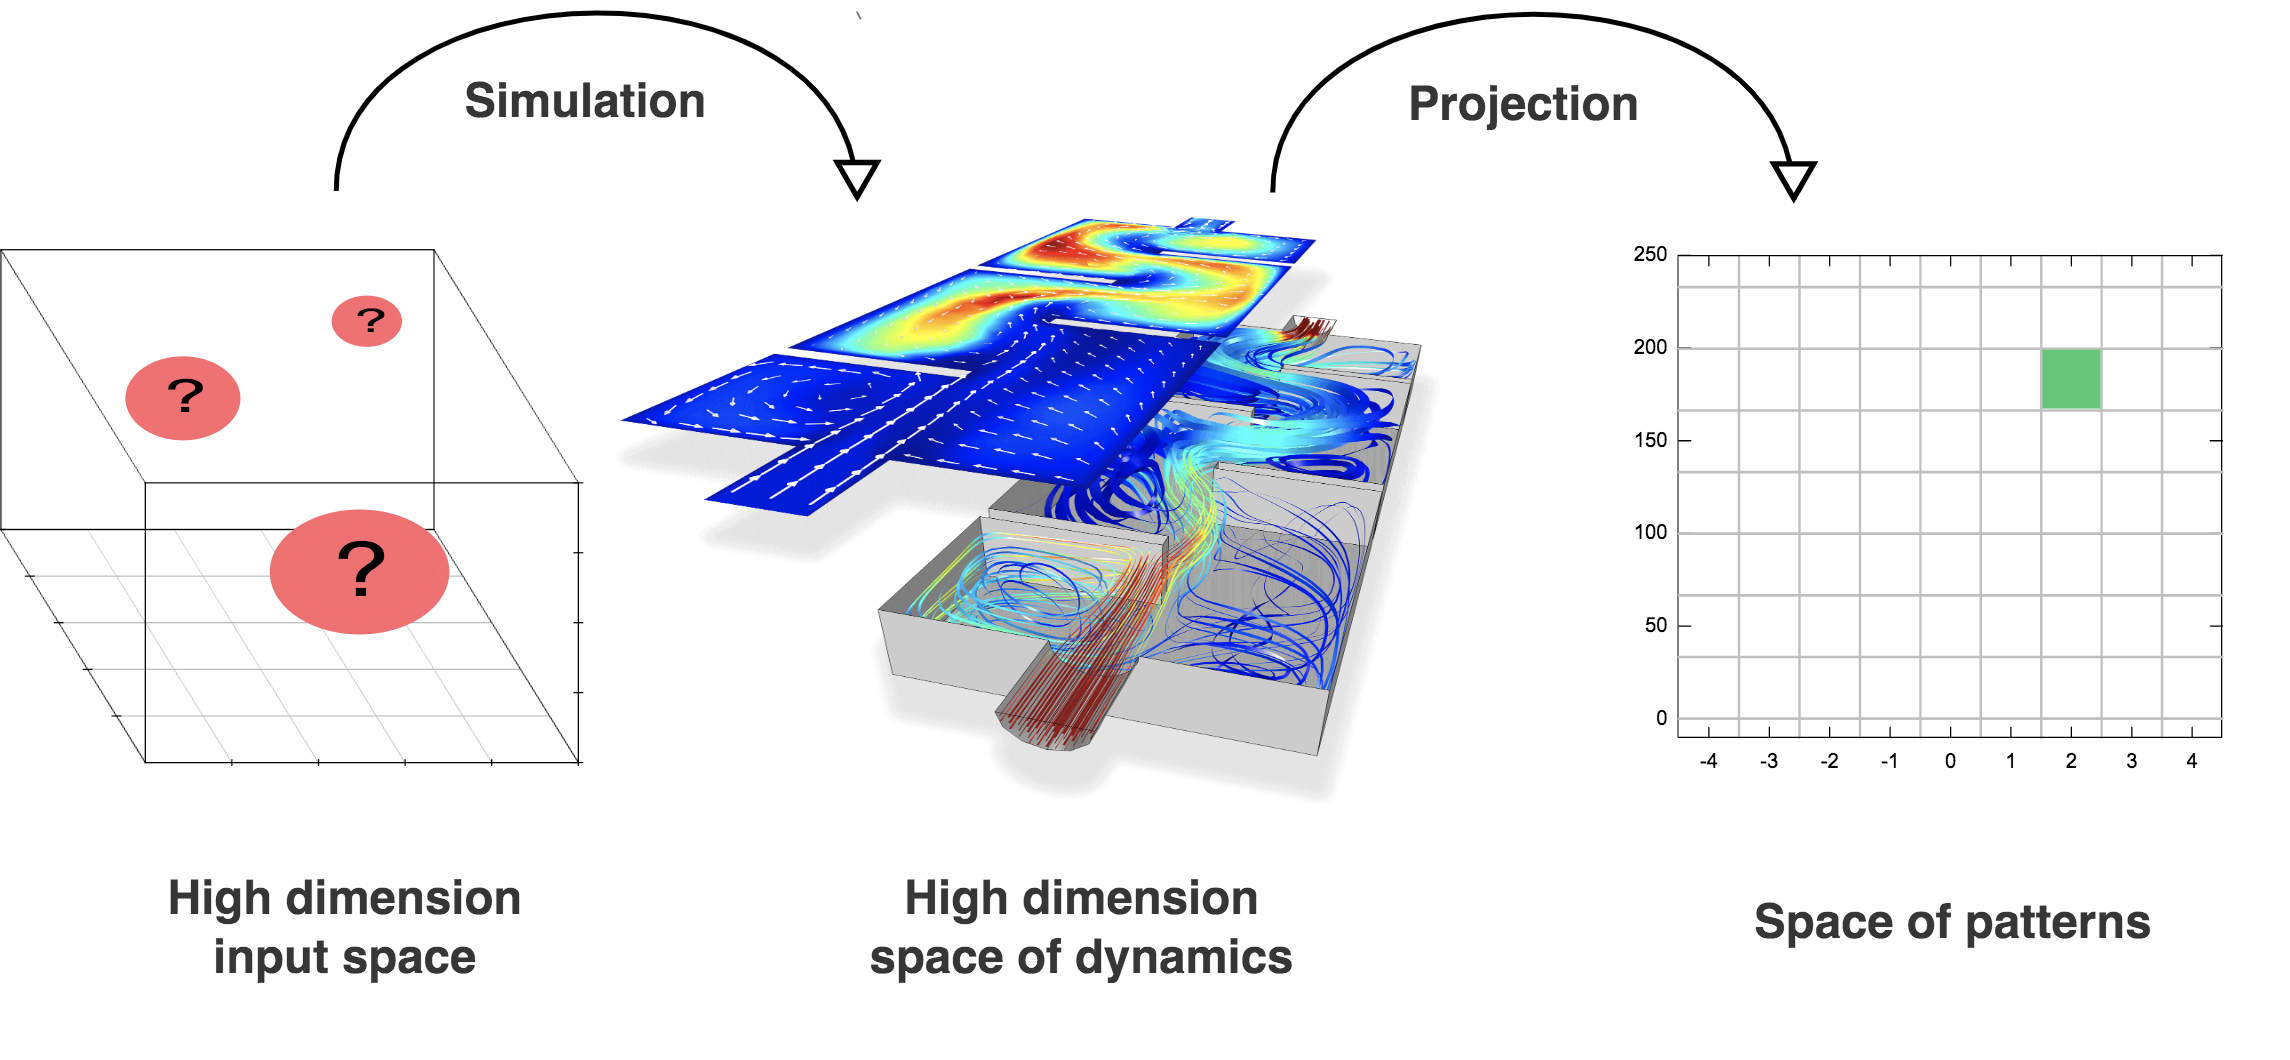
\includegraphics[width=\textwidth]{figures/ose_algo.png}

}


\sframe{Résultats : minimisation d'une fonction de Rastrigin}{

Formulation: $\Delta$ pattern < $\varepsilon$ %($f(x_1,\ldots, x_n) < 10$)

\centering

%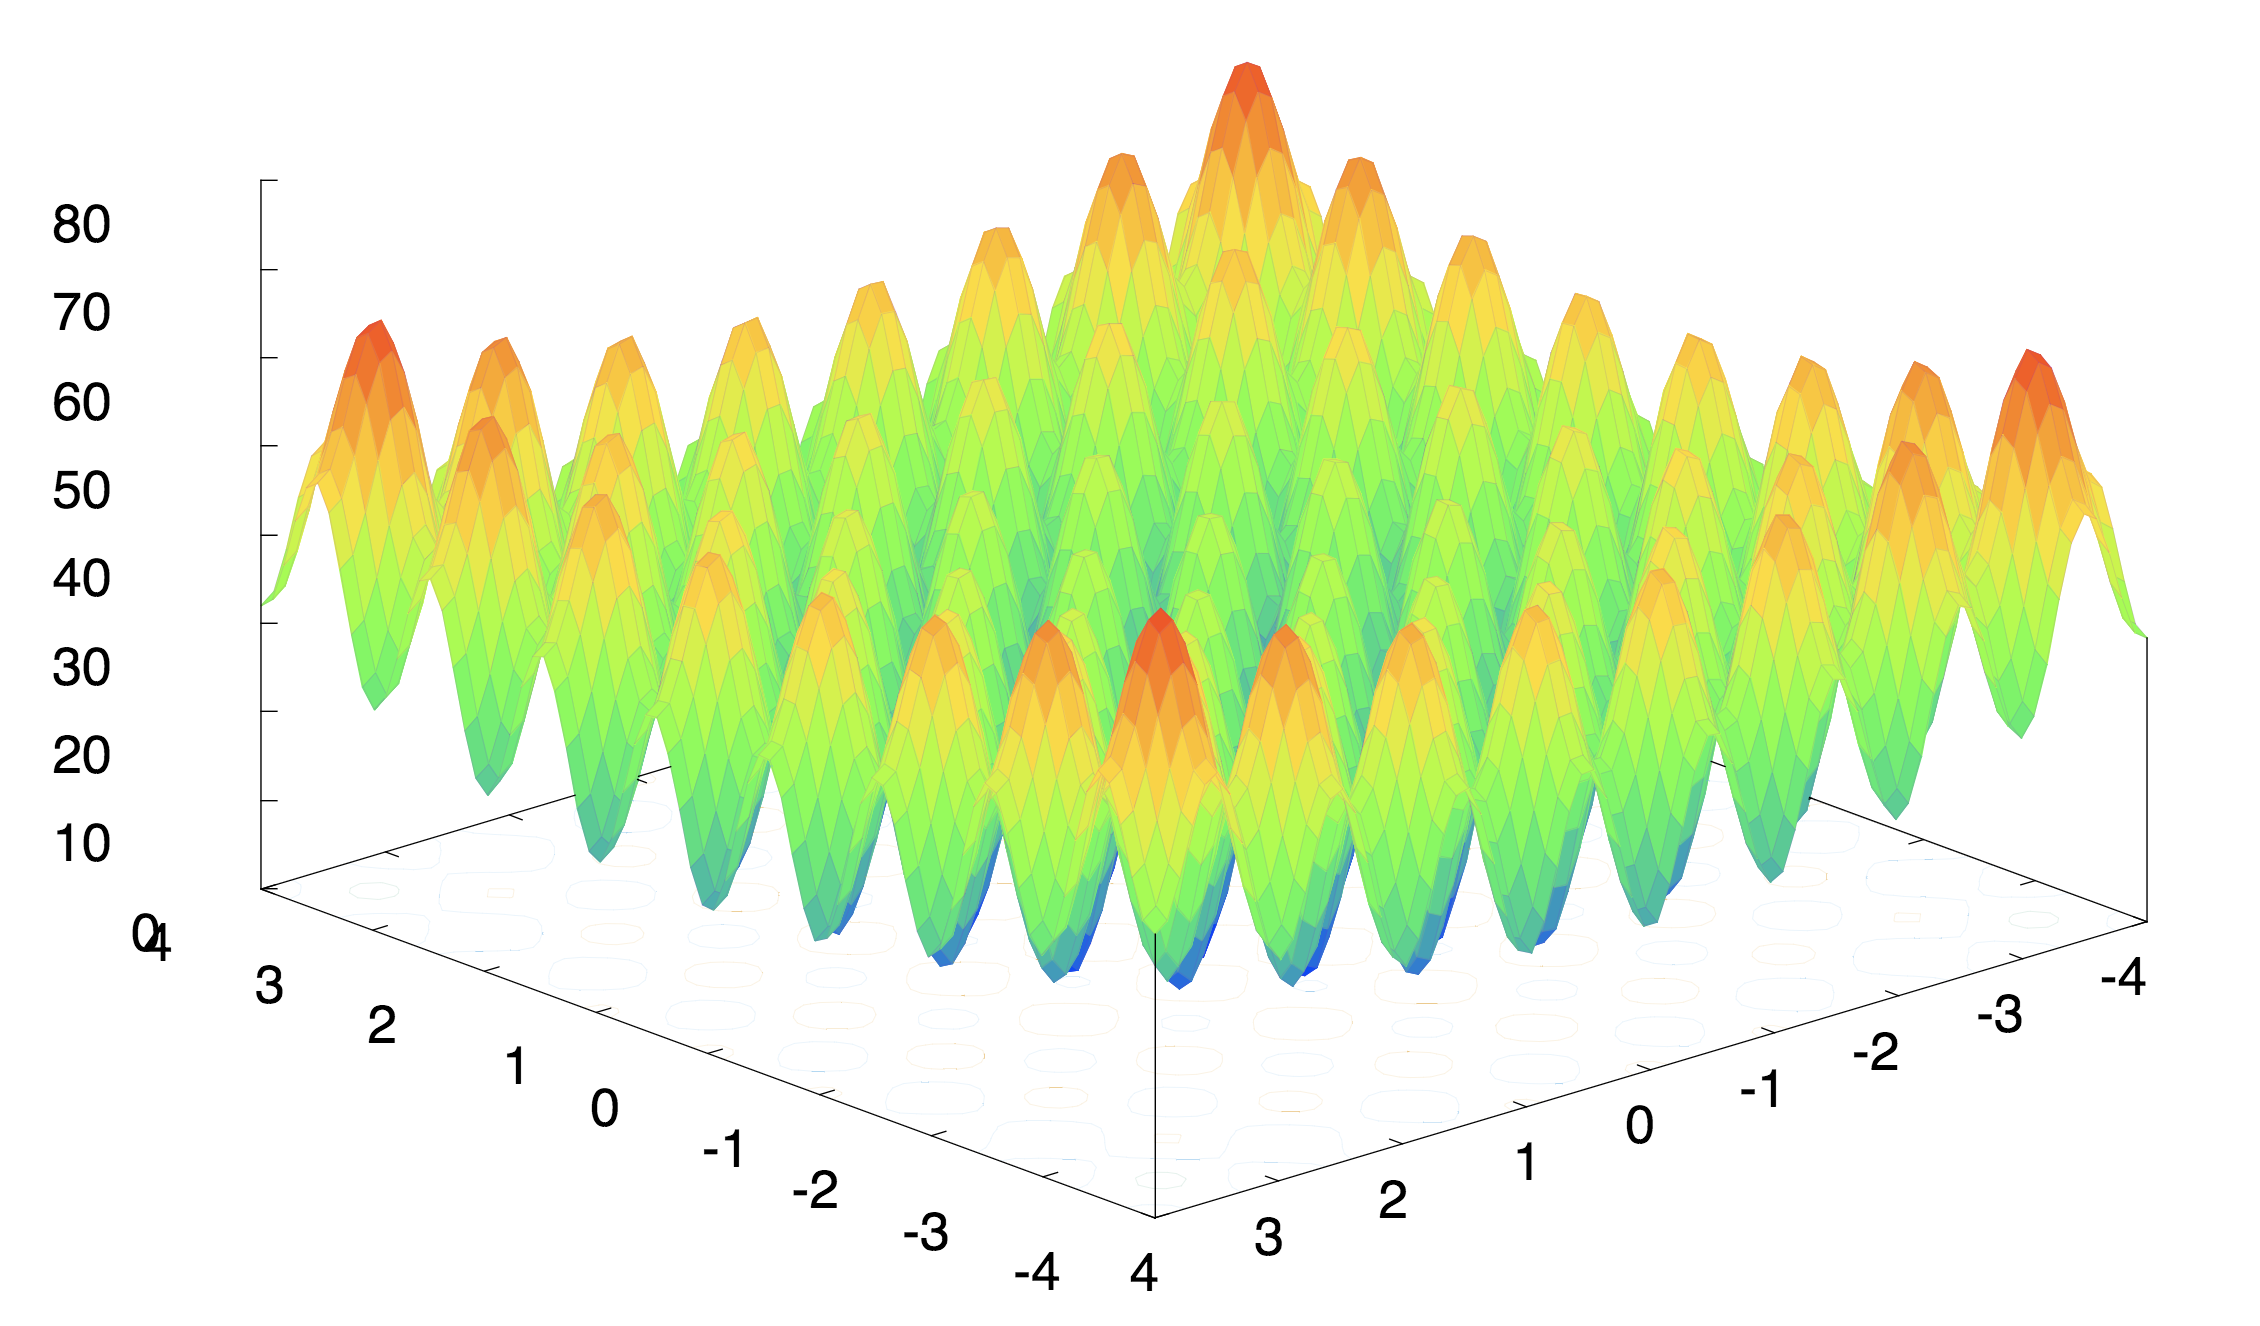
\includegraphics[width=\textwidth]{figures/rastrigin.png}
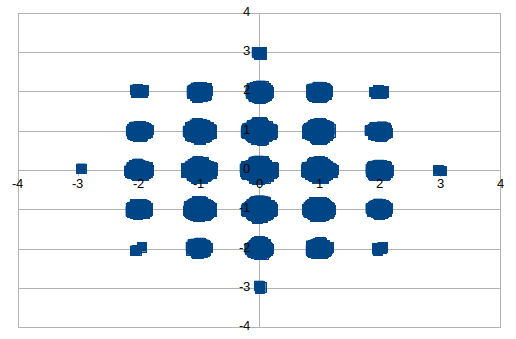
\includegraphics[width=\textwidth]{figures/oserast6d.png}

%6-D Rastrigin function < 10

}



\sframe{Analyse de sensibilité spatiale}{



\centering

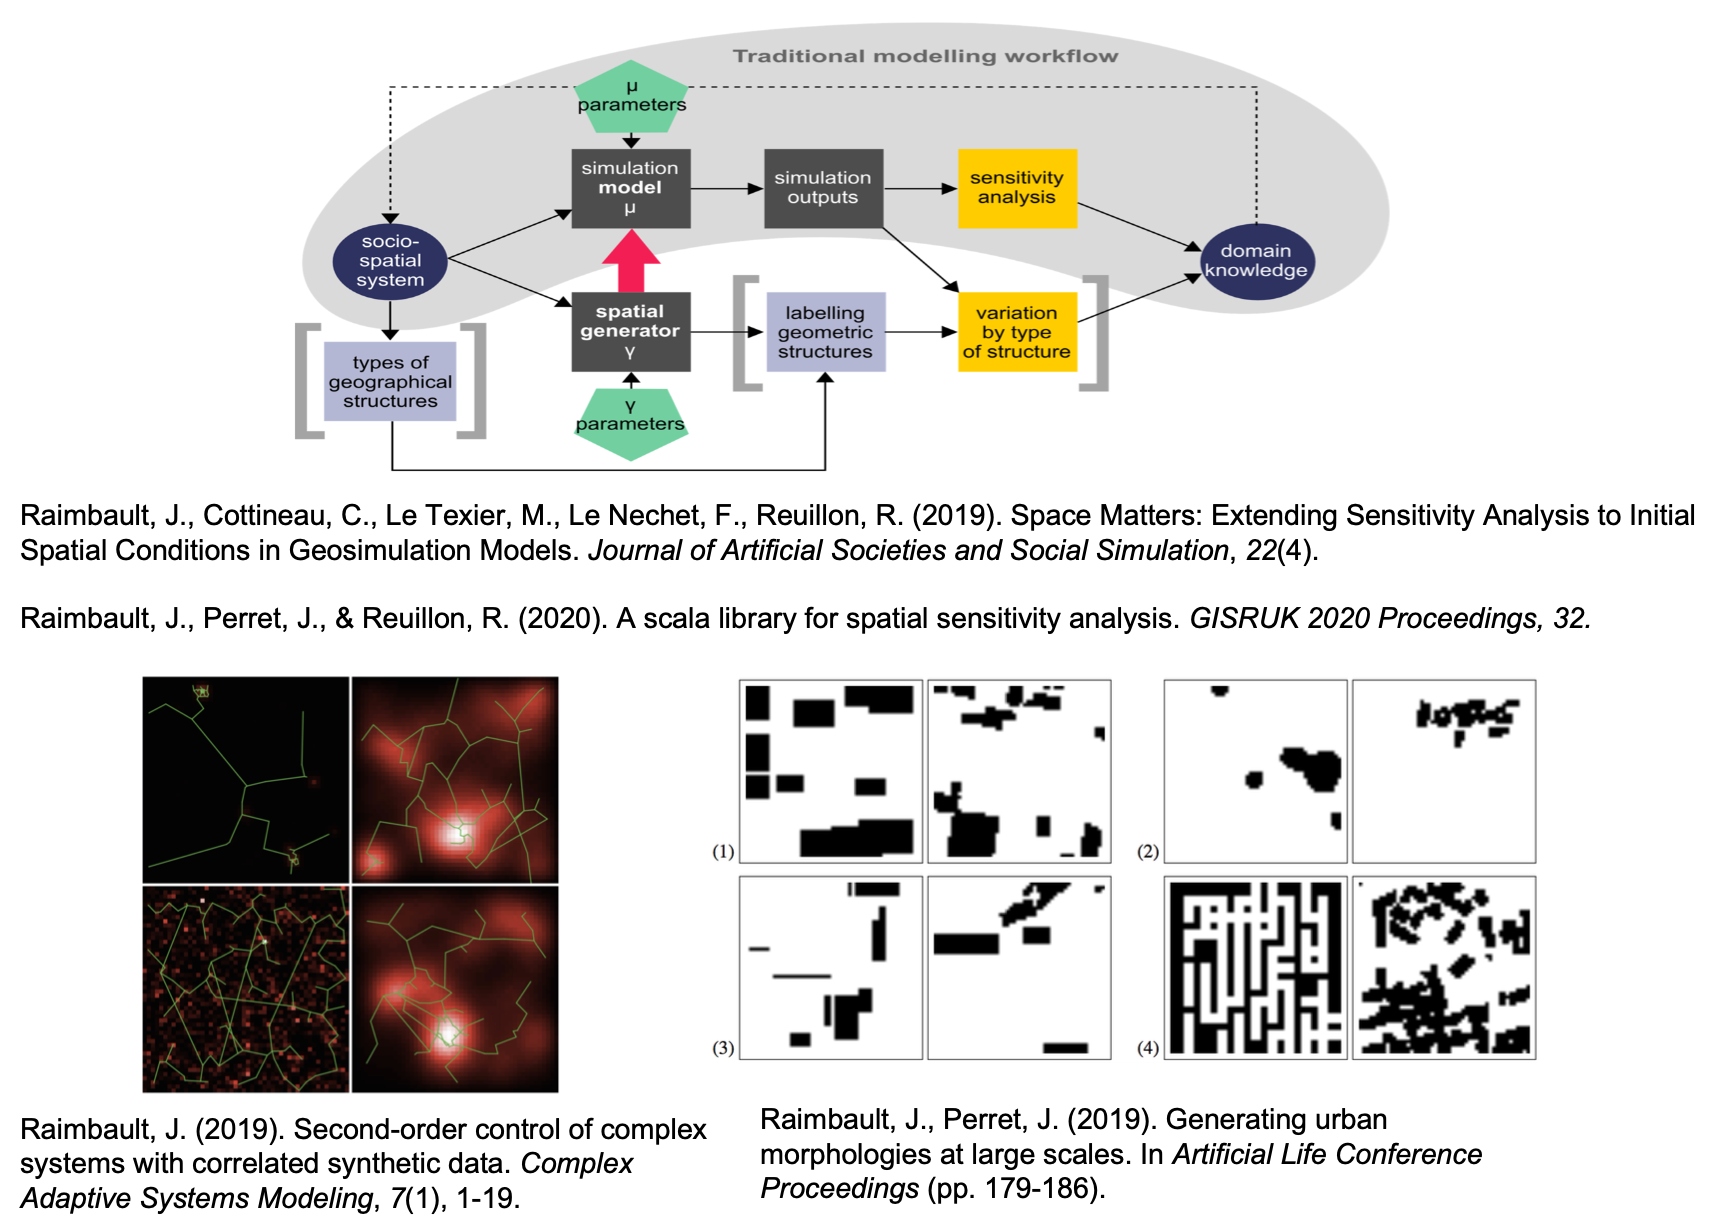
\includegraphics[width=0.95\linewidth]{figures/spatial_sa.png}

\nocite{raimbault2019second}
\nocite{raimbault2019generating}
\nocite{raimbault2019space}

}




\sframe{Couplage de modèles}{

\justify

\textit{Modèle de transport à quatre étapes modulaire en utilisant des briques et données ouvertes}

\bigskip

\textbf{Modèles intégrés :}

\begin{itemize}
	\item MATSim (MATSim Community) pour le transport \cite{w2016multi}
	\item SPENSER (University of Leeds) pour la population synthétique \cite{spooner2021dynamic}
	\item QUANT (CASA, University College London) pour les interactions spatiales \cite{batty2021new}
	\item spatialdata library (OpenMOLE community) pour les données spatiales \cite{raimbault2020scala}
\end{itemize}

\smallskip

\tiny

Raimbault, J., \& Batty, M. (2021). Estimating public transport congestion in UK urban areas with open transport models. GISRUK 2021 Proceedings.

\nocite{raimbault2021estimating}

}


\sframe{Couplage de modèle : urbanisme et îlot de chaleur}{

\begin{columns}
	\begin{column}{0.6\linewidth}
		\begin{center}
			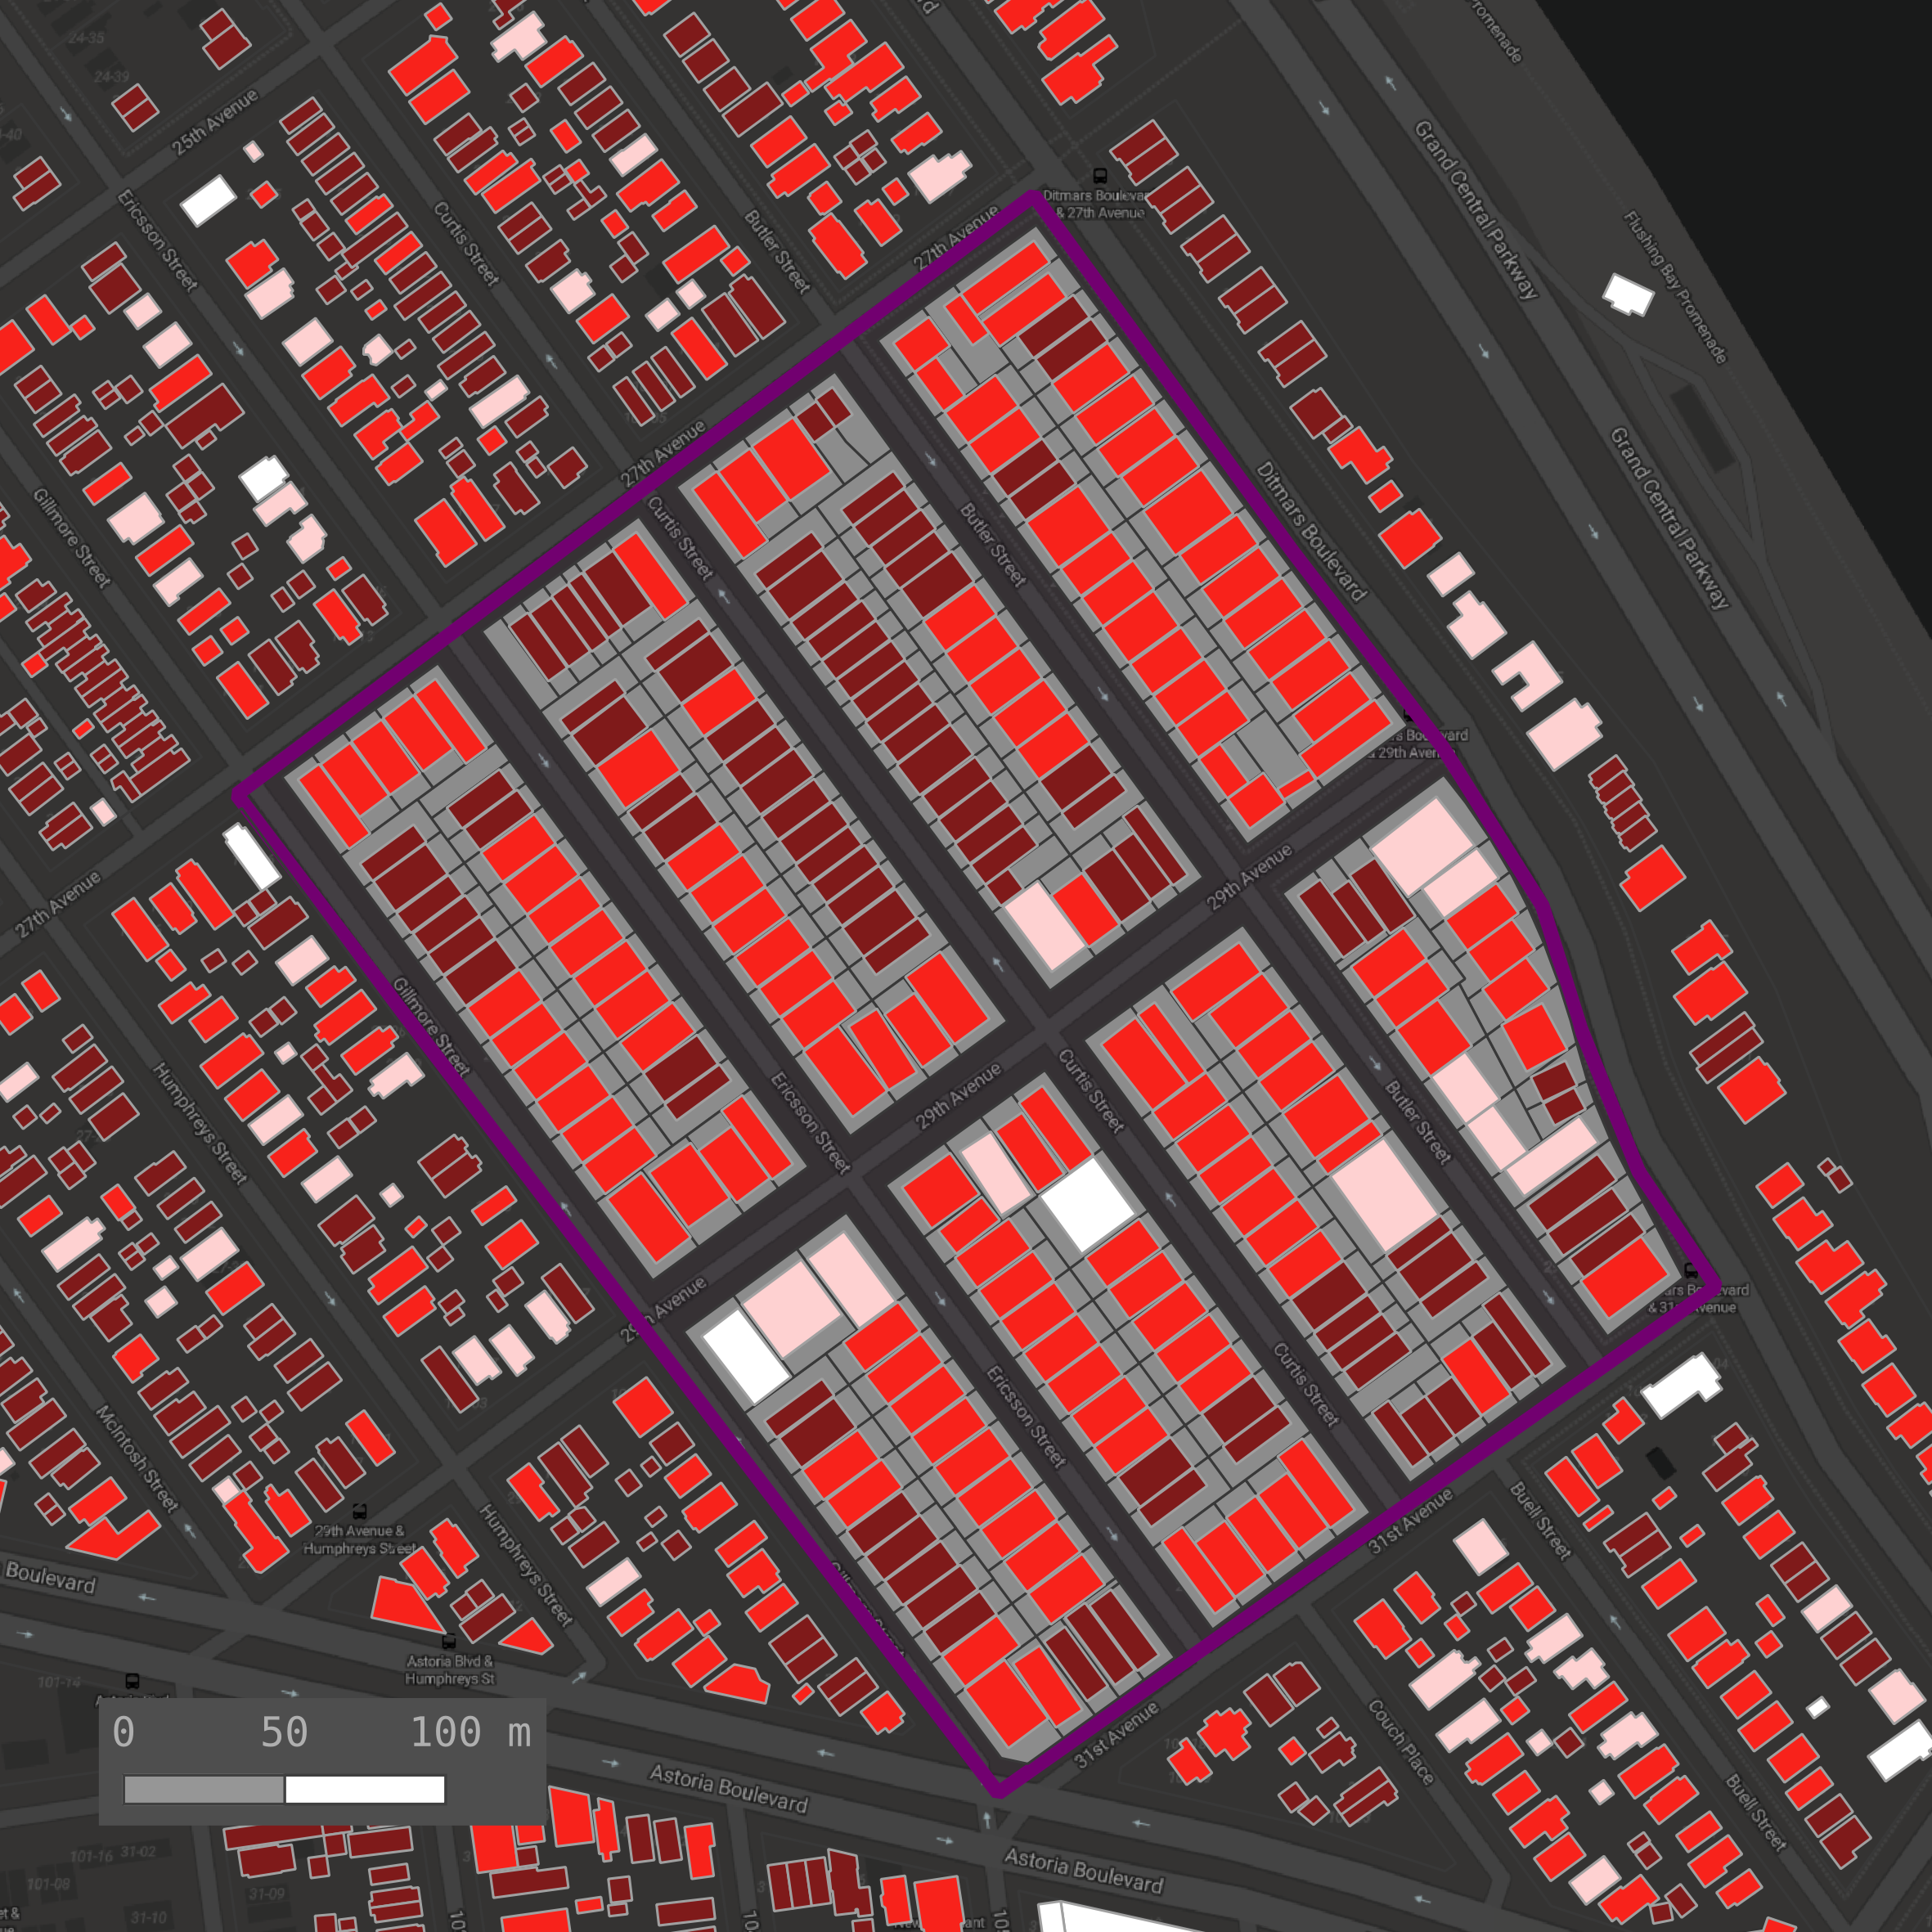
\includegraphics[width=\linewidth]{figures/buildings_6.png}	
		\end{center}
	\end{column}
	\begin{column}{0.39\linewidth}
		\justify
		\textbf{Projet SURe} (collaboration LASTIG, ISC-PIF, EPIDAPO)
		
		\bigskip
		
		$\rightarrow$ couplage du modèle SimPLU3D \cite{brasebin2017apports} avec un modèle d'îlot de chaleur urbain pour trouver des compromis entre densité et UHI.

	\end{column}
\end{columns}




}



\sframe{Couplage de modèles : vers des modèles multi-échelles}{



\begin{center}
	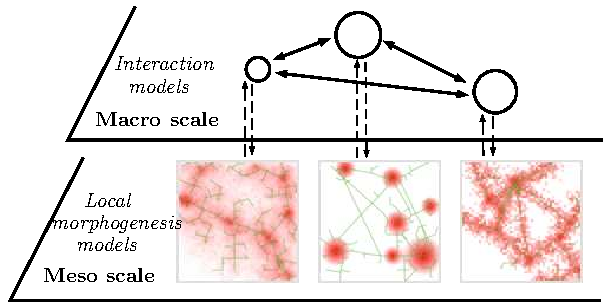
\includegraphics[width=0.75\textwidth]{figures/multiscale_morph.pdf}
\end{center}

\medskip

\textit{Processus spécifiques aux échelles, le couplage nécessite des ontologies dédiées} 

\medskip

\tiny

Raimbault, J. (2021). Strong coupling between scales in a multi-scalar model of urban dynamics. arXiv preprint arXiv:2101.12725.

\nocite{raimbault2021strong}

\smallskip

Raimbault, J. (2021). A multiscale model of urban morphogenesis. arXiv preprint arXiv:2103.17241.

\nocite{raimbault2021multiscale}

\smallskip

Raimbault, J. and Pumain, D. (2023). Innovation dynamics in multi-scalar systems of cities. \textit{ALIFE 2023}.


}



\sframe{Synthèse : benchmark d'OpenMOLE}{

\centering

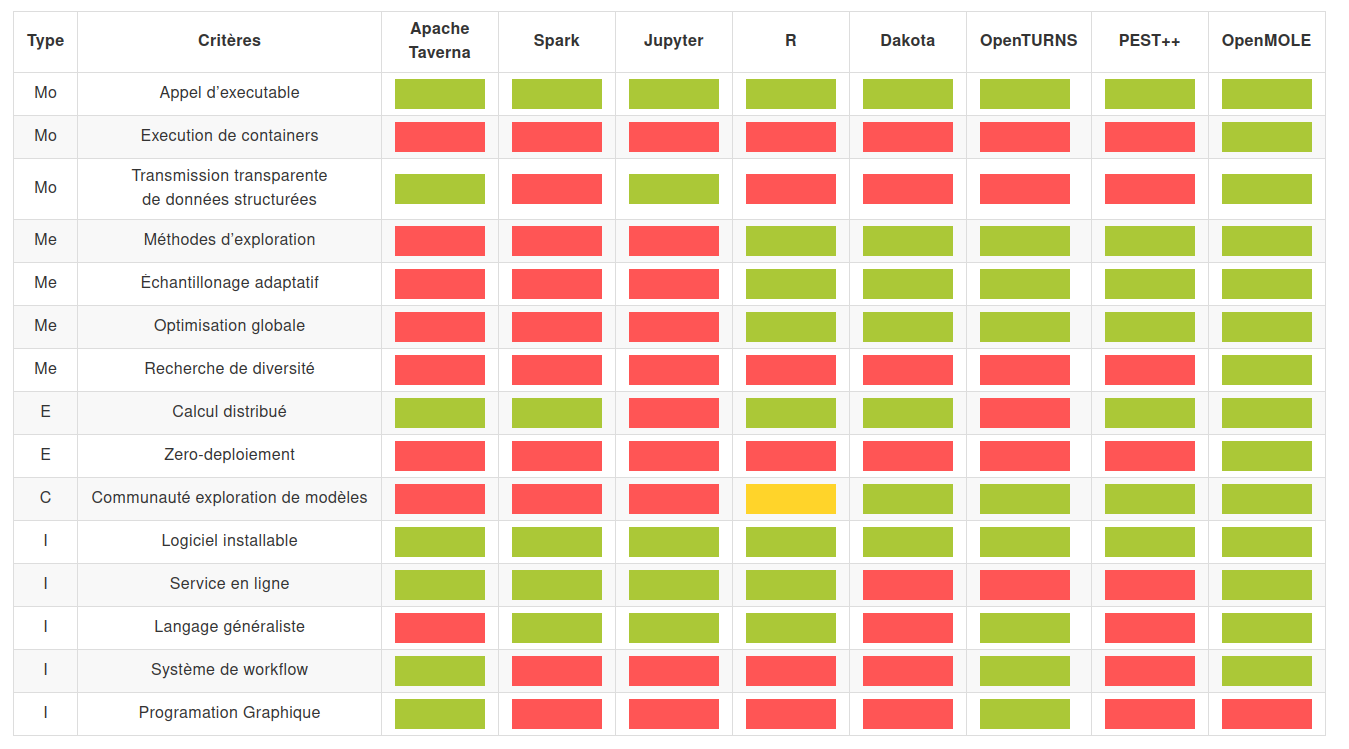
\includegraphics[width=\textwidth]{figures/openmole_benchmark.png}

}



\sframe{Utiliser OpenMOLE}{

% use -> download, compile, doc ; openmole.org github.com/openmole/openmole

\begin{center}
	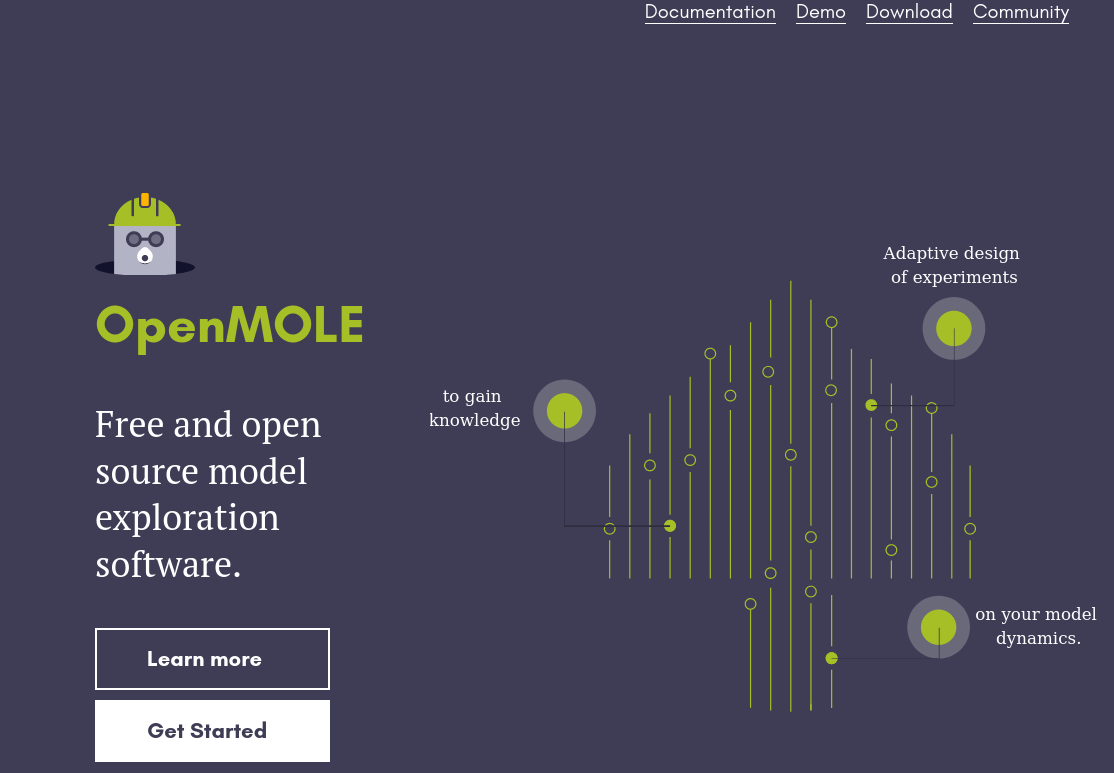
\includegraphics[width=0.7\textwidth]{figures/website.png}
\end{center}

\smallskip

\footnotesize

$\rightarrow$ Executable java sans installation sur \texttt{https://openmole.org}, code source à compiler sur \texttt{https://github.com/openmole/openmole}

$\rightarrow$ Demande d'une instance en ligne personnelle sur \texttt{https://my.openmole.org} : contacter l'équipe de développement

}

\sframe{Aide et contribution}{

% use / contribute : chat- - active community - coding camp

\begin{center}
	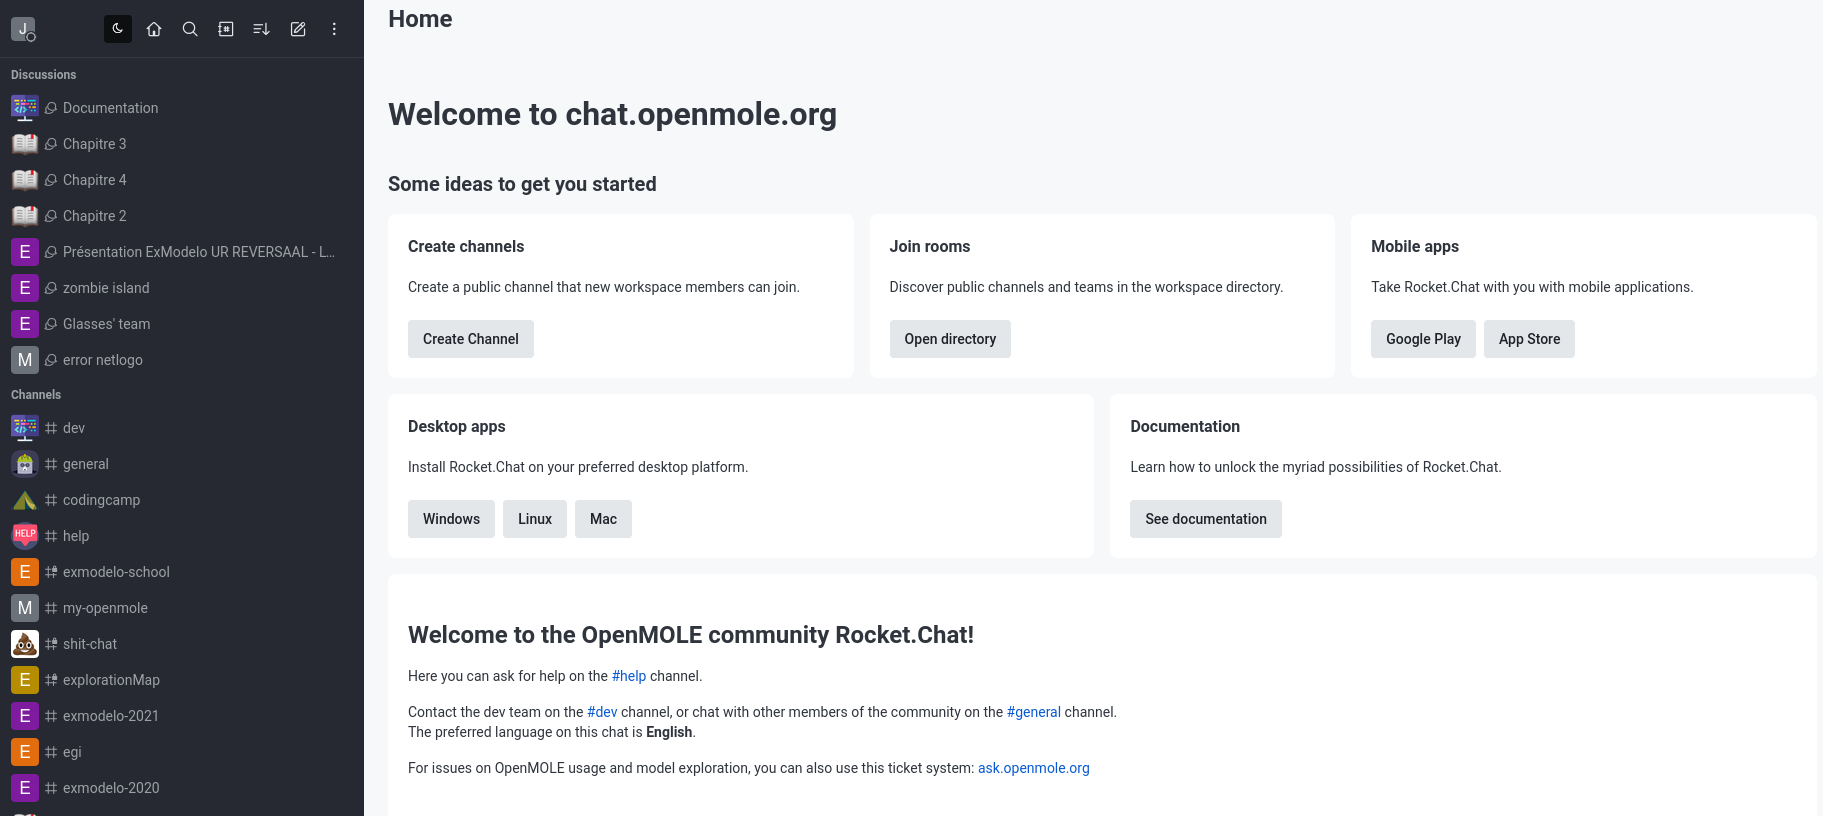
\includegraphics[width=\textwidth]{figures/chat.png}
\end{center}

\smallskip

Chat très réactif : \texttt{https://chat.openmole.org}

\medskip

Coding camp annuels début juillet : n'hésitez pas à nous contacter pour participer en 2024 !

\medskip

Communauté à l'IGN (LASTIG, Strudel) : Paul Chapron, Julien Perret, Juste Raimbault

}

\sframe{Contribution}{


\begin{center}
	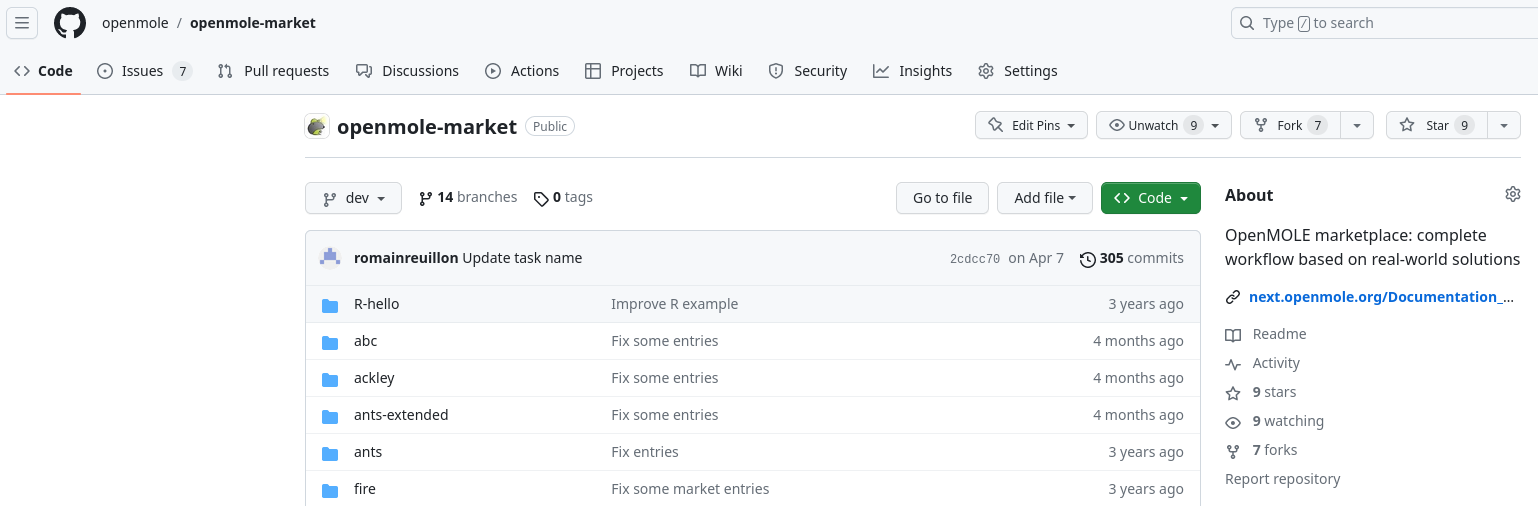
\includegraphics[width=0.9\textwidth]{figures/market_gh.png}\\\bigskip
	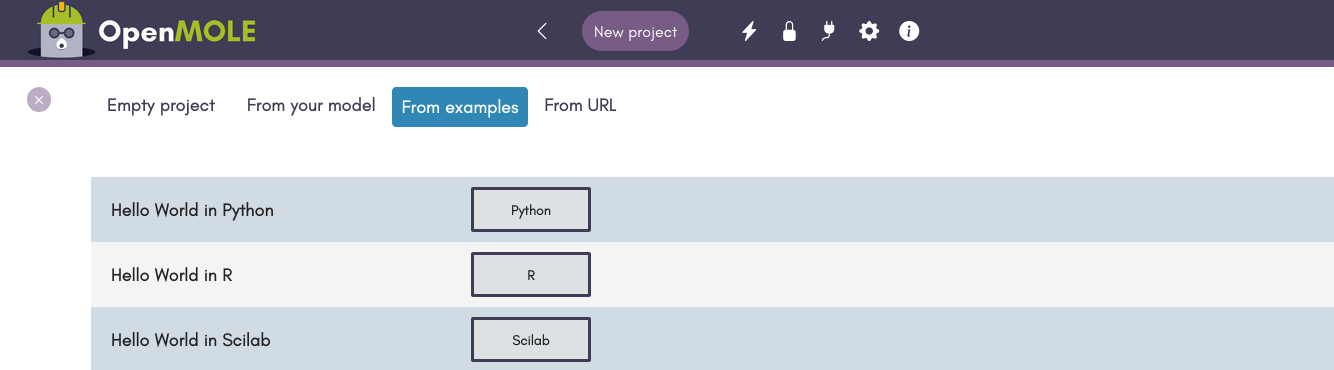
\includegraphics[width=0.9\textwidth]{figures/market_gui.png}
\end{center}

\bigskip

Ajouter des exemples thématiques et accessibles divers au market \texttt{https://github.com/openmole/openmole-market}

}

\sframe{Formation}{

% learn: exmodelo


\begin{center}
	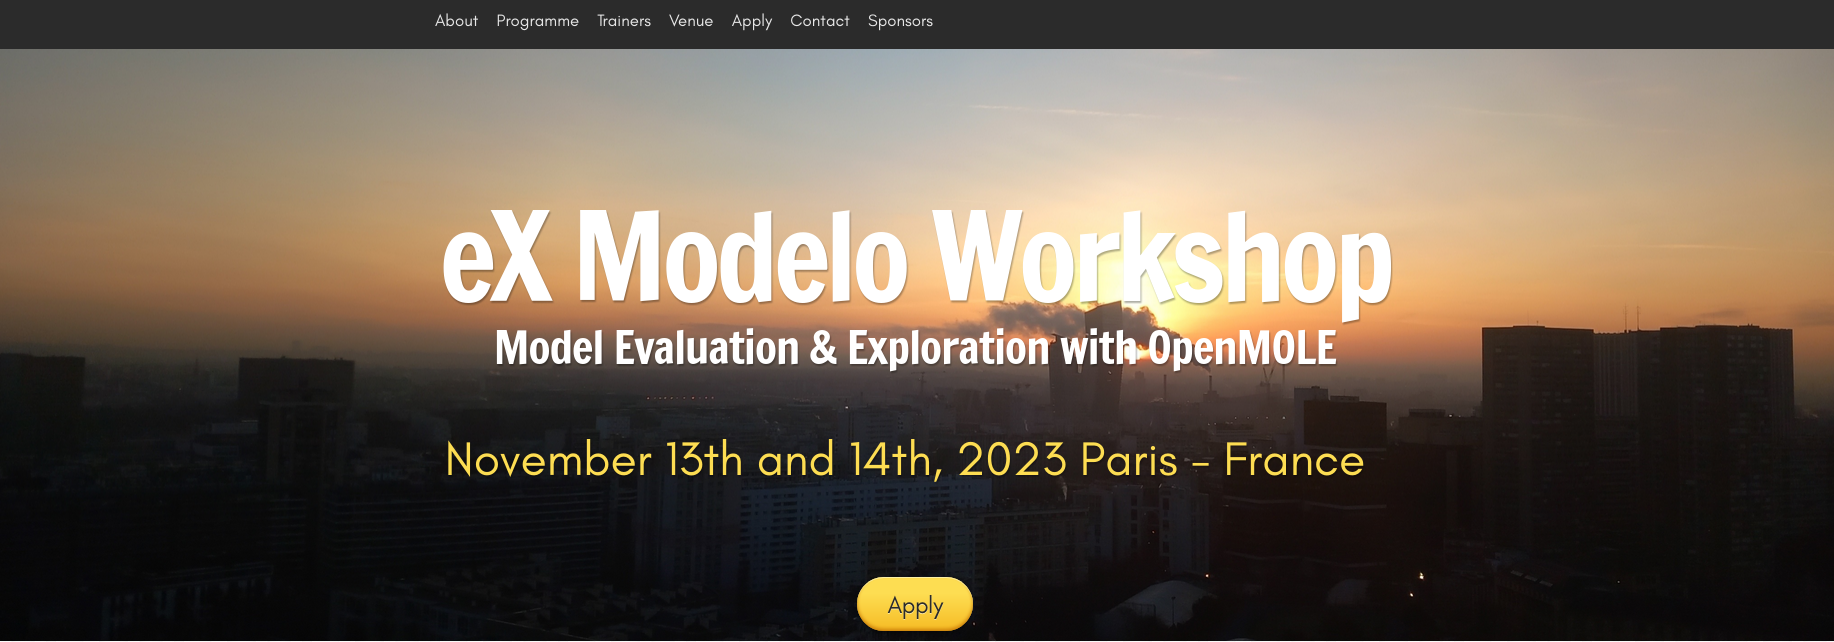
\includegraphics[width=\textwidth]{figures/exmodelo.png}
\end{center}

\medskip

Journées de formation ExModelo (ISC-PIF, novembre) \texttt{https://workshop.exmodelo.org/} : candidatures ouvertes (participation gratuite), dans l'héritage des 3 éditions de l'école d'été



}

\sframe{Conseil scientifique et R{\&}D}{

\begin{center}
	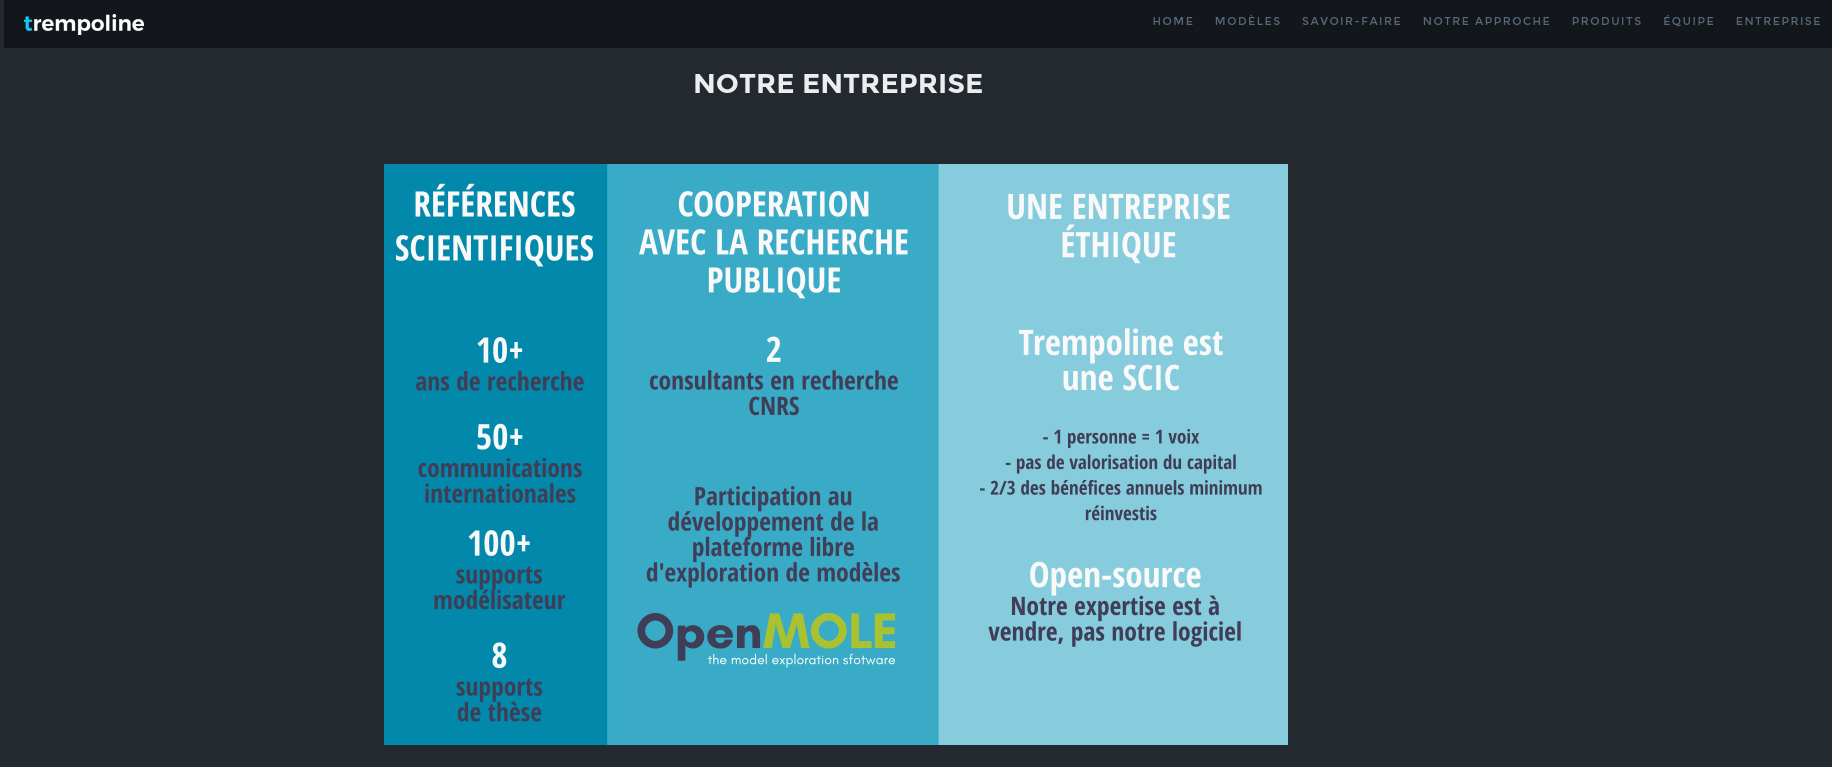
\includegraphics[width=\textwidth]{figures/trempoline.png}
\end{center}




}



\sframe{Résumé du positionnement d'OpenMOLE}{

%\textit{A qualitative shift in knowledge that can be extracted from a simulation model with model exploration methods.}

\textit{Un saut qualitatif dans la connaissance extraite d'un modèle de simulation par les méthodes d'exploration des modèles}

\medskip

%Success stories: SimpopLocal \cite{schmitt2014half}, Marius \cite{10.1371/journal.pone.0138212}, Ecological modeling \cite{lavallee2018dynamical}, epidemiology \cite{arduin2018modelisation}, etc.

Exemples pluridisciplinaires : SimpopLocal \cite{schmitt2014half}, Marius \cite{10.1371/journal.pone.0138212}, modélisation en écologie \cite{lavallee2018dynamical}, en épidémiologie \cite{arduin2018modelisation}, etc.

\medskip

\textbf{Caractéristiques principales : }

$\rightarrow$ Role unique des axes complémentaires de l'accès aux environnements, de la disponibilité des méthodes, et de l'embarquement des modèles.

$\rightarrow$ Construction itérative et intégrée des modèles et théories, en utilisant l'ensemble des dimensions de la connaissance favorisées par la simulation et le calcul (modélisation, théorie, empirique, données, méthodes, outils \cite{raimbault2017applied}).

$\rightarrow$ Couplage des modèles et reproductibilité au coeur de l'approche par workflow \cite{passerat2017reproducible}.


% brique du jumeau?

\bigskip

\large \textbf{!! Une brique essentielle pour la partie simulation du futur Jumeau Numérique !!}



}







%%%%%%%%%%%%%%%%%%%%%
\begin{frame}[allowframebreaks]
\frametitle{References}
\bibliographystyle{apalike}
\bibliography{/home/JRaimbault/ComplexSystems/CityNetwork/Biblio/Bibtex/CityNetwork,biblio}
\end{frame}
%%%%%%%%%%%%%%%%%%%%%%%%%%%%




\end{document}









